
\chapter{Electrochemical stability of metal and oxide catalysts in the presence of nitrogen ligands}

\section{Introduction}
With a rapidly growing global population, the demand for ammonia-based fertilizers continues to increase, placing additional strain on the nitrogen cycle. Traditionally, nitrogen-based fertilizers are produced from ammonia synthesized through the Haber-Bosch process, which remains vital for the sustainability of agricultural productivity \cite{Schloegl2003CatalyticStory}. However, the Haber–Bosch reaction operates at high temperatures (250 to 400~$^\circ$C) and pressures (100 to 300~bar) \cite{Smil1999DetonatorExplosion,Erisman2008HowWorld, Lim2021Ammonia2050,Verleysen2021HowStorage}, relies on fossil-derived hydrogen, and leaves a significant carbon footprint \cite{Liu2022ProspectsFixation, Smil1999DetonatorExplosion,Suryanto2021NitrogenShuttle}. In contrast, organic waste from sewage and farms offers an alternative resource for reduced nitrogen\cite{ChipocoHaro2024ElectrocatalystsConversion,Adebayo2004EvaluationFingerlings,Mulchandani2016RecoverySludges}, which constitutes 15\% of total nutrients in the sludge\cite{Xiao2020ProteinReview, Thomsen2017ChangesSludge}. The organic matter dissolved in sludge includes nucleic acids, humic acids, proteins and polysaccharides\cite{Jung2002RecoverabilityWastewater}. Electrochemical methods, such as the electrolysis of waste-activated sludge (EWAS), offer a more sustainable pathway to recover nitrogen while mitigating environmental impacts operating at low temperature\cite{Botte2024InnovativeRecovery,Vedharathinam2014ExperimentalMedium,Alvarez-Pugliese2024PerspectivesWaste, Zeng2019ElectrochemicalSulfide,Ye2016ElectrochemicalProduction}. 

Existing EWAS methods rely on high applied cell voltages, ranging from 5 to 30~V, to drive oxidation and nitrogen transformation in sludge. This results in the formation of reactive oxygen species, which often compete with nitrogen species for active sites on the electrode surfaces. Although Jafari et al.\cite{JafariElectrochemicalProduction} explored lower-voltage electrolysis to mitigate these side reactions, the resulting systems suffered from low current density (<30~mA~cm$^{-2}$) and low yield (<5$_{\rm mass}\%$)\cite{Zhao2022AAmmonia}. Therefore, the development of efficient, robust catalysts that can operate at mild voltages without sacrificing performance remains a key challenge for EWAS.

A major limitation of EWAS lies in the stability of the catalyst under nitrogen-rich and oxidative conditions. Elevated potentials accelerate electrode corrosion and dissolution\cite{Sanchis2022NitrateOverview,Popov2015ThermodynamicsCorrosion,Kapaka2010ElectrochemicalElectrode,Mucalo2004InSolutions,Aksu2001ElectrochemistrySolutions,OConnor2018ElectrochemicalSolutions}, while competition between nitrogen oxidation and OER further degrades catalytic performance~\cite{Li2021Ru-DopedNitrate,Wang2022ElectrochemicalOxidation,Dai2020ElectrochemicalOxides}. Reactive nitrogen species, such as ammonia (\ce{NH3}), glycine, and cyanide (\ce{HCN}), can form metal-ligand complexes that promote leaching and surface degradation~\cite{Bjerrum1957StabilitySubstances,Meng1996PrinciplesReview,Wang2022AmmoniaSystem}. While metal leaching in ammonia, cyanide, and glycine solutions has been extensively studied in hydrometallurgy~\cite{Meng1996PrinciplesReview,Wang2022AmmoniaSystem,Han1974AMMONIA-AMMONIUMNODULES,Bhuntumkomol1982TheSolutions,Azadi2021SustainableGlycine,Oraby2020GoldPermanganate,Sarvar2023ApplicationStructure,SPARROW1995CyanideApplications,Akcil2015PreciousReview}, these studies differ significantly from EWAS conditions, where ligand concentrations are lower and variable electrochemical driving forces influence material stability. Therefore, a systematic understanding of catalyst stability in nitrogen-rich environments under reducing and oxidative potentials in alkaline conditions is crucial for the development of efficient and sustainable electrodes.

Pourbaix diagrams provide a valuable framework for predicting electrode stability by mapping dissolution, passivation, and oxidation regimes as a function of pH and applied potential~\cite{PourbaixAtlasSolutions}. Traditionally used in corrosion studies~\cite{McCafferty2010ThermodynamicsDiagrams, Stack2005BridgingDiagrams,Pourbaix1973LecturesCorrosion}, Pourbaix diagrams help identify stable operating conditions where catalyst dissolution is minimized. Most of the available diagrams account primarily for interactions with hydrogen ions\cite{Huang2017ImprovedCompounds,Wang2020PredictingFunctional,Huang2015ElectrochemicalCalculations,Cao2020E-pHLaterite}, so extending them to nitrogen-containing ligands is necessary to provide insight into material stability under EWAS conditions. In hydrometallurgy, Pourbaix diagrams have been adapted to study metal leaching in nitrogen-containing solutions~\cite{Meng1996PrinciplesReview,NasuhaYahya2019ThermodynamicDiagram,Barragan2021LeachingOptimization,OConnor2018ElectrochemicalSolutions,Seke2006EffectSphalerite}. However, the direct application of these diagrams to electrocatalyst stability remains limited, due to the high concentration of nitrogen ligands, and the high temperatures and pressures used for metal leaching. Integrating Pourbaix stability analysis with computational and experimental validation can accelerate the identification of durable catalysts for EWAS.

Minimizing electrode dissolution is critical to ensuring both the sustainability of electrochemical oxidation and the safety of recovered fertilizers. In this study, we apply Pourbaix diagrams to EWAS, focusing on stability under nitrogen-rich conditions. By systematically analyzing potential-pH stability regions, we establish a computational framework for catalyst screening—highlighting stability as a key design criterion alongside activity and selectivity. This approach provides a pathway for developing robust and sustainable catalysts for electrochemical nitrogen recovery.


\section{Methods}
\subsection{Pourbaix Diagram Construction}
Pourbaix diagrams were constructed to map the thermodynamic stability regions of bulk metals/alloys and their metal-ligand complexes in the presence of nitrogen-containing ligands at concentrations in the range expected to be present in EWAS.
%under electrolysis of waste activated sludge (EWAS) potentials in basic environment. 
Free energies of bulk metals were obtained from the Materials Project database \cite{Jain2013TheInnovation}, based on generalized gradient approximation (GGA) density functional theory (DFT) calculations. Free energies for aqueous ligands and metal-ligand complexes were calculated from equilibrium constants sourced from standard thermochemical handbooks \cite{Wagman1982TheUnits, Smith1989CriticalConstants, Bard2017StandardSolution, Bjerrum1957StabilitySubstances} and literature \cite{Meng1996PrinciplesReview, Azadi2019DataComplexes, Aviles2022ExploringNH3, Oraby2023SelectiveSolutions, Harrington2005DeterminationIon}. We focus here on metal elements that are commonly used as electrode materials and those where metal-ligand complex stabilities are available: Au, Cu, Ni, Co, Mg, Mn, Ti, Zn, Ag, Cd, Sr, Pt, Pd and Fe. The aqueous ligands considered in this study include \ce{NH3-}, glycine and \ce{CN-}. The targeted experimental potential ranges from -2.0-2.3 V (vs RHE) and the pH ranges from 11.5-13.5, but Pourbaix diagrams are constructed over a wider range for reference.

\begin{equation} \label{eq:reaction}
aA + h\text{H}^+ + z\text{e}^- \leftrightarrow bB + \text{H}_2\text{O}
\end{equation}

The diagrams were constructed based the framework introduced by previous studies \cite{PourbaixAtlasSolutions, Huang2017ImprovedCompounds,Huang2015ElectrochemicalCalculations,Singh2017ElectrochemicalMaterials,Patel2019EfficientCompounds,Persson2012PredictionStates}. All reaction species, i.e. metals, alloys, oxides, aqueous ions and ligands, and water are connected by corresponding reactions. Then the reaction chemical potentials are derived from equilibrium relationships between species, using the Nernst equations, as a function of applied potential and pH. For a redox reaction shown in Equation~\eqref{eq:reaction}, the Nernst equation is:

\begin{equation} \label{eq:nernst} E = E^\circ - \frac{k}{z} \log \left(\frac{A^a}{B^b}\right) - \frac{k \cdot h}{z} \text{pH}, \end{equation}

where \(E\) is the cell potential at non-standard conditions, \(E^\circ\) is the standard electrode potential, and $k$ is defined as \(k = \frac{RT}{F} \cdot \frac{1}{\ln 10}\). \(A\) and \(B\) are the activities of the reactants and products, and \(z\) is the number of electrons transferred. \(a\), \(b\) and \(h\) are the stoichiometric coefficients of reactants, products, and protons, respectively. Aqueous ion activities are assumed to be 10$^-4$ M. Ligand concentrations are set to be representative of experimental conditions and are specified in the captions of each diagram. 

The Pourbaix diagrams were generated by evaluating the chemical potentials of all species across a finely spaced potential-pH grid (4000 $\times$ 4000 points) and identifying the most thermodynamically stable species at each grid point. The thermodynamic stability of each species was calculated by comparing chemical potentials at each grid point across the potential-pH space. Stability regions were identified for bulk metals, aqueous ions, and metal-ligand complexes. 

Alloy Pourbaix diagrams constructions. 


\subsection{Incorporation of Nitrogen Ligands}
To extend the Pourbaix framework to systems containing nitrogen-based ligands (\ce{NH3}, glycine, and \ce{CN-}), ligand concentrations are represented as pLigand in Equation~\eqref{eq:pligand} and incorporated into pH-dependent mass balance equations, assuming that the sum of the concentrations of protonated and deprotonated species is kept constant. For example, the dissociation equilibrium of \ce{NH3} (Equation~\eqref{eq:NH3 equilibrium}) indicates the relationship between pH and p\ce{NH3} via Equation~\eqref{eq:pNH3}:

\begin{equation} \label{eq:NH3 equilibrium}
\ce{NH4+} \leftrightarrow \ce{NH3} + \ce{H+}
\end{equation}
% \begin{equation} \label{eq:NH3_total}
% [\text{NH}_3]_{\text{total}} = [\text{NH}_3] + [\text{NH}_4^+]
% \end{equation}
\begin{equation} \label{eq:pNH3}
\text{pNH}_3 = -\log \left([\text{NH}_3]_{\text{tot}}\right) + \log \left(1 + 10^{pK_a - pH} \right), \quad pK_a = 9.26 \cite{NationalCenterforBiotechnologyInformation2025PubChemHSDB}
\end{equation}

Similarly, glycine and \ce{CN-} concentrations were calculated using Equations~\eqref{eq:pGly} and~\eqref{eq:pCN}, respectively:
\begin{align} \label{eq:pGly}
\text{pGly} &= -\log \left([\text{Gly}_{\text{total}}]\right) + (pK_{a_1} - pH) \nonumber \\
&\quad + \log \left(1 + 10^{pH - pK_{a_1}} + \frac{1}{10^{pH - pK_{a_2}}} \right), \nonumber \\
&\quad pK_{a_1} = 2.37, \quad pK_{a_2} = 9.8 \cite{2025PubChemGlycine.}
\end{align}
\begin{equation} \label{eq:pCN}
\text{pCN}^- = -\log \left([\text{CN}^-]_{\text{tot}}\right) + \log \left(1 + 10^{pK_a - pH} \right), \quad pK_a = 9.2 \cite{USEPA1980AmbientCyanides}
\end{equation}
\begin{equation} \label{eq:pligand}
\text{pligand} = -\log[\text{ligand}].
\end{equation}

The interdependence of pH and ligand concentration (e.g., due to \ce{NH3} equilibrium in Equation~\eqref{eq:NH3 equilibrium}) was modeled using these equations, which also include the assumption that ligand concentrations are unaffected by other ligands or external factors. For example, when both \ce{NH3} and \ce{CN-} were present, their equilibrium concentrations were treated as independent functions of pH.

All code for producing the Pourbaix diagrams is available...

\subsection{Surface Coverage and Compositions}

A comprehensive sampling of OER adsorbate was generated on the most stable surface of TiNi, TiCu and TiZn alloy structures. We also generated the alloy slabs of different top layer composition using Monte Carlo sampling. The thermodynamics of the most stable composition indicate the oxide formation at the alloy electrode interface. 


\section{Results and discussion}

\textcolor{red}{Consider including other metals without N-ligand data by assuming they are stable with respect to N ligands.}


\textcolor{red}{Suggested high-level sub-sections}
\subsection{Thermodynamic screening of pure metals}
Ti-based materials are likely most stable, but dopants are needed to improve conductivity.
\begin{itemize}
    \item Stable with NH3/gly in some potential regions: Ni, Cu, Pt, Pd, Fe, Mn
    \item Stable under all conditions: Ti
\end{itemize}

\subsubsection{Nickel (Ni) Stability and Corrosion Behavior}
The Pourbaix diagram for Ni (Figure \ref{fig:Ni_Pourbaix}) reveals distinct immunity, passivity, and corrosion regions, which are significantly influenced by the presence of nitrogen-containing ligands. In pure aqueous environments (\ce{H2O}), Ni remains corrosion-resistant at oxidative potentials up to 2~V vs. RHE and pH values as high as 13. However, glycine (\ce{Gly}) complexes with Ni, forming \ce{[Ni(Gly)3^-]}, which can lead to dissolution into the solution. The effect of cyanide (\ce{CN^-}) is even more pronounced, as even at a low concentration of \num{1e-4}~M, the formation of \ce{[Ni(CN)4^2-]} becomes thermodynamically favorable within the targeted potential and pH range. Given that the experiment operates with pulsing potentials alternating between reductive and oxidative states, Ni corrosion into cyanide complexes appears inevitable. Due to the toxicity of cyanide\cite{Bhattacharya2009CyanideTreatment}, Ni electrodes should be avoided for EWAS applications.

\subsubsection{Copper (Cu) Stability and Corrosion Behavior}
Similarly, Cu exhibits strong resistance to corrosion in aqueous environments, maintaining stability at oxidative potentials and alkaline pH up to 14, as shown in Figure \ref{fig:Cu_Pourbaix_H2O}. However, its passivation can be significantly affected by the presence of glycine as a complexing agent\cite{Wang2022ThermodynamicDiagrams,Tripathi2009FundamentalConstituents,Skrypnikova2008PeculiaritiesAdditives,OConnor2018ElectrochemicalSolutions}. The copper passivation can still occur at pH values $>$ 9, dependending on the glycine concentration. Since EWAS conditions likely involve high amino acid concentrations, glycine-induced Cu dissolution is still foreseeable if the operating condition is less alkaline. Moreover, even low concentrations of \ce{CN^-} ligands lead to Cu dissolution, with the formation of stable \ce{[Cu(CN)3]^2-}, particularly under pulsing potential conditions. To utilize Cu as an electrode, the solution composition must be carefully controlled to minimize corrosion and prevent toxic cyanide complex formation.

\subsubsection{Palladium (Pd) Stability and Cyanide Complex Formation} 
% discussion on Pt and Pd. Controversies over Pt and Pd CN complexes stability constants. Display Pt CN with new stability constants here. 
The Pourbaix diagrams for Pd (Figure \ref{fig:Pd_Pourbaix}) indicate that at the targeted \ce{NH3} and glycine concentrations, Pd remains stable across the operating potential and pH ranges. While Pd can form glycine complexes, these are thermodynamically weak, with low stability constants for \ce{[Pd(Gly)^+]} and \ce{[Pd(Gly)2]}. As a result, Pd’s immunity and passivity regions remain largely unaffected by glycine and ammonia ligands. However, even at a low \ce{CN^-} concentration of \num{1e-4}~M, Pd stability decreases significantly due to the formation of \ce{[Pd(CN)4^2+]} (Figure \ref{fig:Pd_Pourbaix_NH3_Gly_CN}).

Notably, the reported stability constants for \ce{[Pd(CN)4^2+]} vary widely, with values ranging from $log\beta_4 = 42.2$\cite{Smith1989CriticalConstants} to $log\beta_4 = 63$\cite{Cabbiness1969MacrocyclicComplexes}. The Pourbaix diagram in Figure \ref{fig:Pd_Pourbaix_NH3_Gly_CN} is based on an updated stability constant of $log\beta_4 = 62.3$, as determined by Harrington et al.\cite{Harrington2005DeterminationIon}. Harrington’s study suggests that earlier stability constant values, such as $log\beta_4 = 42.4$ reported by Smith et al.\cite{Smith1989CriticalConstants}, were inaccurate due to incorrect electrochemical potential measurements. Given these uncertainties and the high cost of Pd electrodes, avoiding conditions that promote \ce{[Pd(CN)4^2+]} formation is advisable.

\subsubsection{Platinum (Pt) Stability and Cyanide Complexation} 
The Pourbaix diagram for Pt in the presence of \ce{NH3} and \ce{CN^-} ligands is shown in Figure \ref{fig:Pt_Pourbaix_NH3_Gly_CN}. No reliable stability constants for \ce{Pt^2+}-glycine complexes have been found\cite{Kiss1991CriticalGlycine}. The stability constant for \ce{[Pt(CN)4^2+]} is reported as $log\beta_4 = 41$\cite{Smith1989CriticalConstants}, but this value is debatable, as it was determined under non-equilibrium conditions\cite{Hancock1976FormationTetrakiscyanopalladate2-}. Spectrophotometric studies suggest a much higher value, likely between 65 and 75. Using an estimated stability constant of $log\beta_4 = 70$, the Pourbaix diagram in Figure ~S2 shows that \ce{[Pt(CN)4^2+]} forms across a wide pH range, overlapping with the pulsing potential range (-2 to 2~V). Given its planar, diamagnetic structure, \ce{[Pt(CN)4^2+]} is among the most stable cyanide complexes\cite{Griffith1962CyanideMetals}. As with Pd, the high cost of Pt and potential corrosion in cyanide-containing solutions make it an unsuitable electrode for EWAS.

\subsubsection{Titanium (Ti) Stability and Suitability for EWAS}
The Pourbaix diagram for Ti in aqueous solution with glycine ligands is shown in Figure \ref{fig:Ti_Pourbaix_NH3_Gly_CN}. No stable \ce{Ti^2+}-\ce{NH3} or \ce{Ti^2+}-\ce{CN^-} complexes have been reported\cite{Griffith1962CyanideMetals, Nicholls1980ComplexTitanium}. The diagram includes the stability constants of \ce{[Ti(Gly)^-]} and \ce{[Ti(Gly)_2^+]}, but glycine concentration does not significantly impact Ti's passivity over the targeted potential and pH range. Due to its ability to form a stable passive oxide layer\cite{Kiss1991CriticalGlycine, PourbaixAtlasSolutions}, Ti is highly corrosion-resistant, with limited experimental evidence of dissolution\cite{Schmidt2009AqueousVoltammetry, Ziemniak1993SolubilityTemperatures, Knauss2001TiIV300C, Schmidt2006DissolutionEffect, Pocsi1988ComplexAcid}.

While Ti oxides have low electronic conductivity, modifications such as MXenes\cite{Gardon2013ImprovedSpray, Naguib2012Two-DimensionalCarbides, Hui2022VacancyBatteries} and doped perovskites like \ce{SrTiO3}\cite{Sokolov2024ComputationalTitanate} offer enhanced conductivity. Thus, Ti-based materials, particularly modified oxides, are promising candidates for EWAS electrodes due to their corrosion resistance and potential for electronic conductivity enhancement.

\subsection{Thermodynamic \& band gap screening of Ti-based alloys}
Identify conductive and stable dopants under relevant conditions, using Pourbaix diagrams. May require figuring out how to do "alloy" Pourbaix diagrams.

\subsubsection{TiNi Alloy Stability}
Discuss the thermodynamic stability of TiNi alloy under EWAS-relevant pH and potential ranges. Use Pourbaix diagrams to identify dominant dissolution products or passivation layers, and compare with pure Ti behavior to assess alloying effects.

\subsubsection{TiCu Alloy Stability}
Summarize the corrosion behavior and complexation tendencies of TiCu alloys in nitrogen ligand environments. Highlight whether Cu content compromises or enhances stability compared to TiNi, and support with relevant Pourbaix diagrams.

\subsubsection{TiMg Alloy Stability}
Evaluate the role of Mg in altering the electrochemical stability of Ti-based alloys. Discuss whether Mg incorporation broadens the stable region or introduces instability under alkaline, oxidative EWAS conditions.

% \subsubsection{TiNi Surface Phase Diagrams}
% Present phase diagrams showing TiNi surface stability as a function of electrochemical potential and adsorbate coverage. Identify key transitions in surface composition or oxidation state and relate these to observed stability trends.


\subsection{Stability and reactivity of Ti-based alloys surfaces}
Detailed study of surface coverage/composition that leads to corrosion resistance. Connect surface phenomena with bulk Pourbaix predictions and evaluate how adsorbate-induced restructuring or dissolution may occur.

\subsubsection{Comprehensive sampling of OER adsorbate coverage}
Describe how different oxygenated species (*OH, *O, *OOH) bind to representative facets of TiNi, TiCu, and TiZn alloys. Highlight thermodynamic trends and identify conditions under which active or passivated surfaces form.

\subsubsection{Sampling of TiNi top layer composition}
Discuss results from Monte Carlo sampling of Ti/Ni ratios in the top atomic layer. Identify which configurations are most stable and under what conditions phase segregation or enrichment may occur.

\subsubsection{Ammonia covered TiNi surface}
Analyze how ammonia binds to the TiNi surface and alters its stability. Discuss potential adsorbate-induced dissolution pathways, surface passivation effects, or ligand competition under EWAS-relevant conditions.



% \subsection{Detailed study of most promising materials}
% Select a few materials and use DFT to validate descriptor vectors. Perform more in-depth study of stability and reactivity with results.
\subsection{Limitations}
GGA/DFT energies, thermodynamic limit only, ...

This study relies on thermodynamic predictions based on generalized gradient approximation (GGA) density functional theory (DFT), which may introduce systematic errors in computed formation energies and reaction potentials. The Pourbaix diagrams represent equilibrium behavior and do not capture kinetic effects, such as activation barriers for dissolution or passivation layer formation. Additionally, the large-scale sampling of surface coverages and alloy configurations was performed using machine learning interatomic potentials (e.g., MACE), which may deviate from DFT accuracy for certain adsorbates or alloy environments. Experimental validation and higher-level electronic structure methods would be valuable to confirm specific stability trends and refine quantitative predictions.



\textcolor{red}{The sections below should be re-organized and added to the "pure metals" sub-section. I think 1-2 paragraphs of discussion for each metal is appropriate. There should also be 1-2 paragraphs of "intro" describing which metals we specifically discuss and which ones are relegated to the SI.}
% Add metal-H2O to visualize how N-ligands affect corrosion.
The constructed Pourbaix diagrams for Ni, Pd, Cu, Ti, and Pt are shown in Figures \ref{fig:Ni_Pourbaix}, \ref{fig:Cu_Pourbaix}, \ref{fig:Pd_Pourbaix}, and \ref{fig:Ti_Pt_Pourbaix}, respectively. The ion activity is set to \num{10e-4}M. The targeted operating potential is from -2 to 2V vs RHE, due to pulsing, and the pH ranges from 11.5 to 13.5. Stability domains of aqueous species, including metal ions and metal-ligand complexes, within this region indicate the likelihood of electrode corrosion under thermodynamic equilibrium. 




%%%%%%%%%%%%%%%%%%%%%%%%%%%%%%%%% Ni %%%%%%%%%%%%%%%%%%%%%%%%%%%%%%%%%
\begin{figure}[htbp]
    \centering
    \begin{subfigure}[b]{0.3\textwidth}
        \subcaption{}\label{fig:Ni_Pourbaix_H2O}
        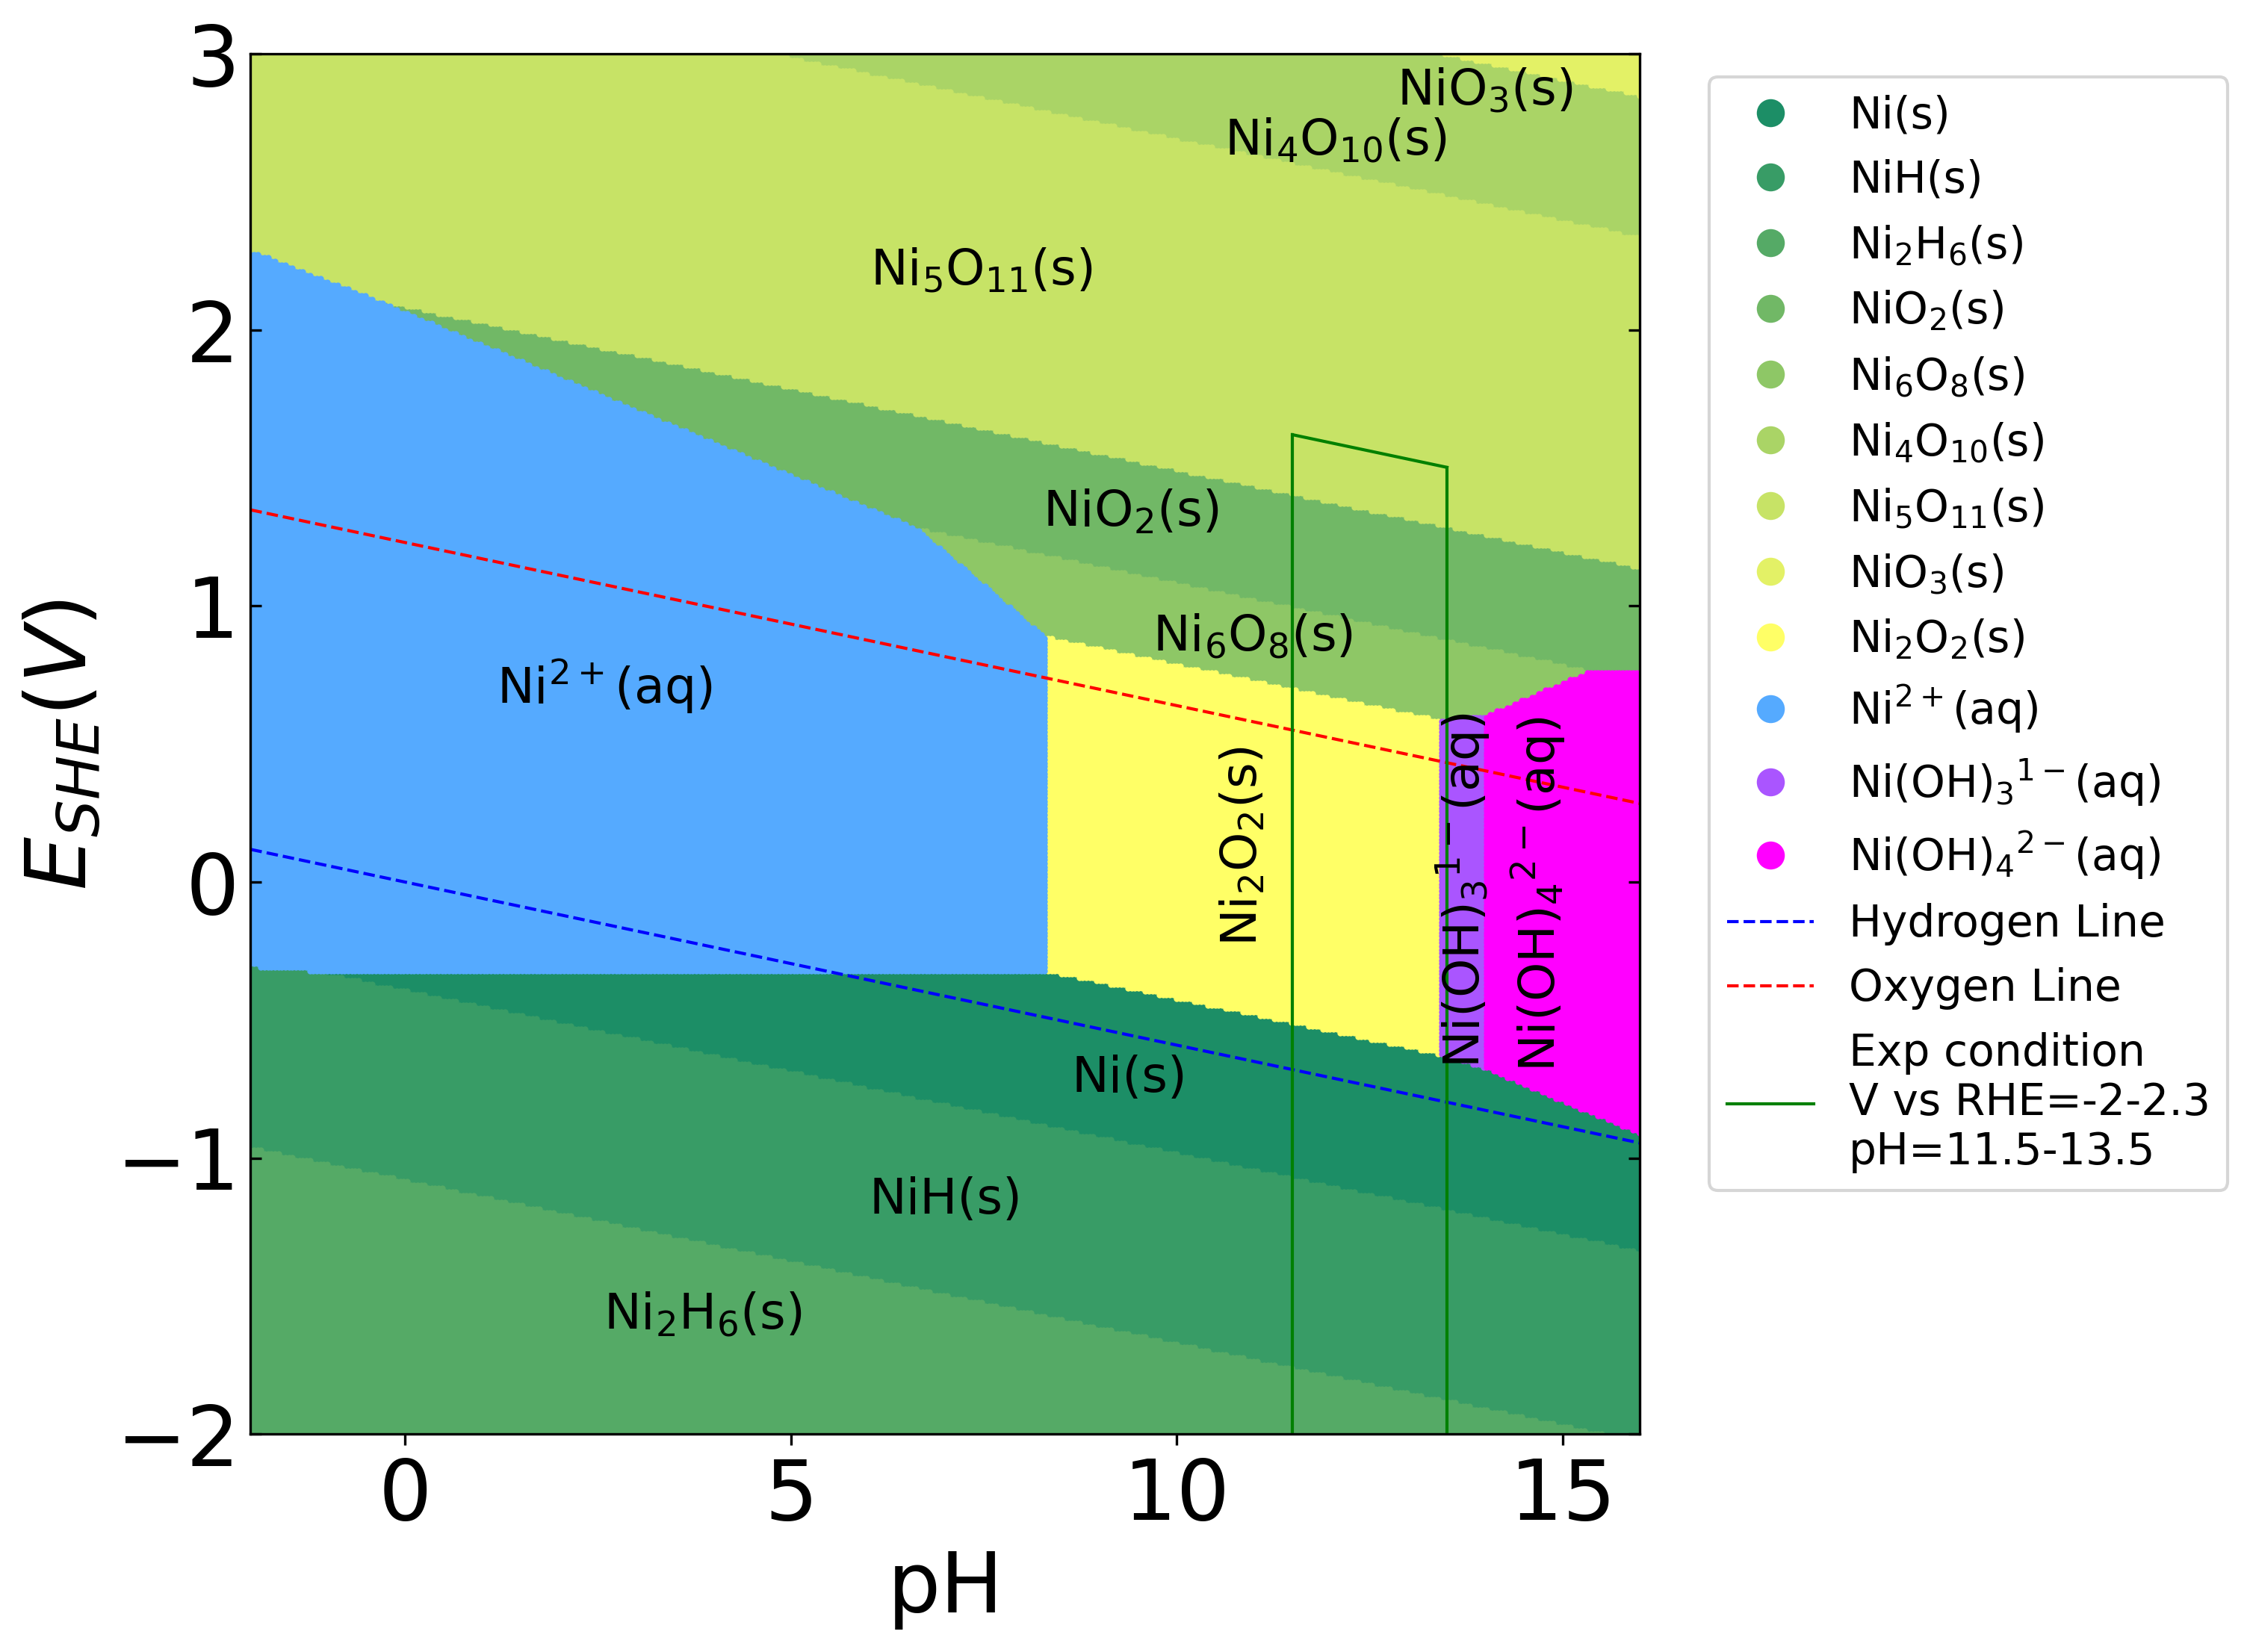
\includegraphics[width=\textwidth]{Figures/pourbaix_diagrams/Ni-NH3-H2O_activity=1e-04_[NH3]=0M_[Gly]=0M_[CN]=0.png}
        \par\medskip
    \end{subfigure}
    \begin{subfigure}[b]{0.3\textwidth}
        \subcaption{}\label{fig:Ni_Pourbaix_NH3_Gly}
        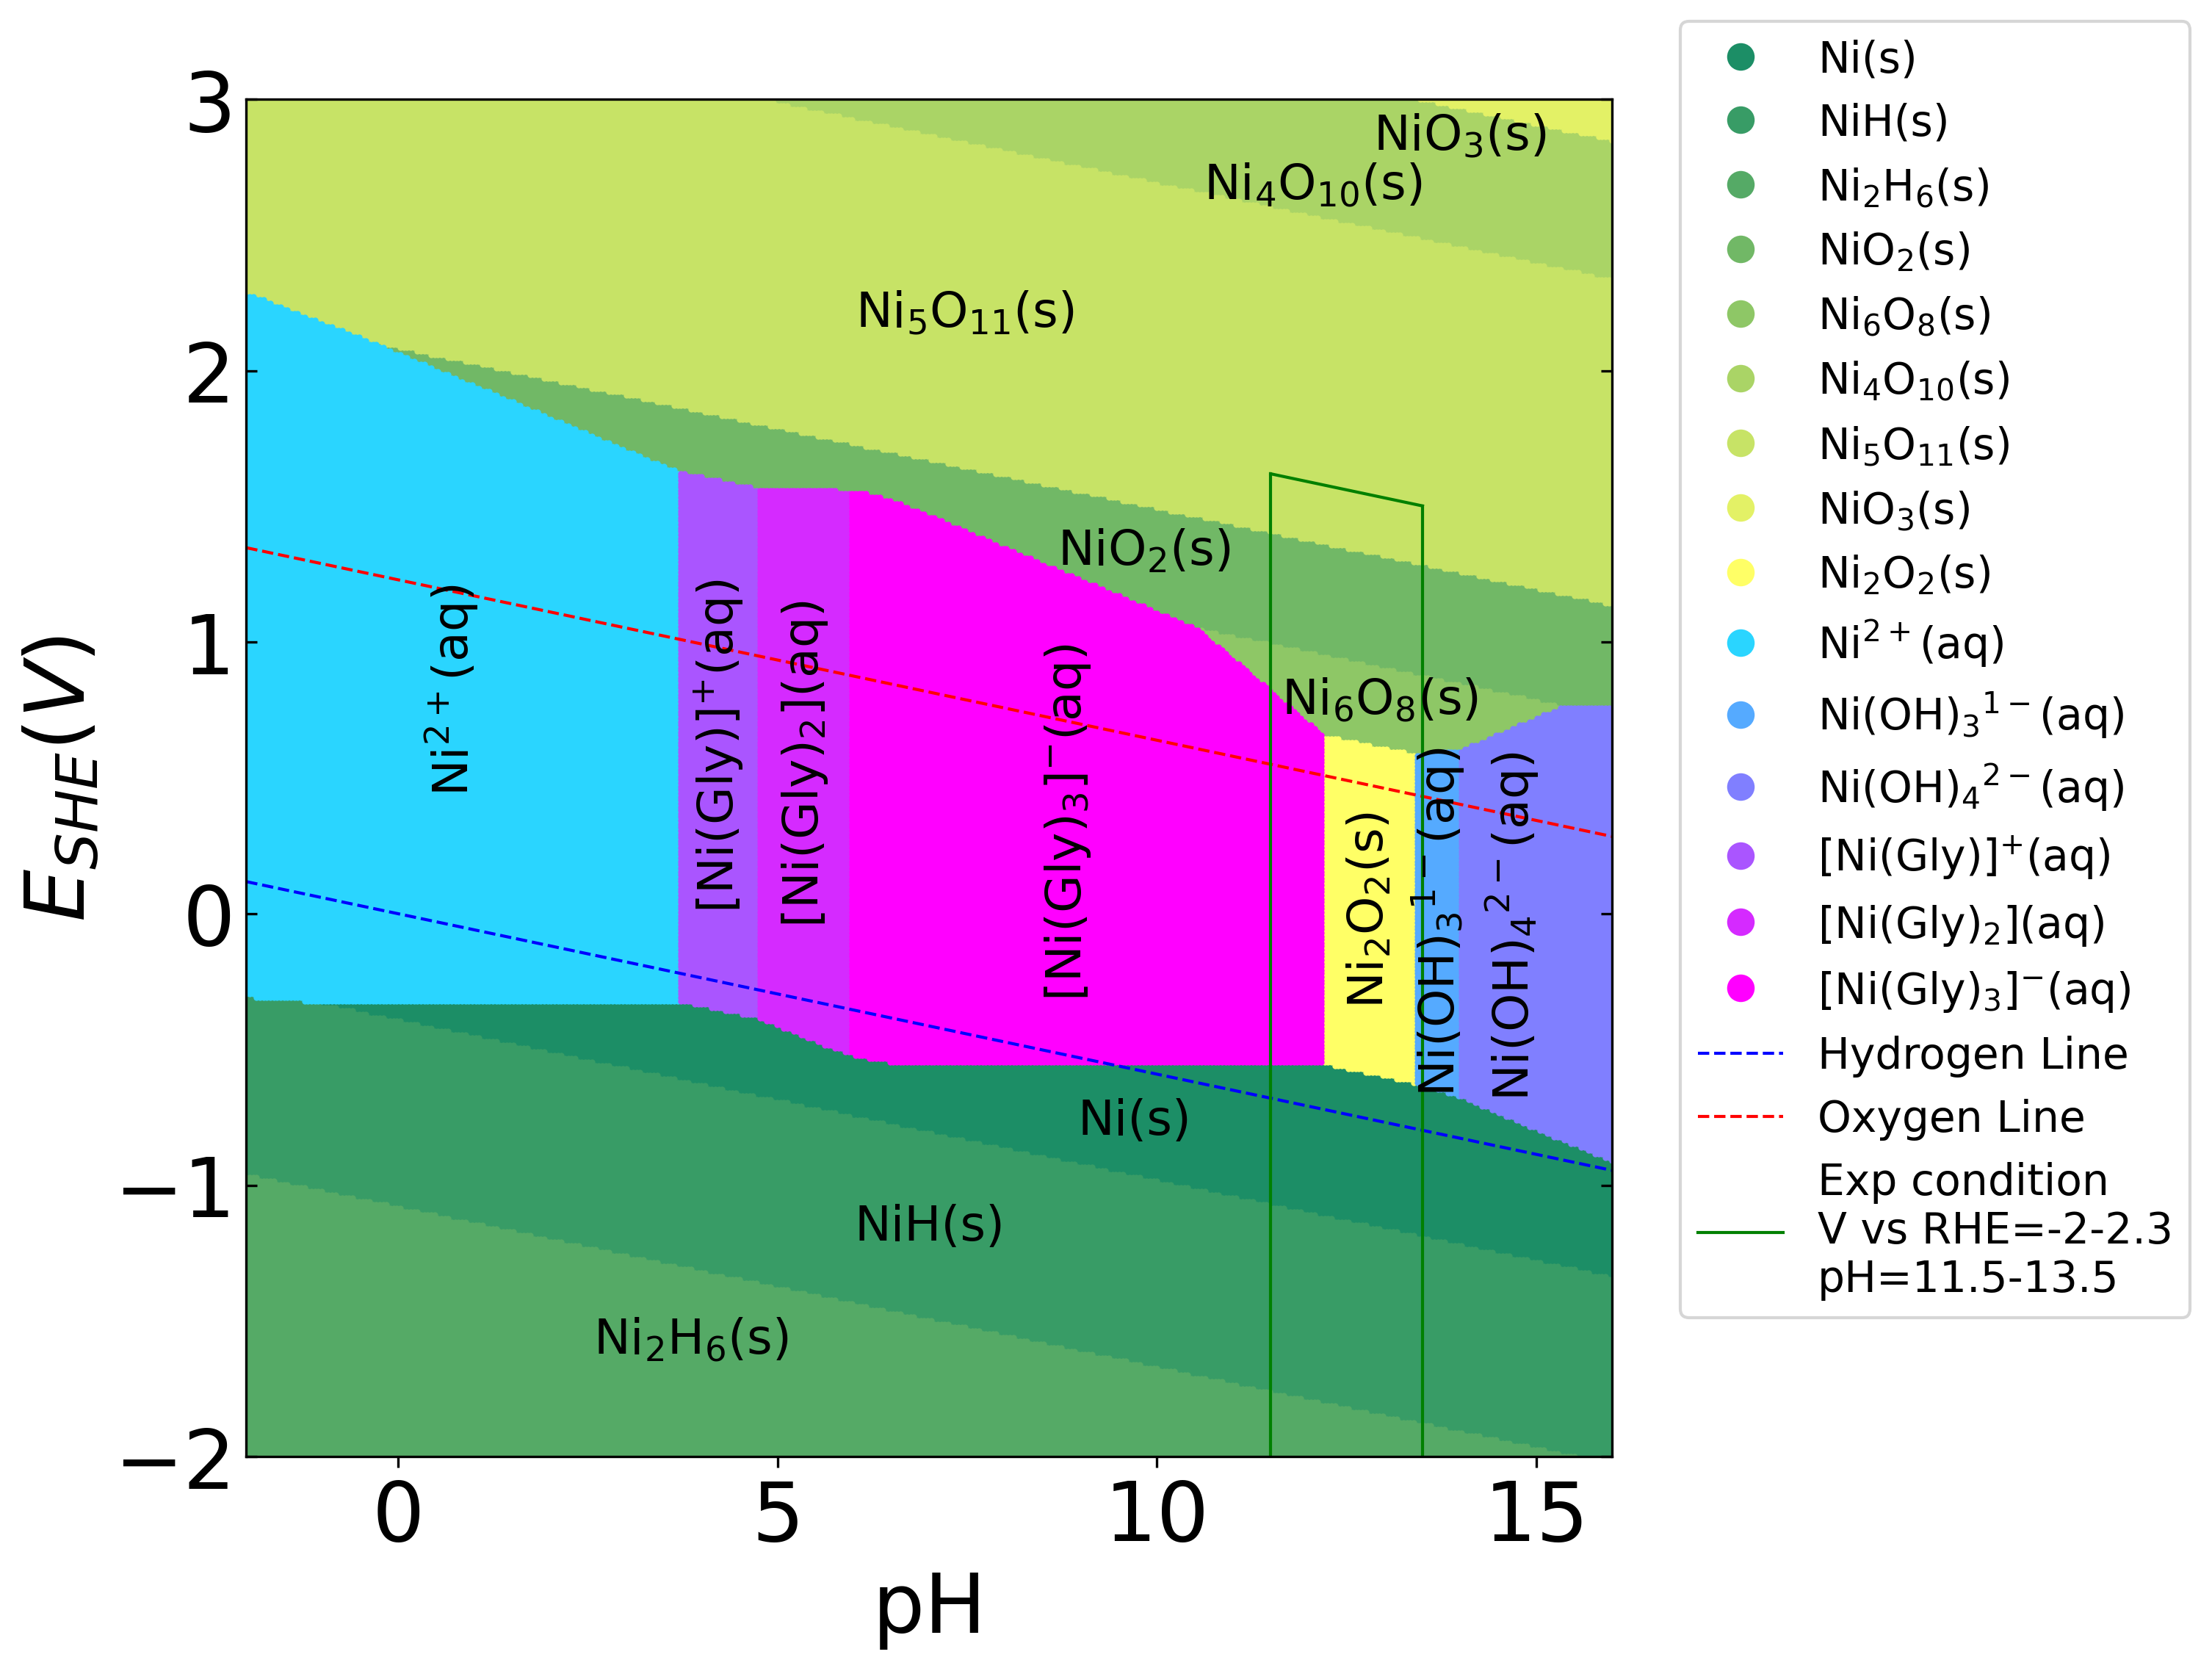
\includegraphics[width=\textwidth]{Figures/pourbaix_diagrams/Ni-NH3-H2O_activity=1e-04_[NH3]=0.02M_[Gly]=0.005M_[CN]=0.png}
        \par\medskip
    \end{subfigure}
    \begin{subfigure}[b]{0.3\textwidth}
        \subcaption{}\label{fig:Ni_Pourbaix_NH3_Gly_CN}
        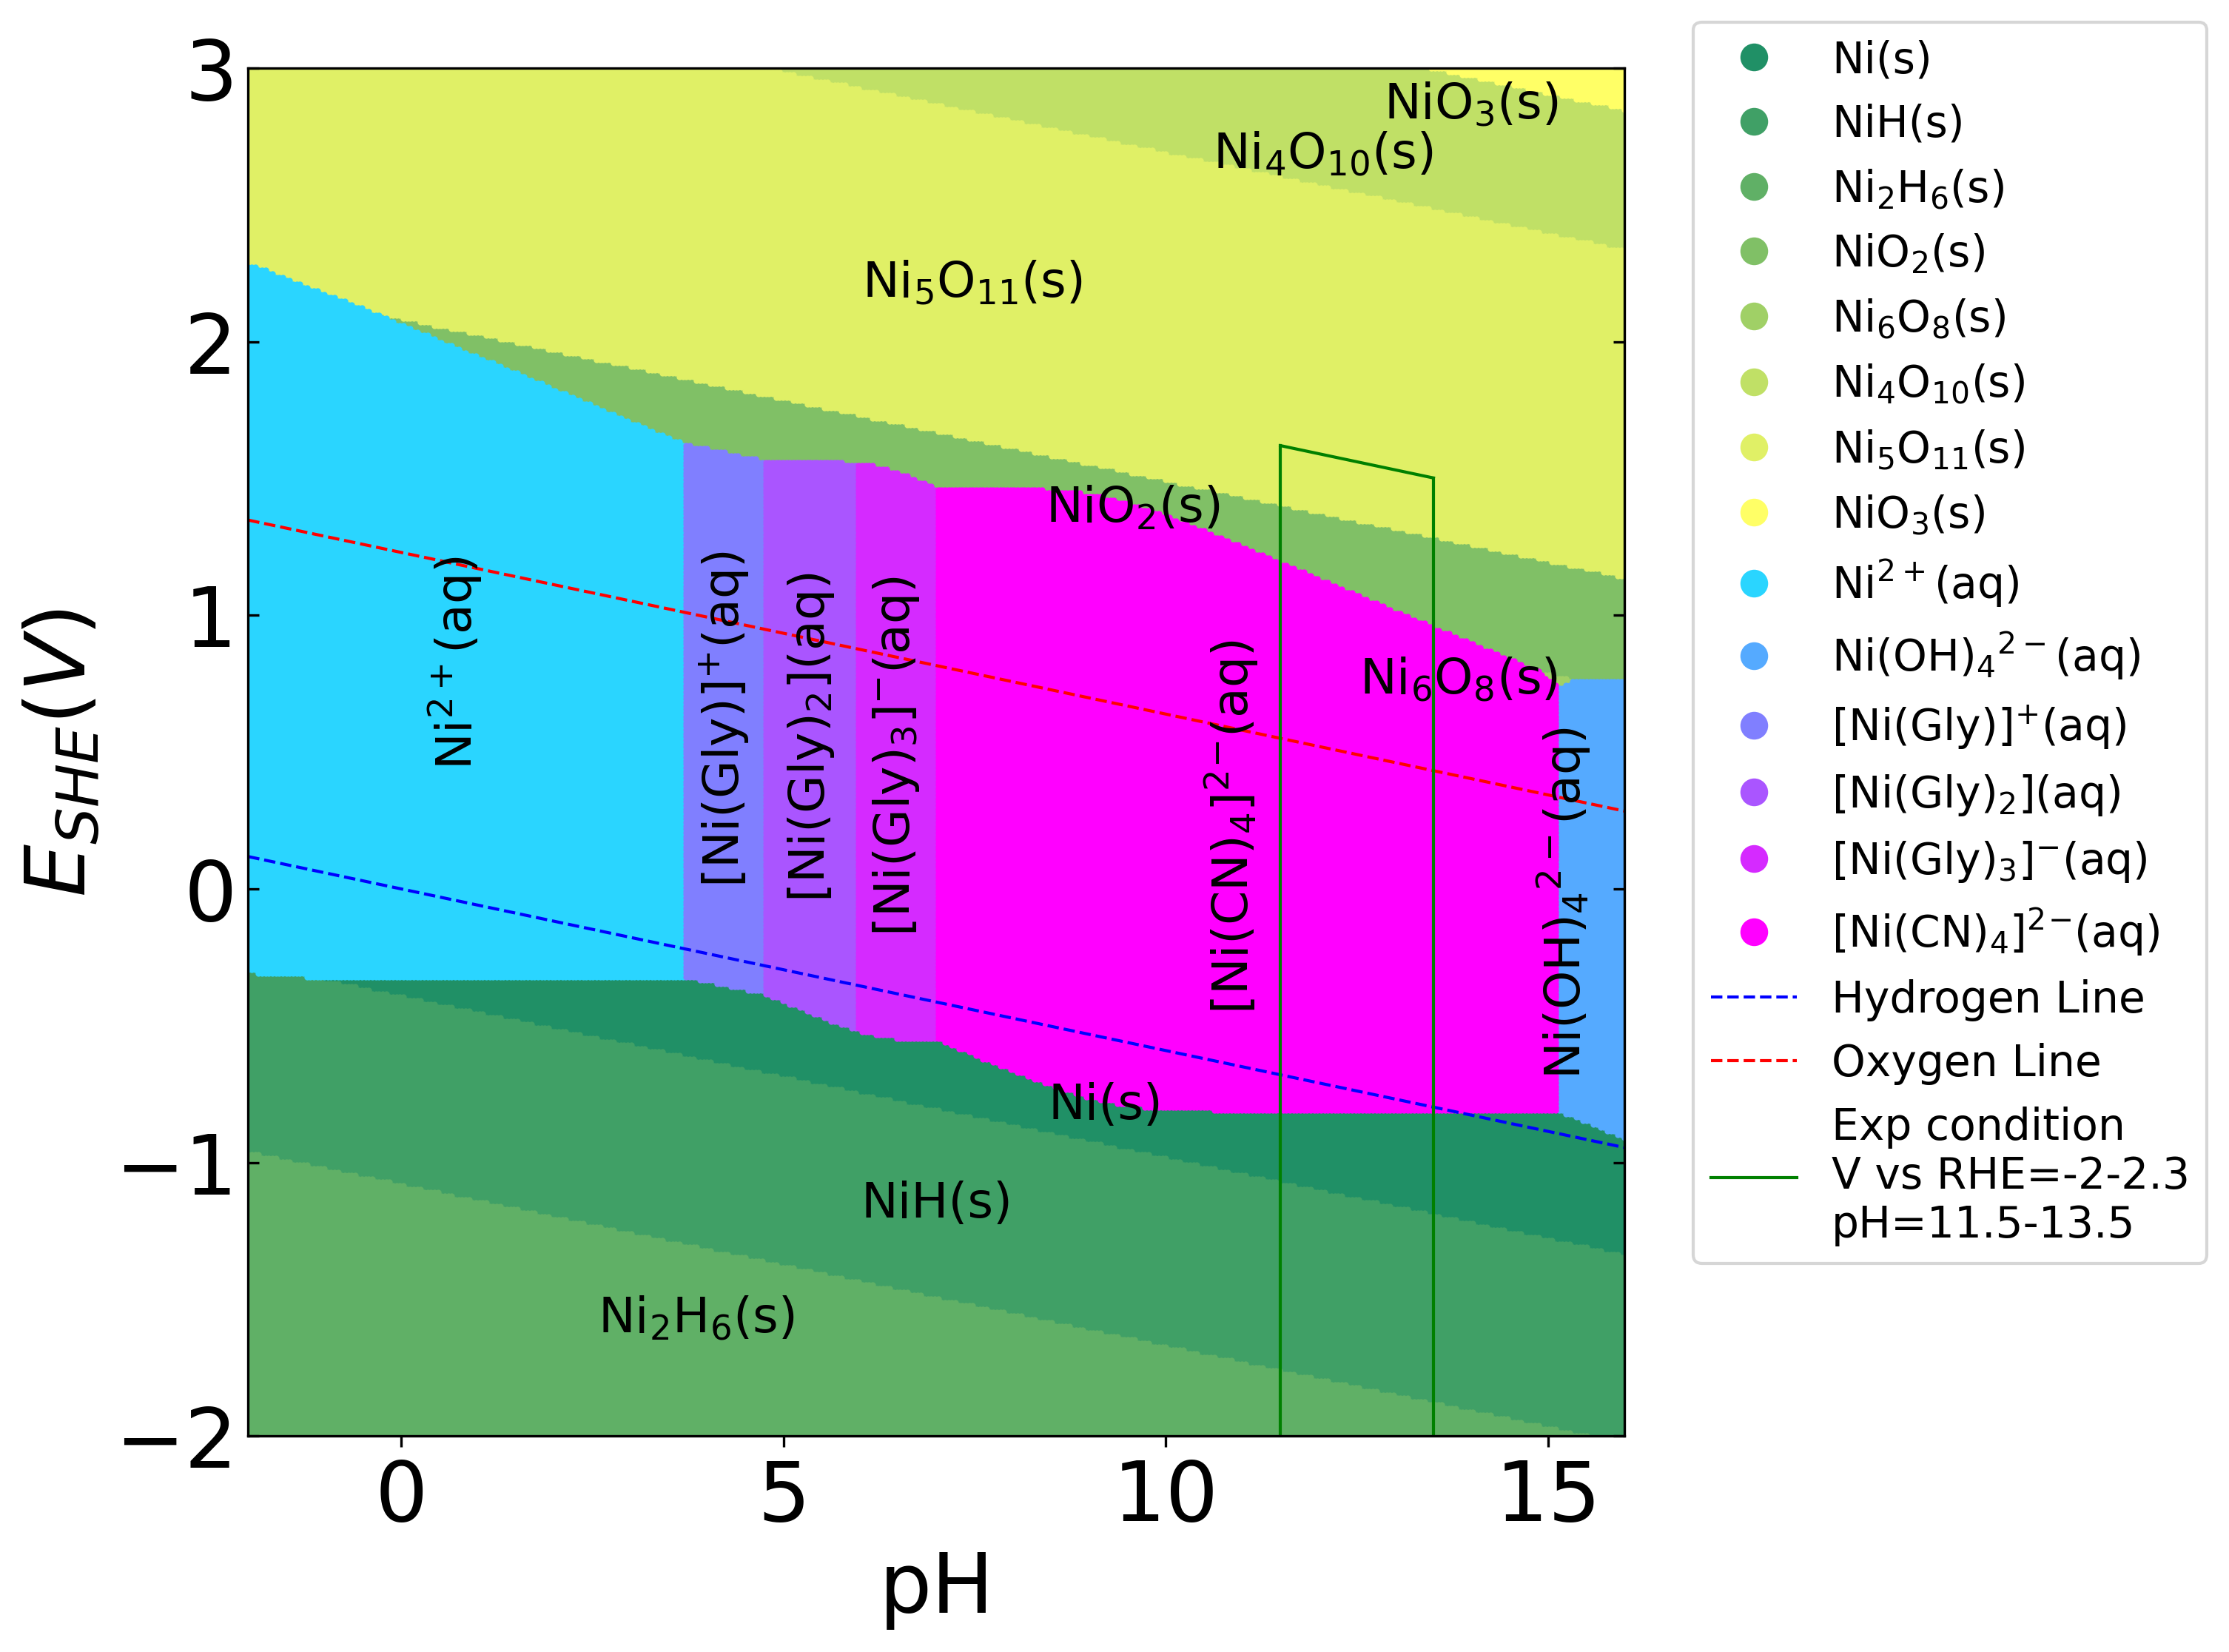
\includegraphics[width=\textwidth]{Figures/pourbaix_diagrams/Ni-NH3-H2O_activity=1e-04_[NH3]=0.02M_[Gly]=0.005M_[CN]=0.0001.png}
        \par\medskip   
    \end{subfigure}
    \caption{Ni Pourbaix diagrams, with $\text{ion activity}=\num{1e-4}$M, (a)\ce{H2O} only, (b)$[\ce{NH3}]_{initial}= 0.02$M, $[\text{Gly}]_{initial}=0.005$M, (c)$[\ce{NH3}]_{initial}= 0.02$M, $[\text{Gly}]_{initial}=0.005$M,  $[\ce{CN-}]_{initial}=\num{1e-4}$M. Green box indicates experimental condition at applied potential vs RHE = -2 to 2V, pH = 11.5 to 13.5.}
    \label{fig:Ni_Pourbaix}
\end{figure}
%%%%%%%%%%%%%%%%%%%%%%%%%%%%%%%%% Cu %%%%%%%%%%%%%%%%%%%%%%%%%%%%%%%%%
\begin{figure}[htbp]
    \centering
    \begin{subfigure}[b]{0.3\textwidth}
        \subcaption{}\label{fig:Cu_Pourbaix_H2O}
        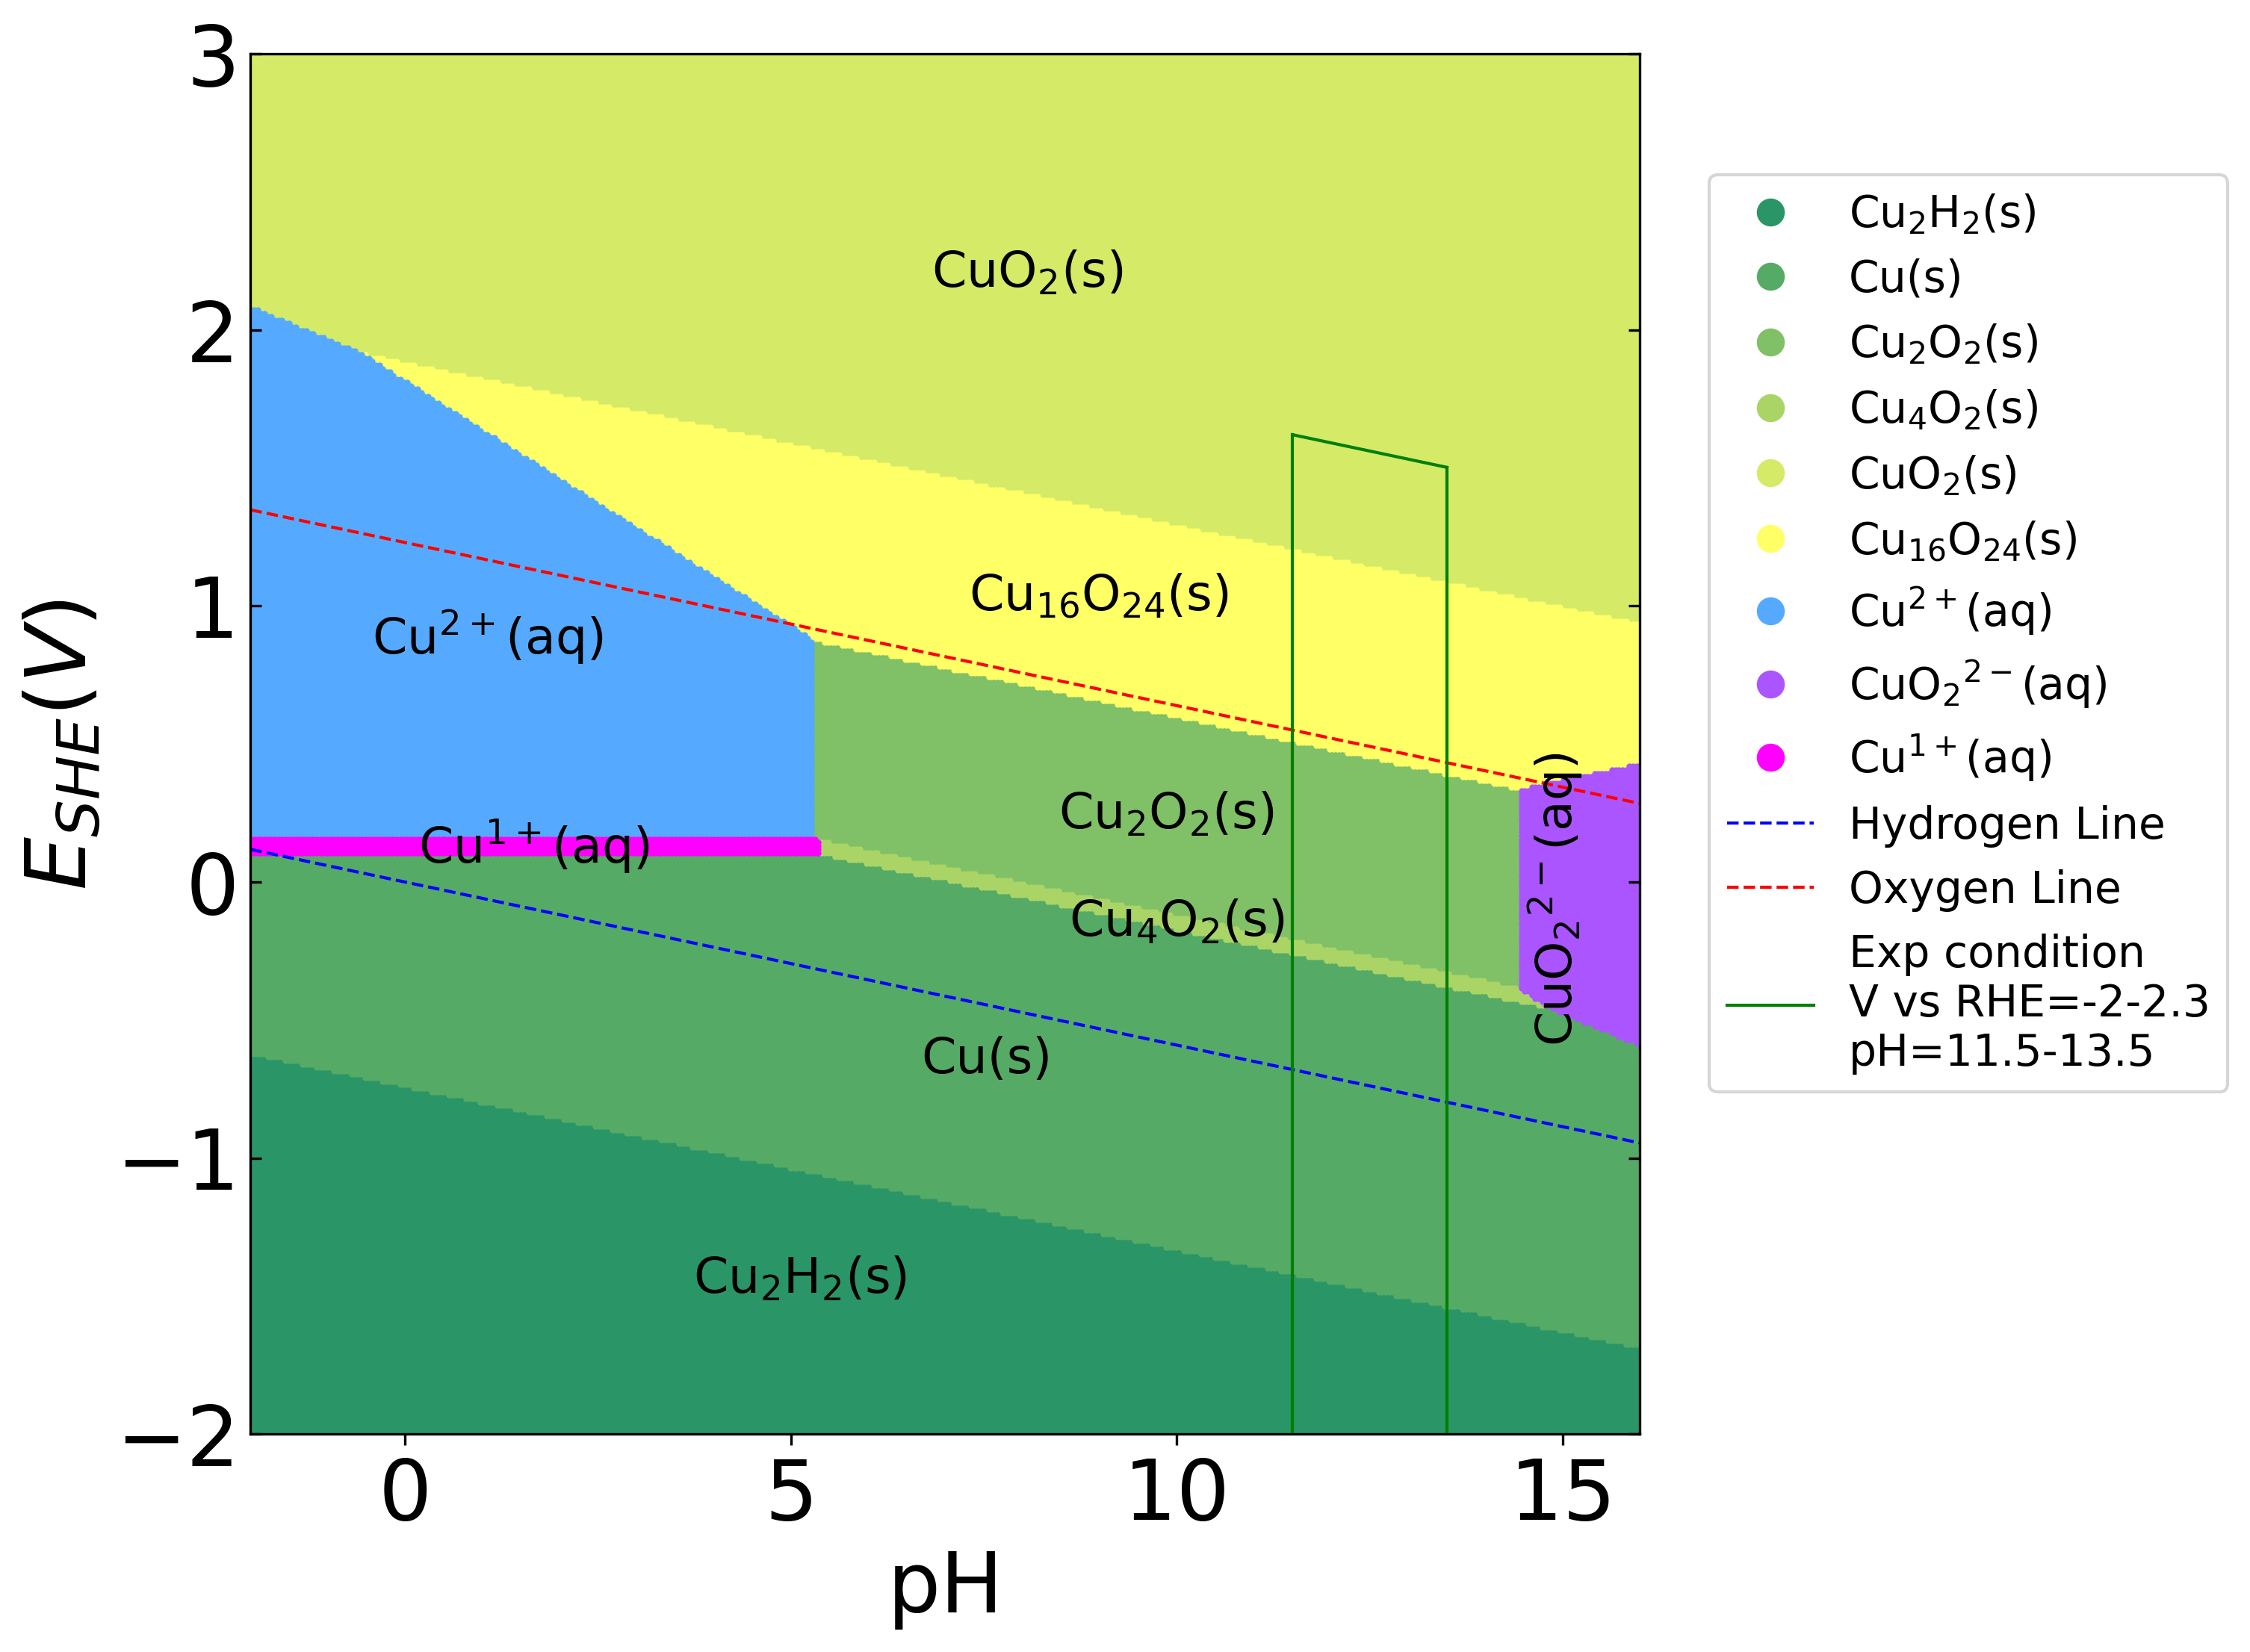
\includegraphics[width=\textwidth]{Figures/pourbaix_diagrams/Cu-NH3-H2O_activity=1e-04_[NH3]=0M_[Gly]=0M_[CN]=0.png}
        \par\medskip
    \end{subfigure}
    \begin{subfigure}[b]{0.3\textwidth}
        \subcaption{}\label{fig:Cu_Pourbaix_NH3_Gly}
        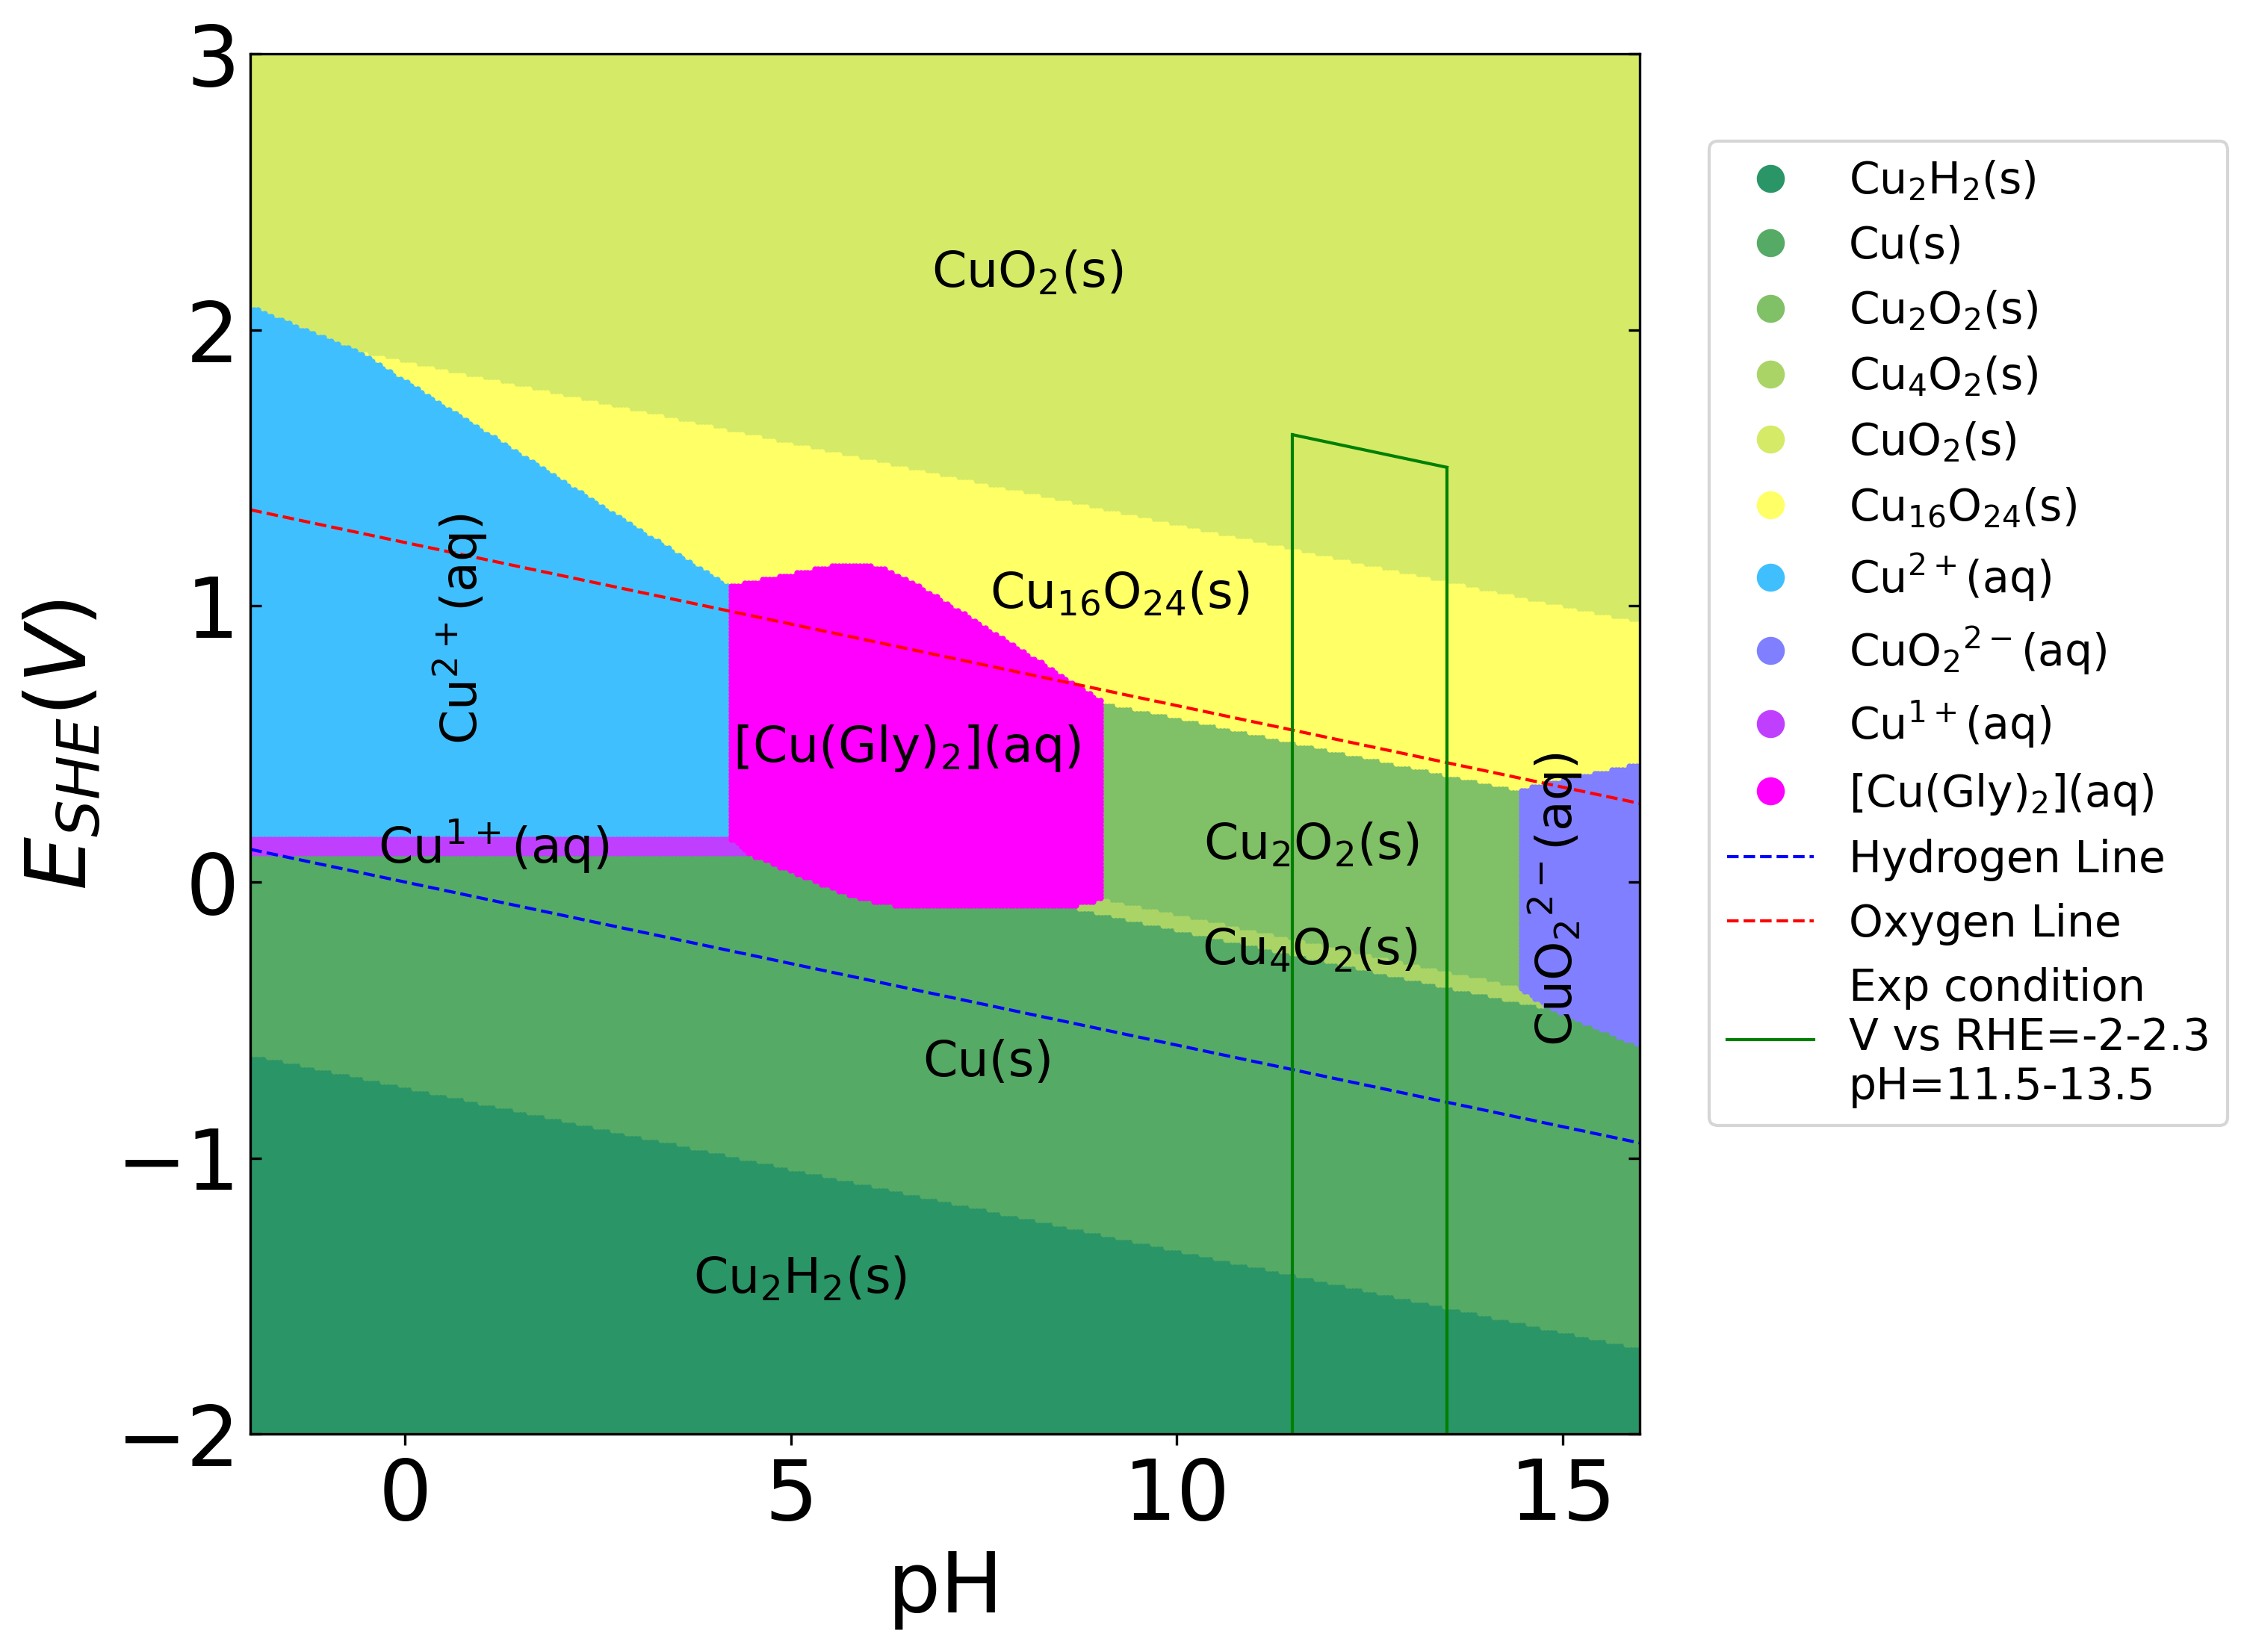
\includegraphics[width=\textwidth]{Figures/pourbaix_diagrams/Cu-NH3-H2O_activity=1e-04_[NH3]=0.02M_[Gly]=0.005M_[CN]=0.png}
        \par\medskip
    \end{subfigure}
    \begin{subfigure}[b]{0.3\textwidth}
        \subcaption{}\label{fig:Cu_Pourbaix_NH3_Gly_CN}
        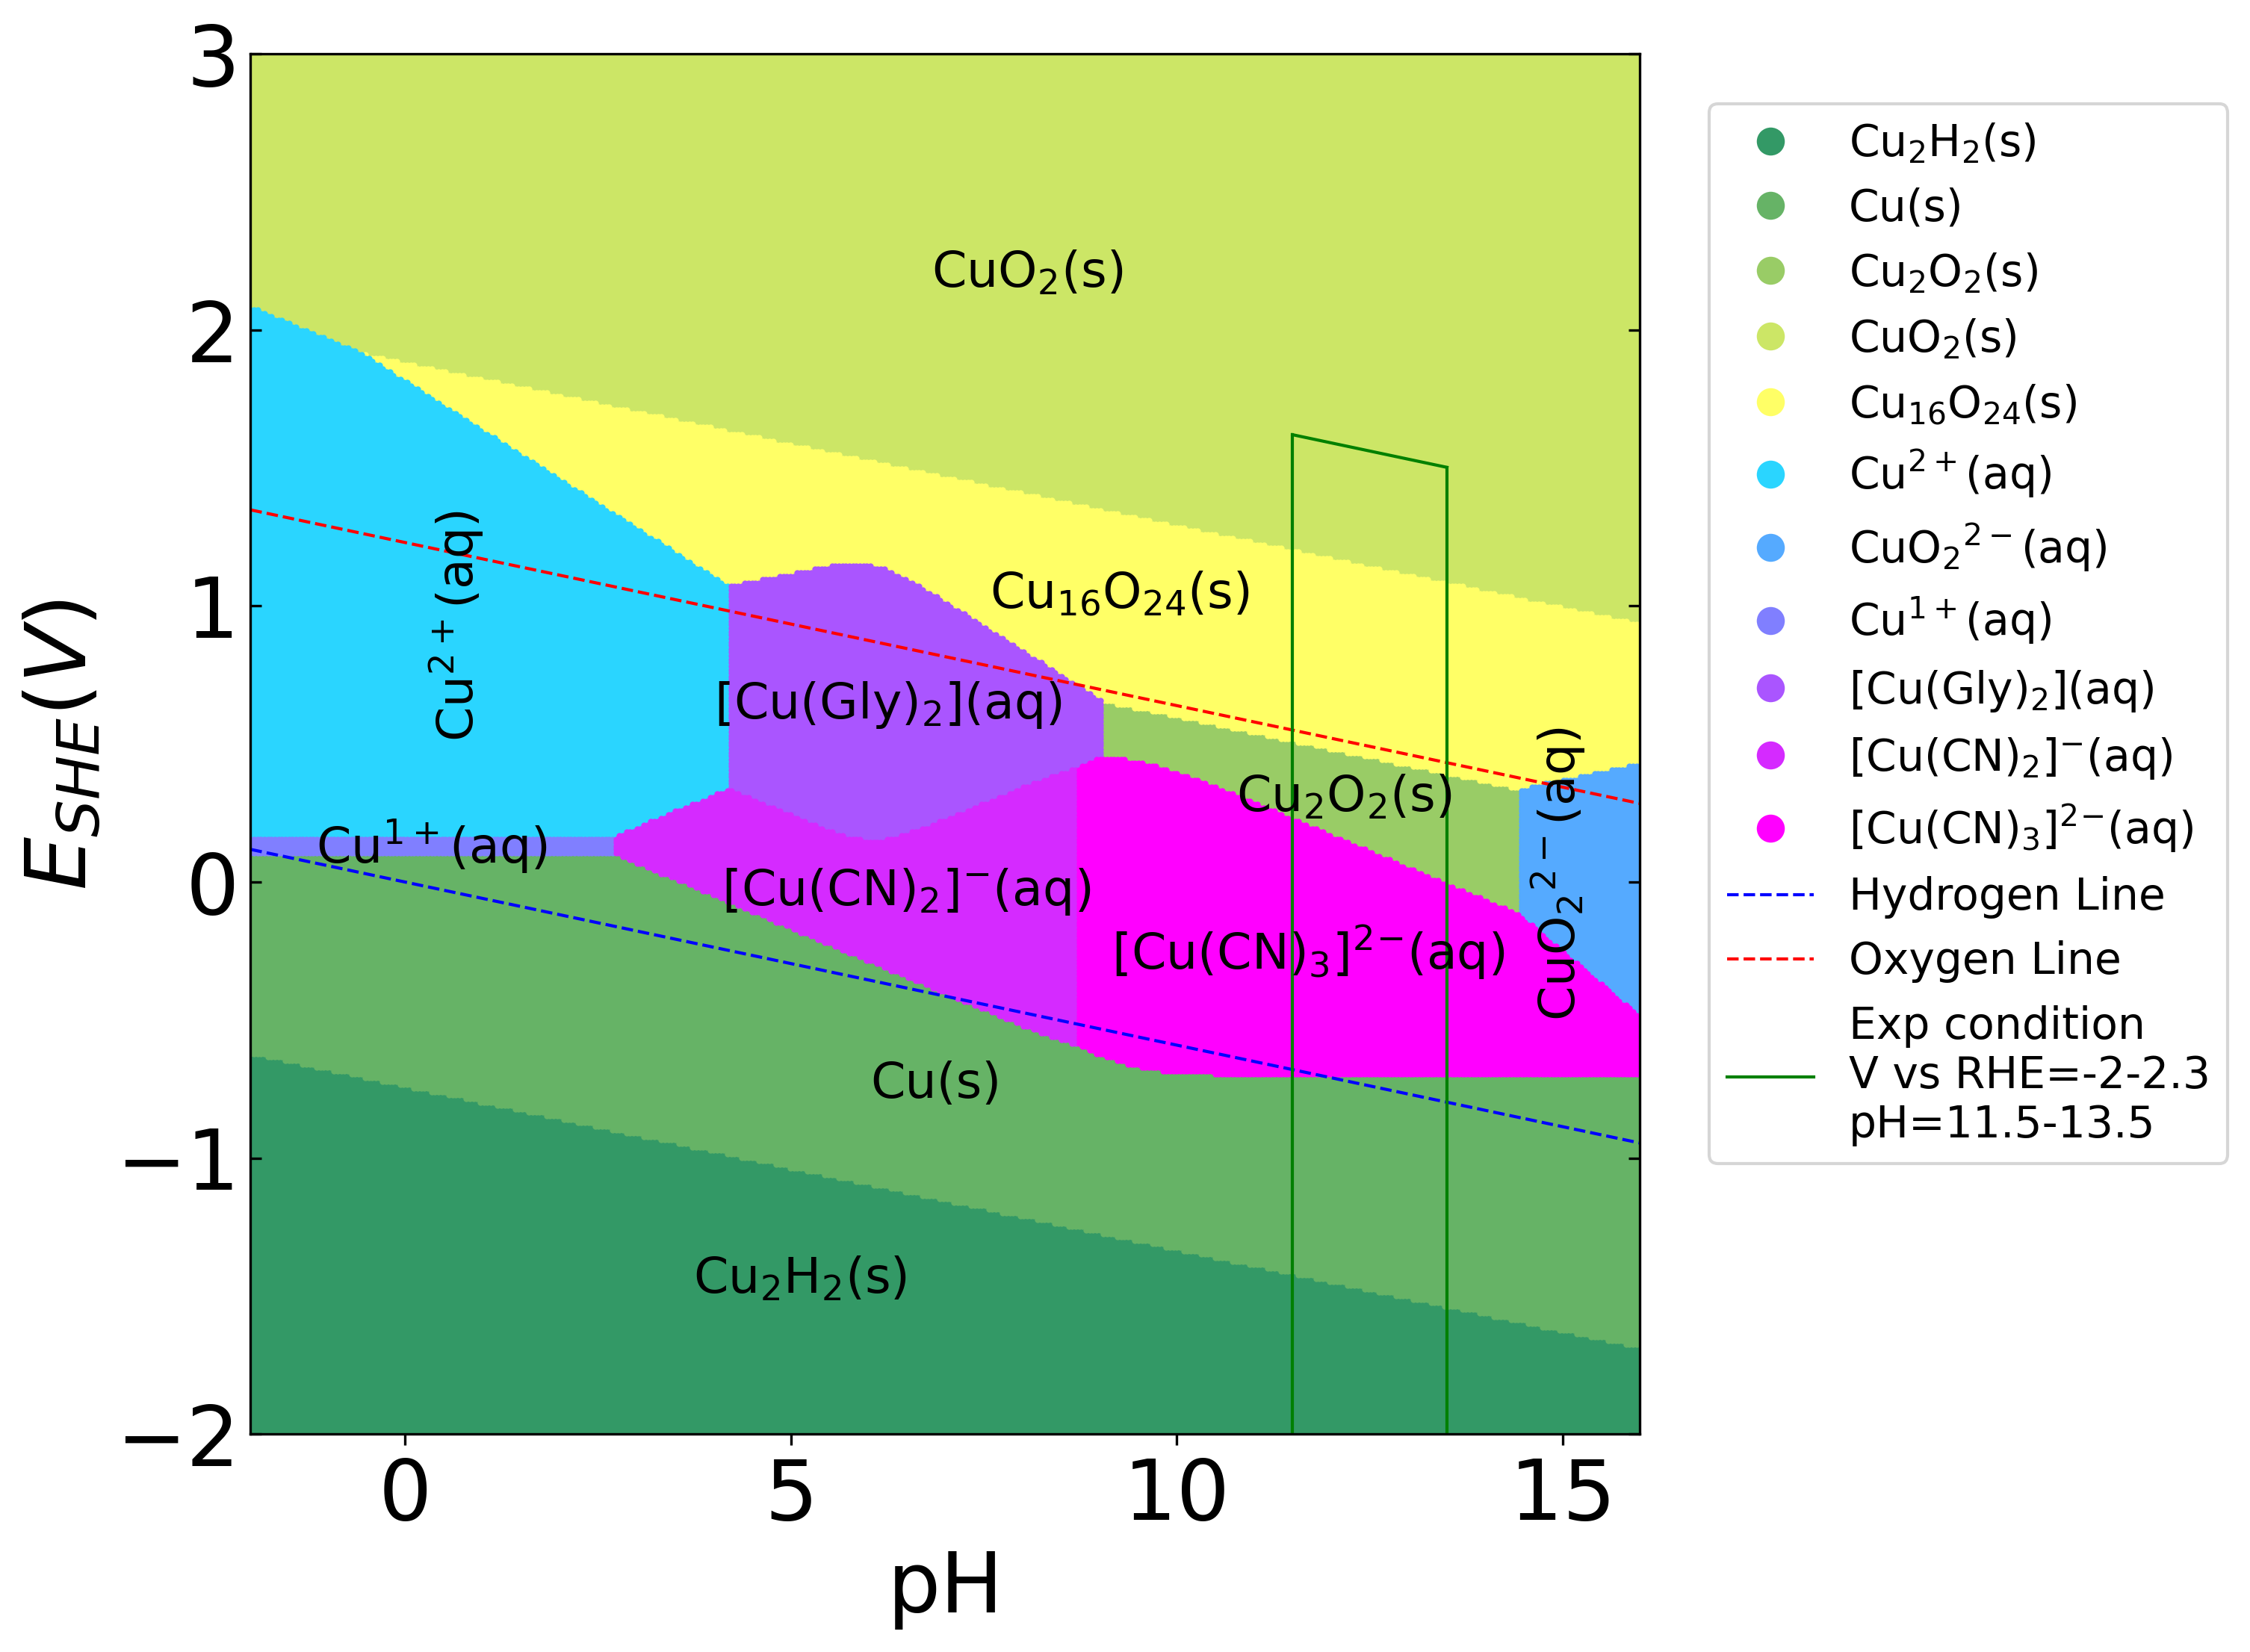
\includegraphics[width=\textwidth]{Figures/pourbaix_diagrams/Cu-NH3-H2O_activity=1e-04_[NH3]=0.02M_[Gly]=0.005M_[CN]=0.0001.png}
        \par\medskip   
    \end{subfigure}
    \caption{Cu Pourbaix diagrams, with $\text{ion activity}=\num{1e-4}$, (a)\ce{H2O} only, (b)$[\ce{NH3}]_{initial}= 0.02$M, $[\text{Gly}]_{initial}=0.005$M, (c)$[\ce{NH3}]_{initial}= 0.02$M, $[\text{Gly}]_{initial}=0.005$M,  $[\ce{CN-}]_{initial}=\num{1e-4}$M. Green box indicates experimental condition at applied potential vs RHE = -2 to 2V, pH = 11.5 to 13.5.}
    \label{fig:Cu_Pourbaix}
\end{figure}
%%%%%%%%%%%%%%%%%%%%%%%%%%%%%%%%% Pd %%%%%%%%%%%%%%%%%%%%%%%%%%%%%%%%%
\begin{figure}[htbp]
    \centering
    \begin{subfigure}[b]{0.45\textwidth}
        \subcaption{}\label{fig:Pd_Pourbaix_NH3_Gly}
        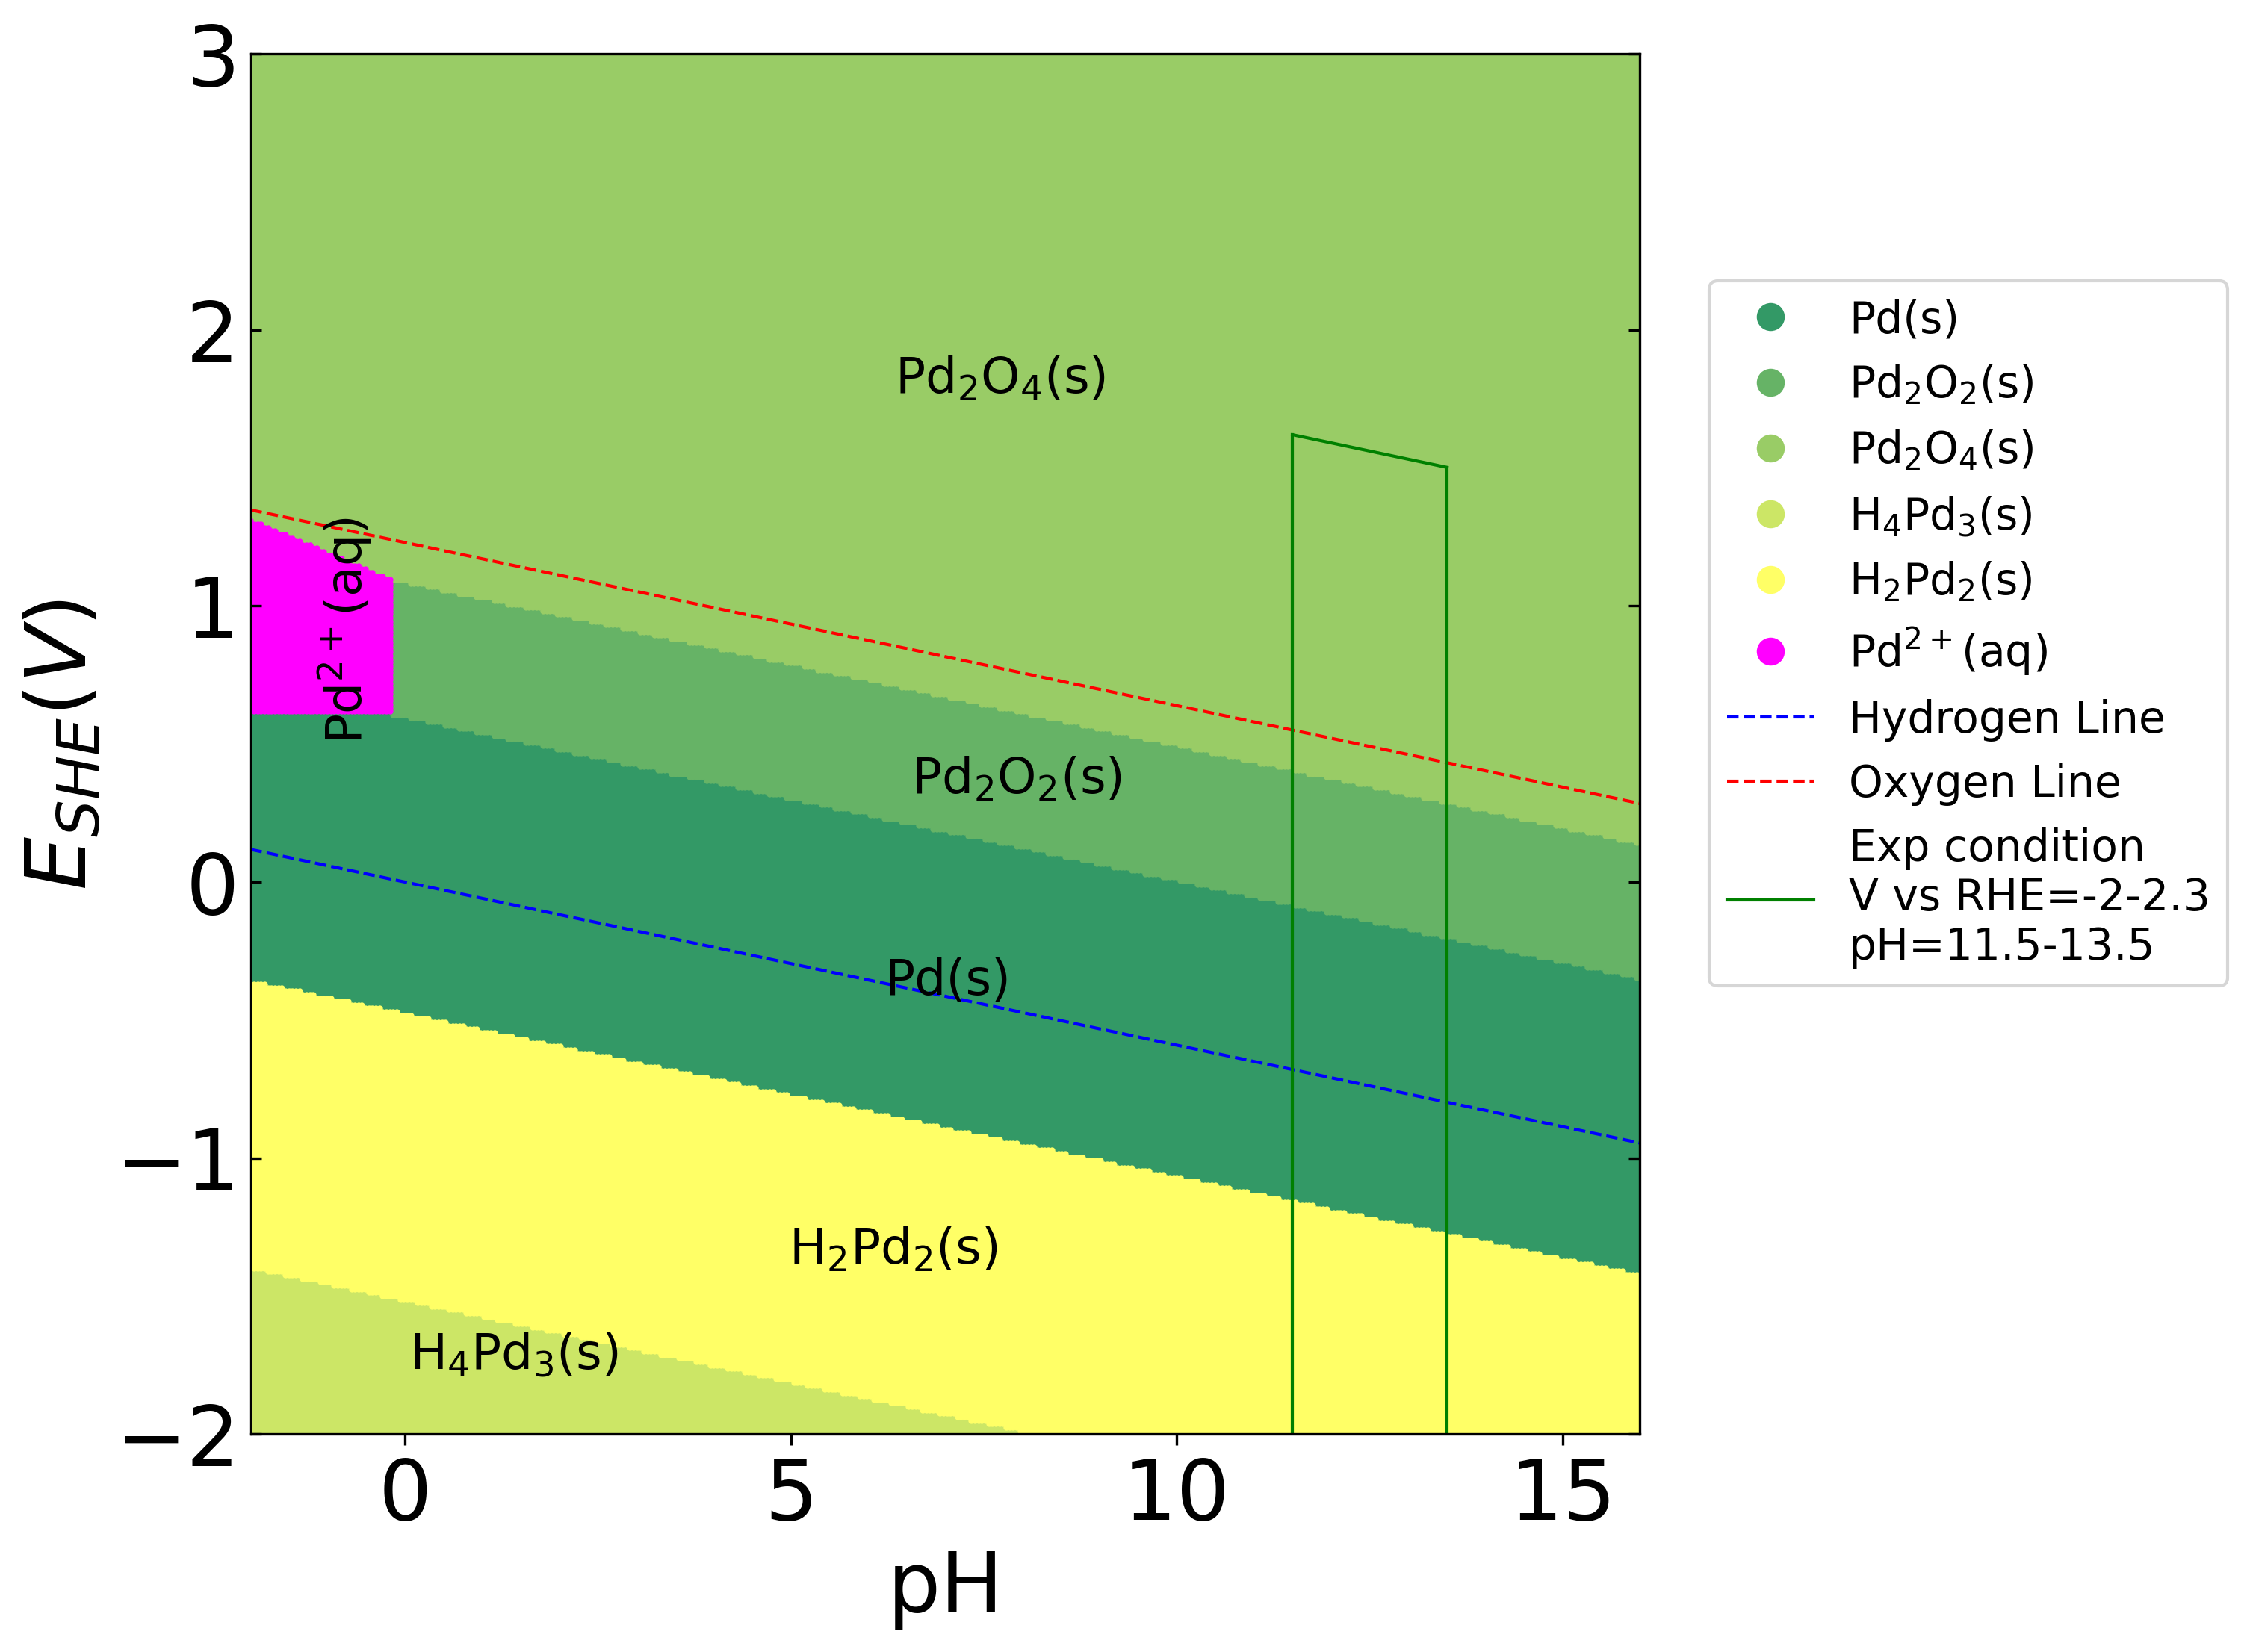
\includegraphics[width=\textwidth]{Figures/pourbaix_diagrams/Pd-NH3-H2O_activity=1e-04_[NH3]=0.02M_[Gly]=0.005M_[CN]=0.png}
        \par\medskip
    \end{subfigure}
    \begin{subfigure}[b]{0.45\textwidth}
        \subcaption{}\label{fig:Pd_Pourbaix_NH3_Gly_CN}
        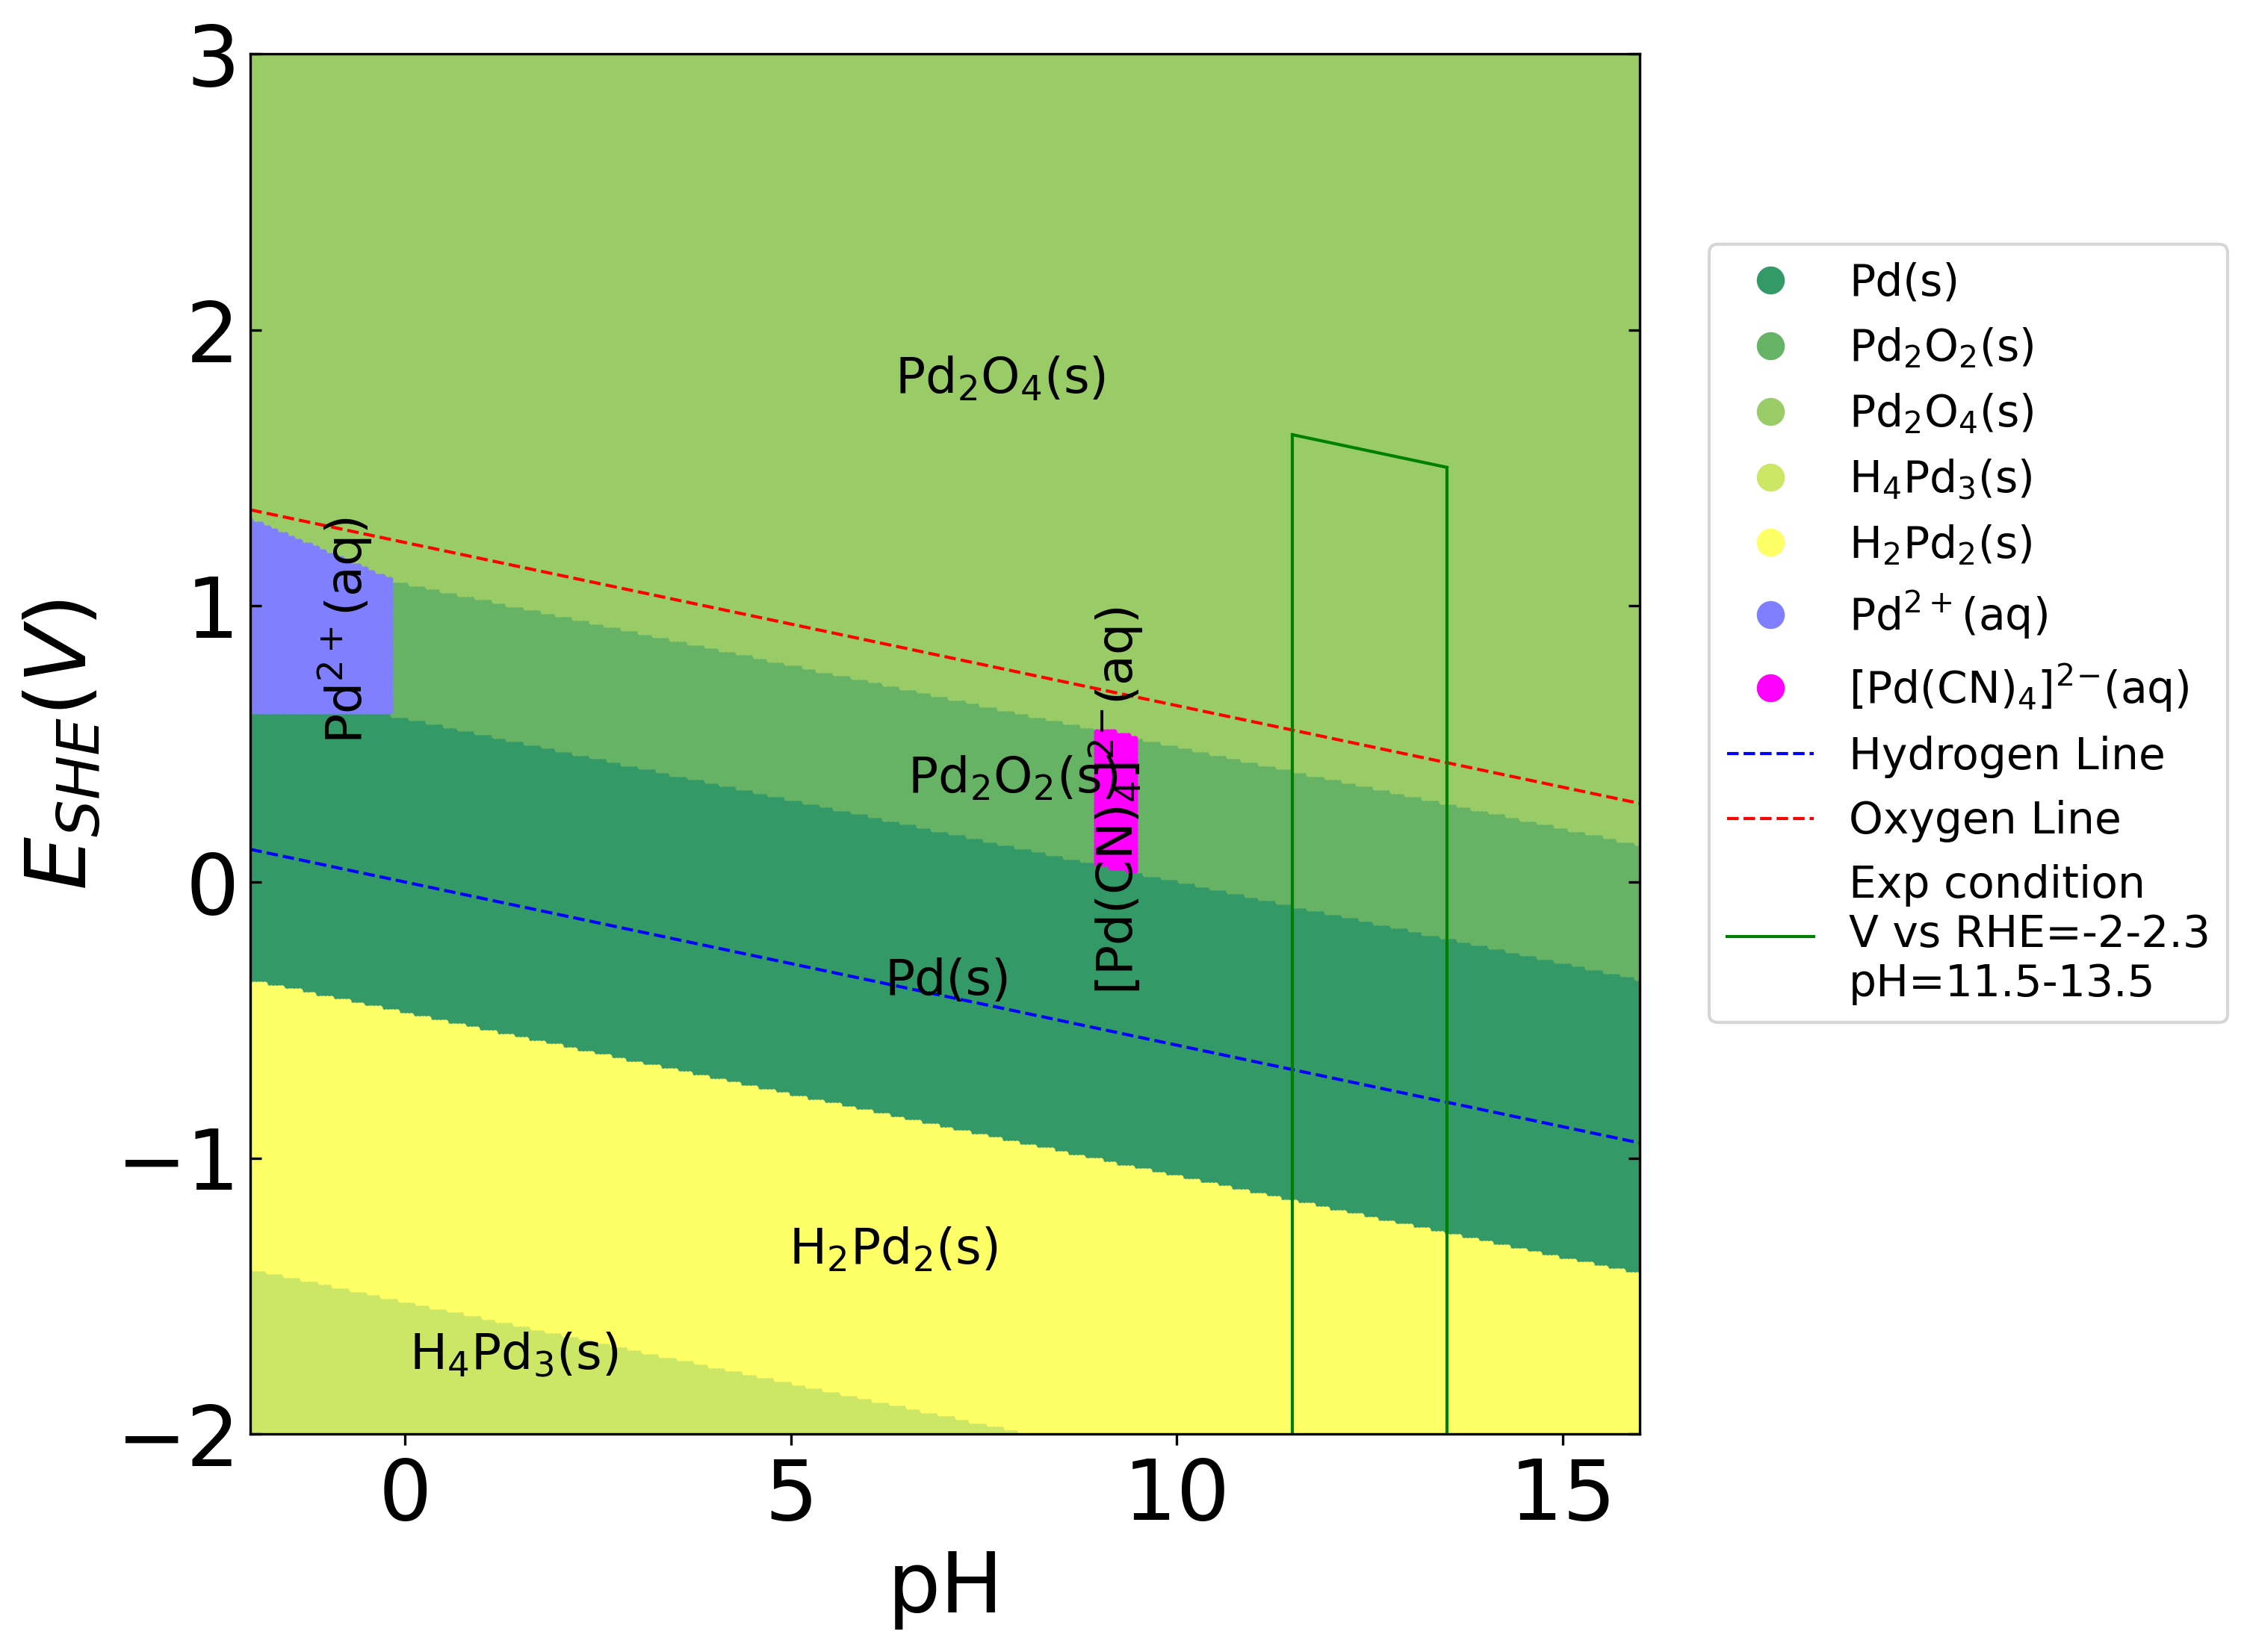
\includegraphics[width=\textwidth]{Figures/pourbaix_diagrams/Pd-NH3-H2O_activity=1e-04_[NH3]=0.02M_[Gly]=0.005M_[CN]=0.0001.png}
        \par\medskip   
    \end{subfigure}

    \caption{Pd Pourbaix diagrams, with $\text{ion activity}=\num{1e-4}$, (a)$[\ce{NH3}]_{initial}= 0.02$M, $[\text{Gly}]_{initial}=0.005$M, (b)$[\ce{NH3}]_{initial}= 0.02$M, $[\text{Gly}]_{initial}=0.005$M,  $[\ce{CN-}]_{initial}=\num{1e-4}$M. Green box indicates experimental condition at applied potential vs RHE = -2 to 2V, pH = 11.5 to 13.5.}
    \label{fig:Pd_Pourbaix}
\end{figure}
% %%%%%%%%%%%%%%%%%%%%%%%%%%%%%%%%% Pt %%%%%%%%%%%%%%%%%%%%%%%%%%%%%%%%%
% \begin{figure}[htbp]
%     \centering
%     \begin{subfigure}[b]{0.3\textwidth}
%         \subcaption{}\label{fig:Pt_Pourbaix_H2O}
%         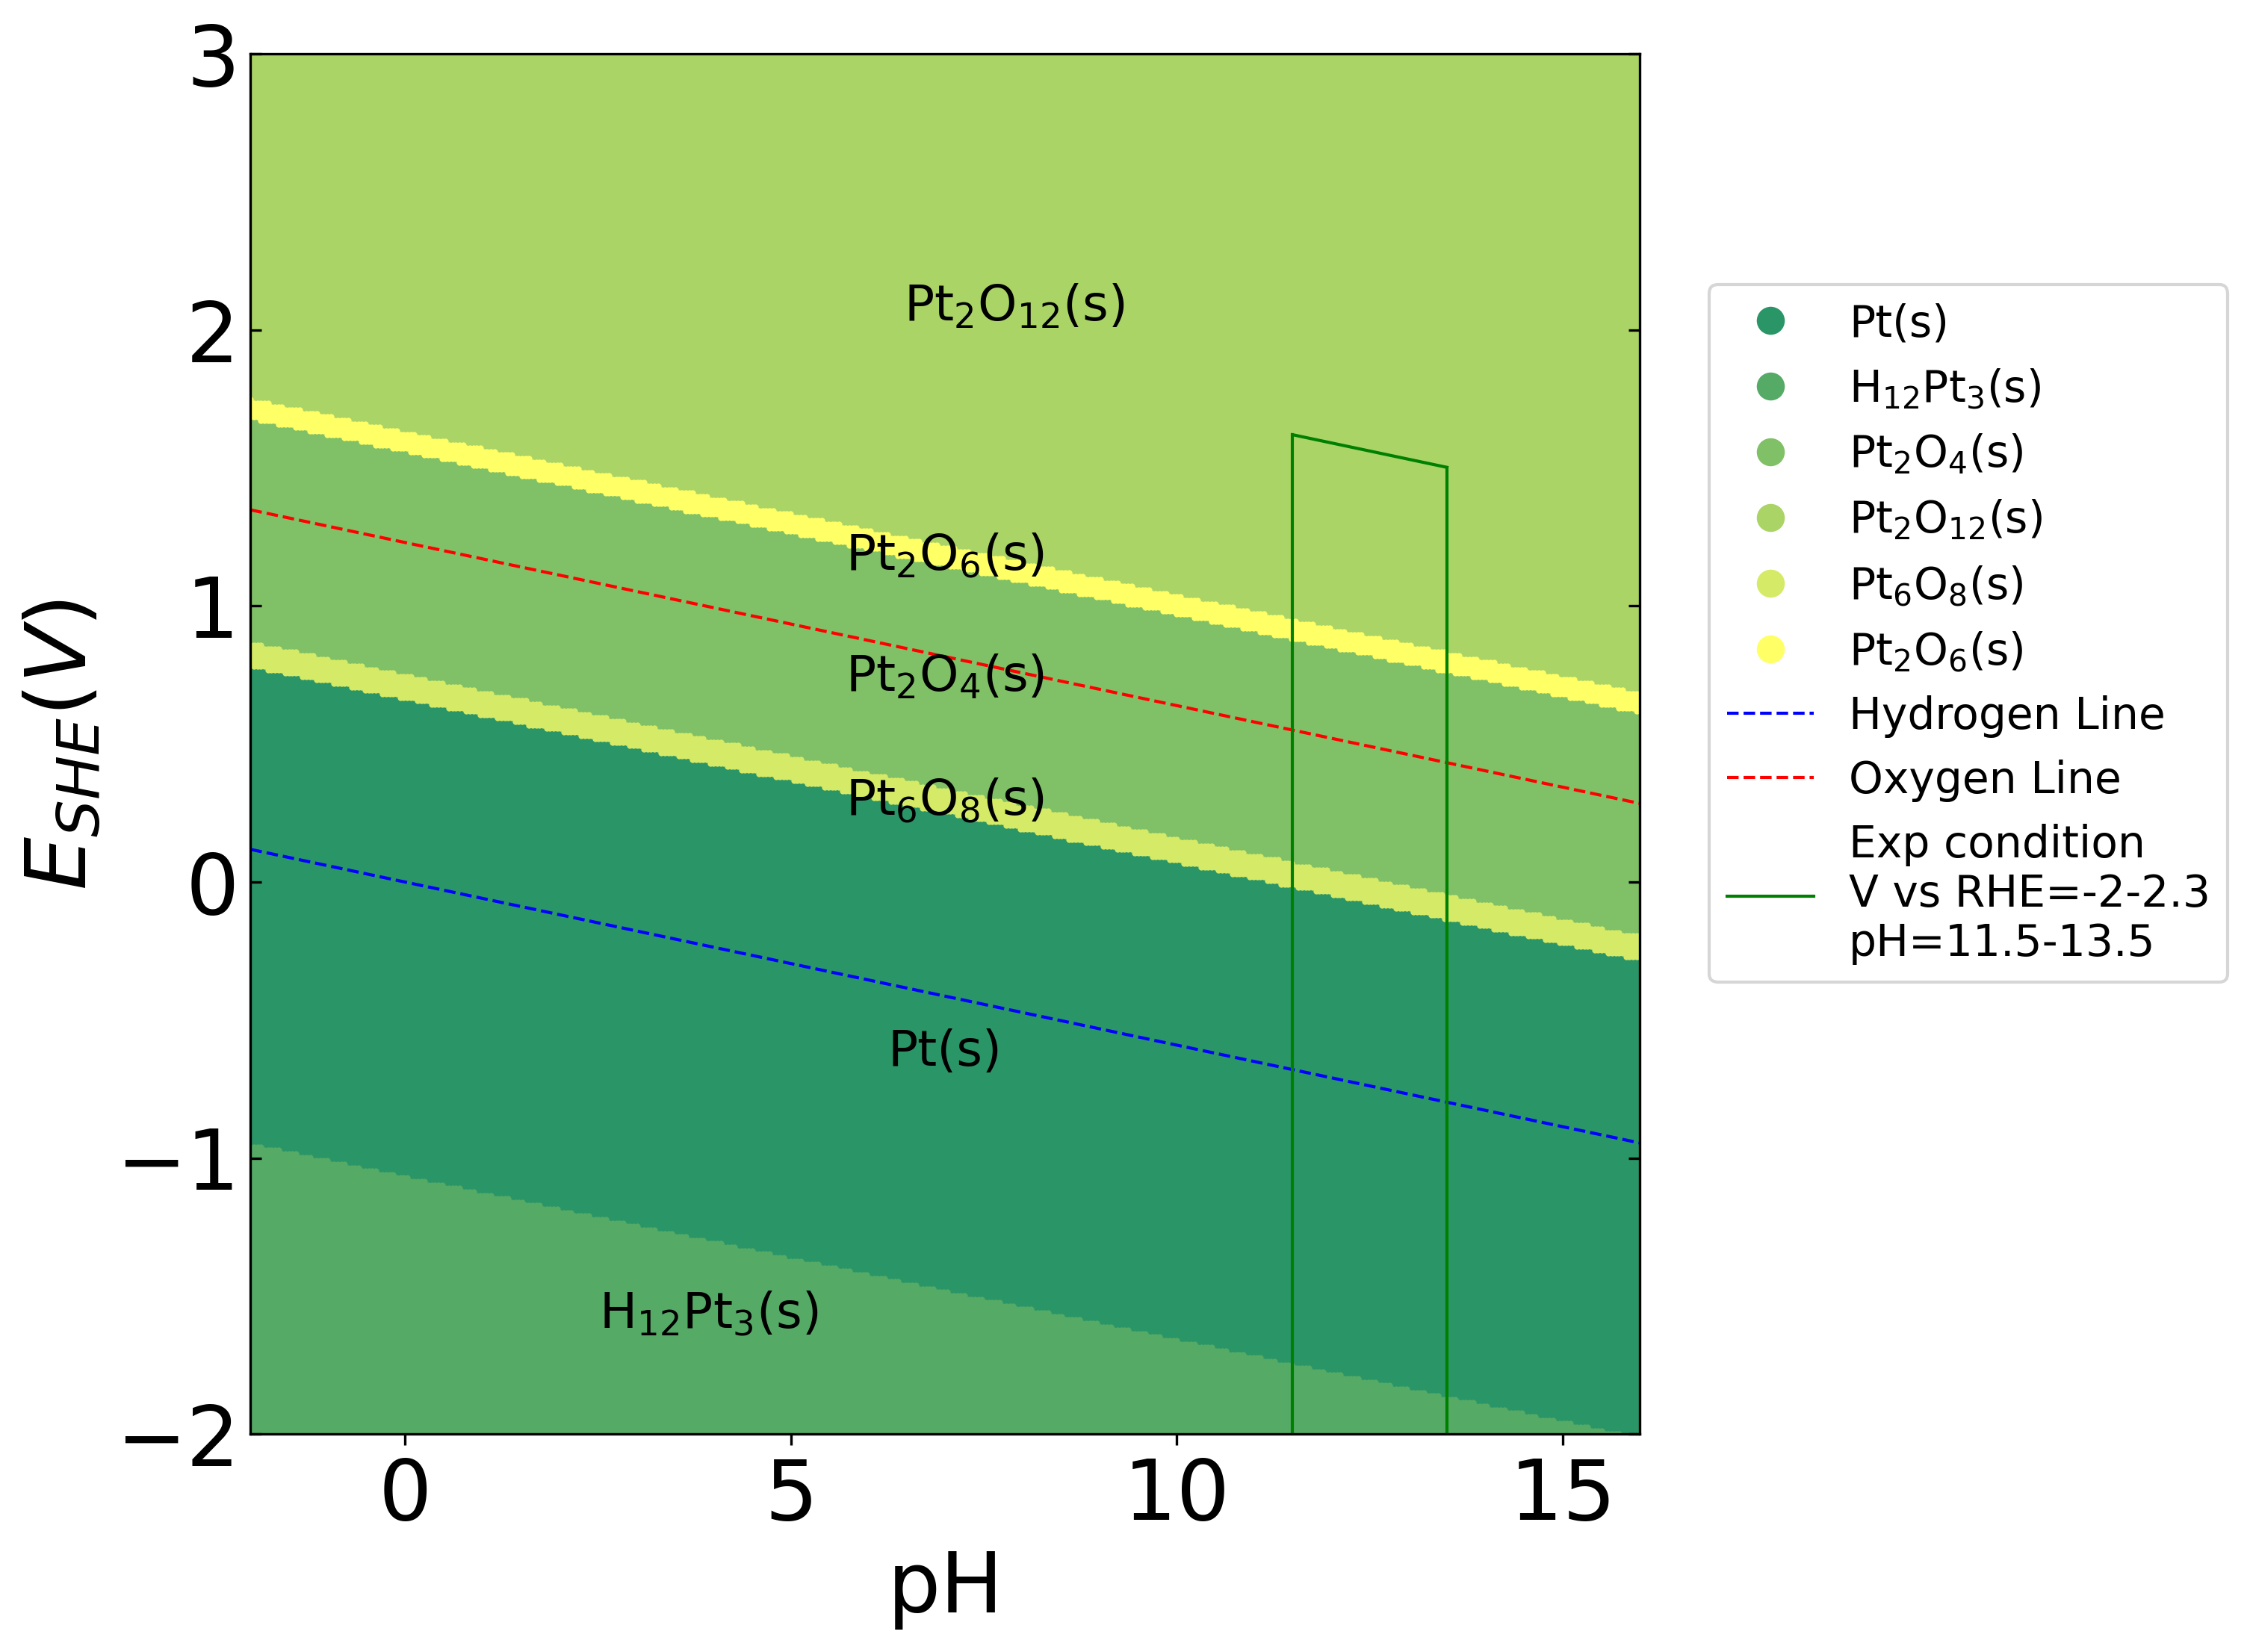
\includegraphics[width=\textwidth]{Figures/pourbaix_diagrams/Pt-NH3-H2O_activity=1e-04_[NH3]=0M_[Gly]=0M_[CN]=0.png}
%         \par\medskip
%     \end{subfigure}
%     \begin{subfigure}[b]{0.3\textwidth}
%         \subcaption{}\label{fig:Pt_Pourbaix_NH3_Gly}
%         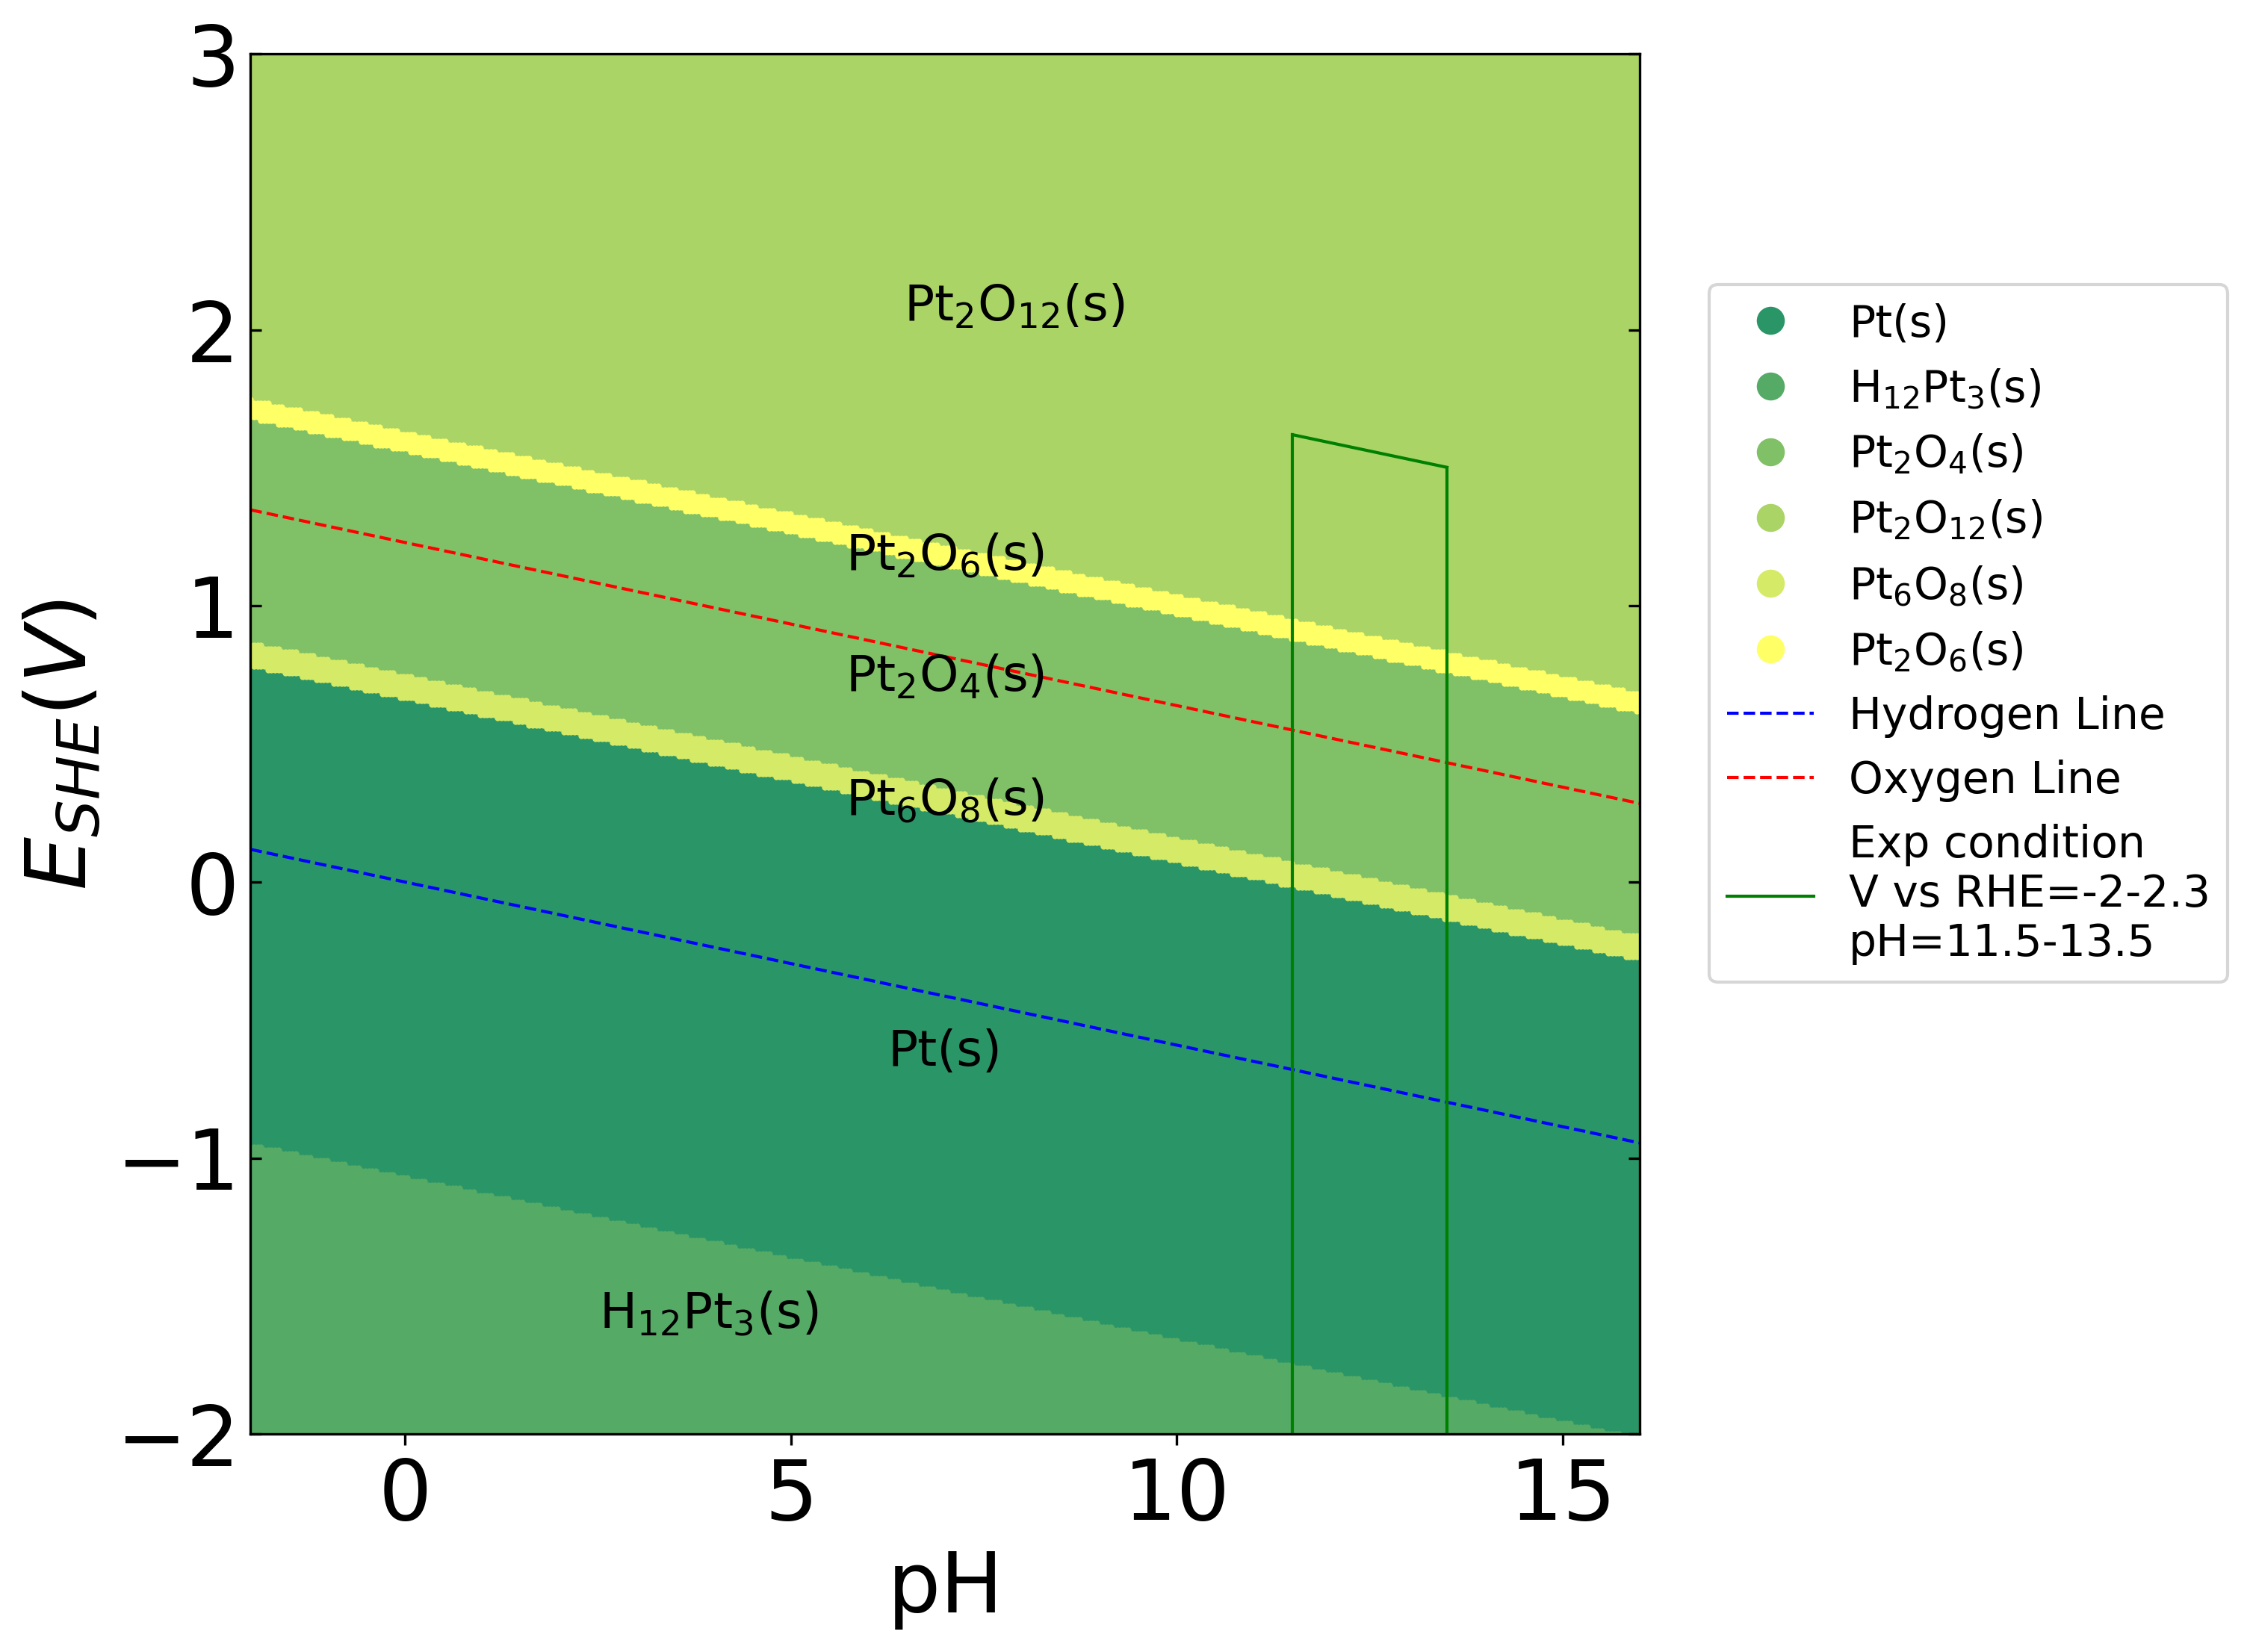
\includegraphics[width=\textwidth]{Figures/pourbaix_diagrams/Pt-NH3-H2O_activity=1e-04_[NH3]=0.02M_[Gly]=0.005M_[CN]=0.png}
%         \par\medskip
%     \end{subfigure}
%     \begin{subfigure}[b]{0.3\textwidth}
%         \subcaption{}\label{fig:Pt_Pourbaix_NH3_Gly_CN}
%         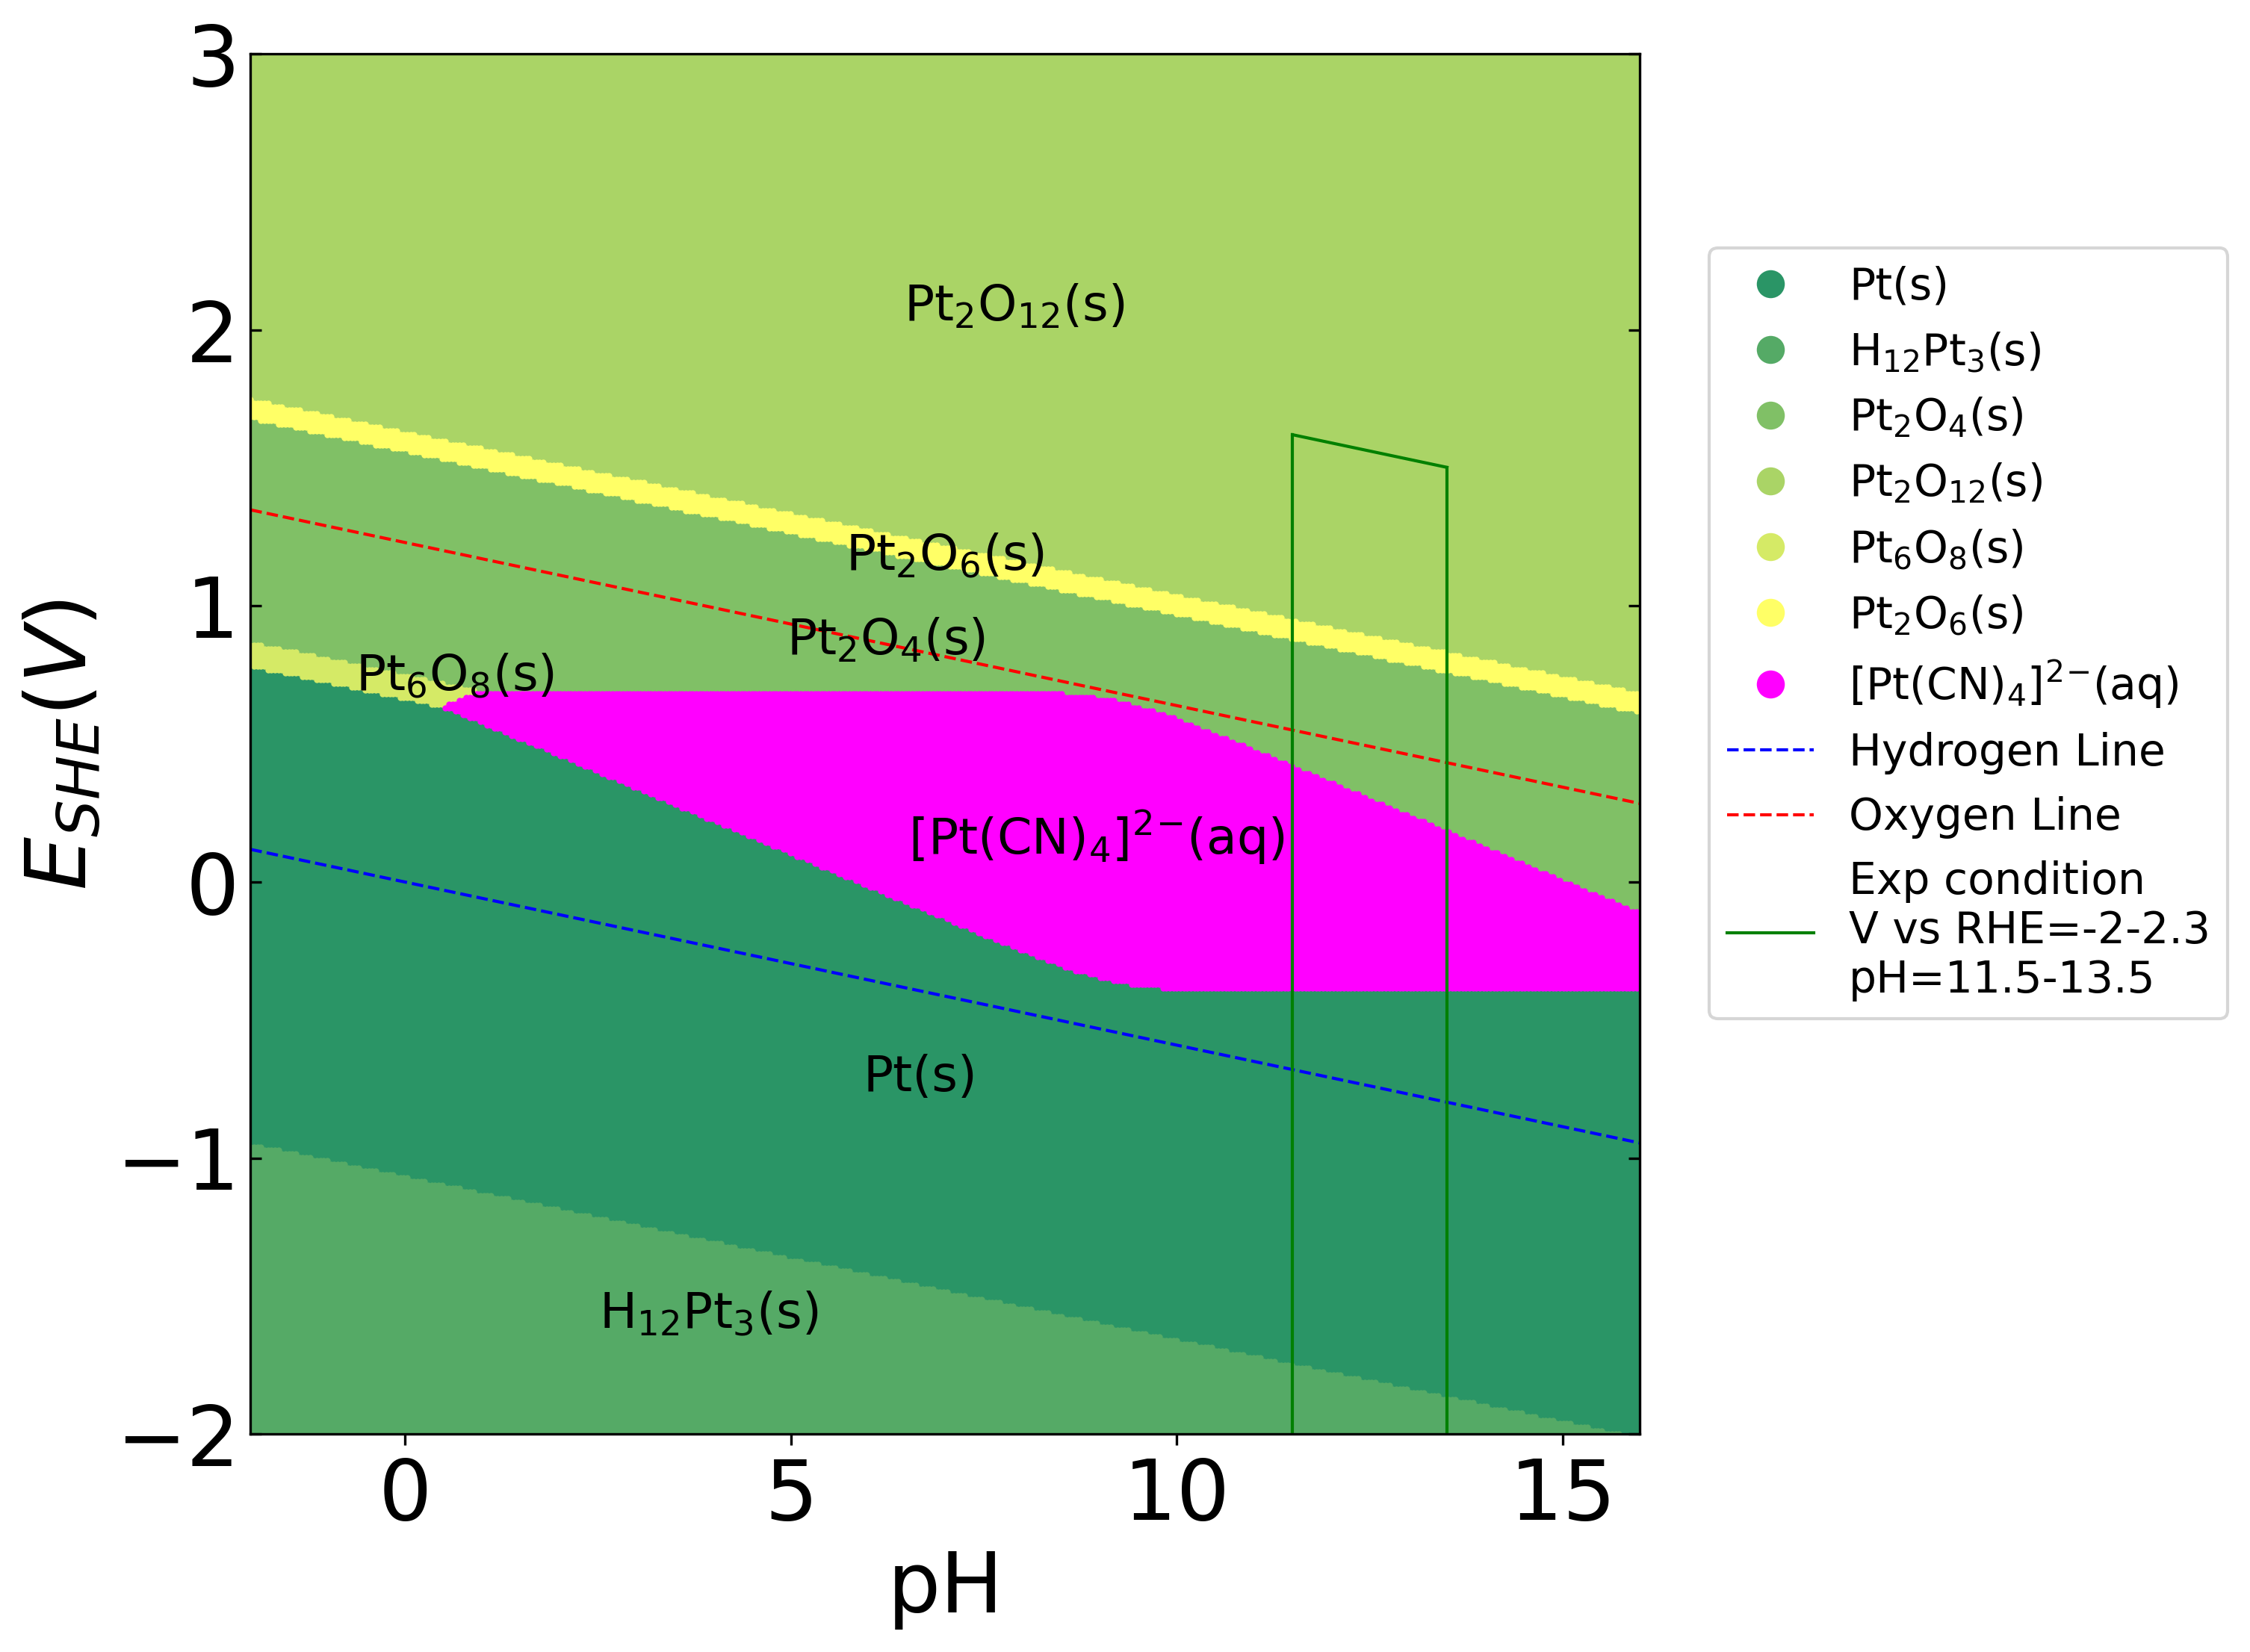
\includegraphics[width=\textwidth]{Figures/pourbaix_diagrams/Pt-NH3-H2O_activity=1e-04_[NH3]=0.02M_[Gly]=0.005M_[CN]=0.0001.png}
%         \par\medskip   
%     \end{subfigure}

%     \caption{Pt Pourbaix diagrams, with $\text{ion activity}=\num{1e-4}$, (a)$[\ce{NH3}]_{initial}= 0.02$M, $[\text{Gly}]_{initial}=0.005$M, (b)$[\ce{NH3}]_{initial}= 0.02$M, $[\text{Gly}]_{initial}=0.005$M, (c)$[\ce{NH3}]_{initial}= 0.02$M, $[\text{Gly}]_{initial}=0.005$M,  $[\ce{CN-}]_{initial}=\num{1e-4}$M. Green box indicates experimental condition at applied potential vs RHE = -2 to 2V, pH = 11.5 to 13.5.}
%     \label{fig:Pt_Pourbaix}
% \end{figure}

%%%%%%%%%%%%%%%%%%%%%%%%%%%%%%%%% Pt and Ti %%%%%%%%%%%%%%%%%%%%%%%%%%%%%%%%%
\begin{figure}[htbp]
    \centering
    \begin{subfigure}[b]{0.45\textwidth}
        \subcaption{}\label{fig:Ti_Pourbaix_NH3_Gly_CN}
        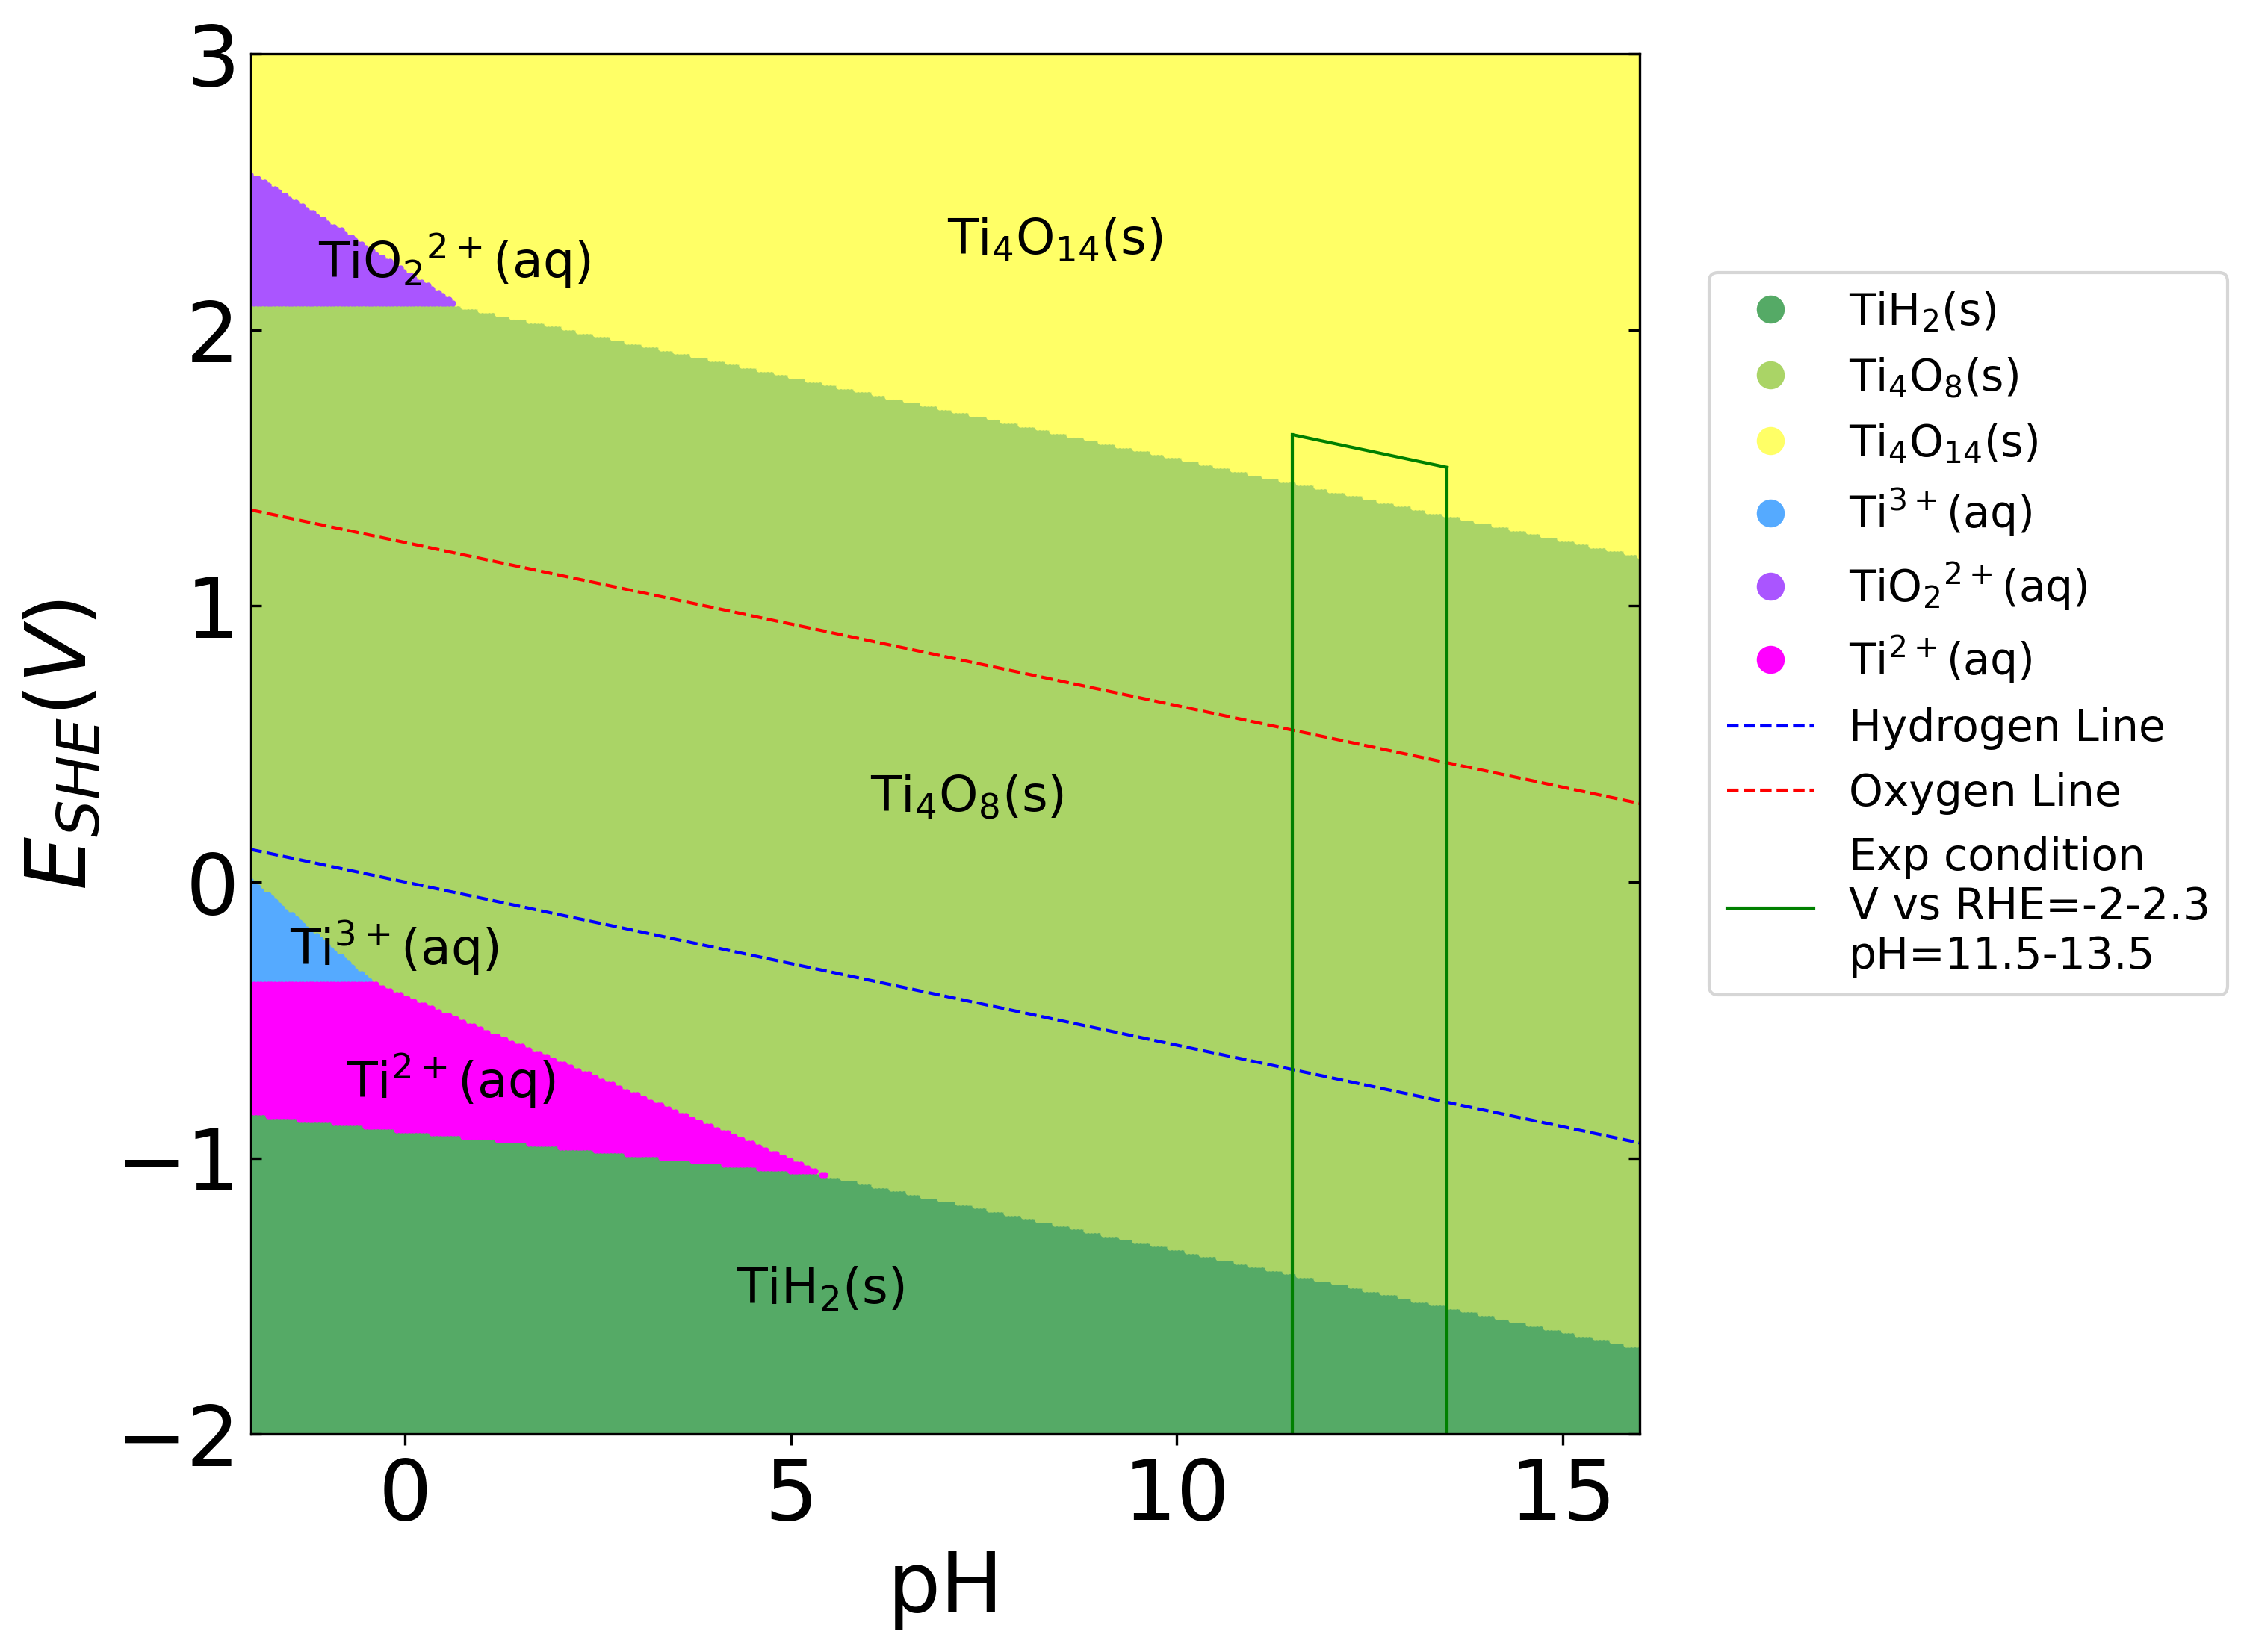
\includegraphics[width=\textwidth]{Figures/pourbaix_diagrams/Ti-NH3-H2O_activity=1e-04_[NH3]=0.02M_[Gly]=0.005M_[CN]=0.0001.png}
        \par\medskip
    \end{subfigure}
    \begin{subfigure}[b]{0.45\textwidth}
        \subcaption{}\label{fig:Pt_Pourbaix_NH3_Gly_CN}
        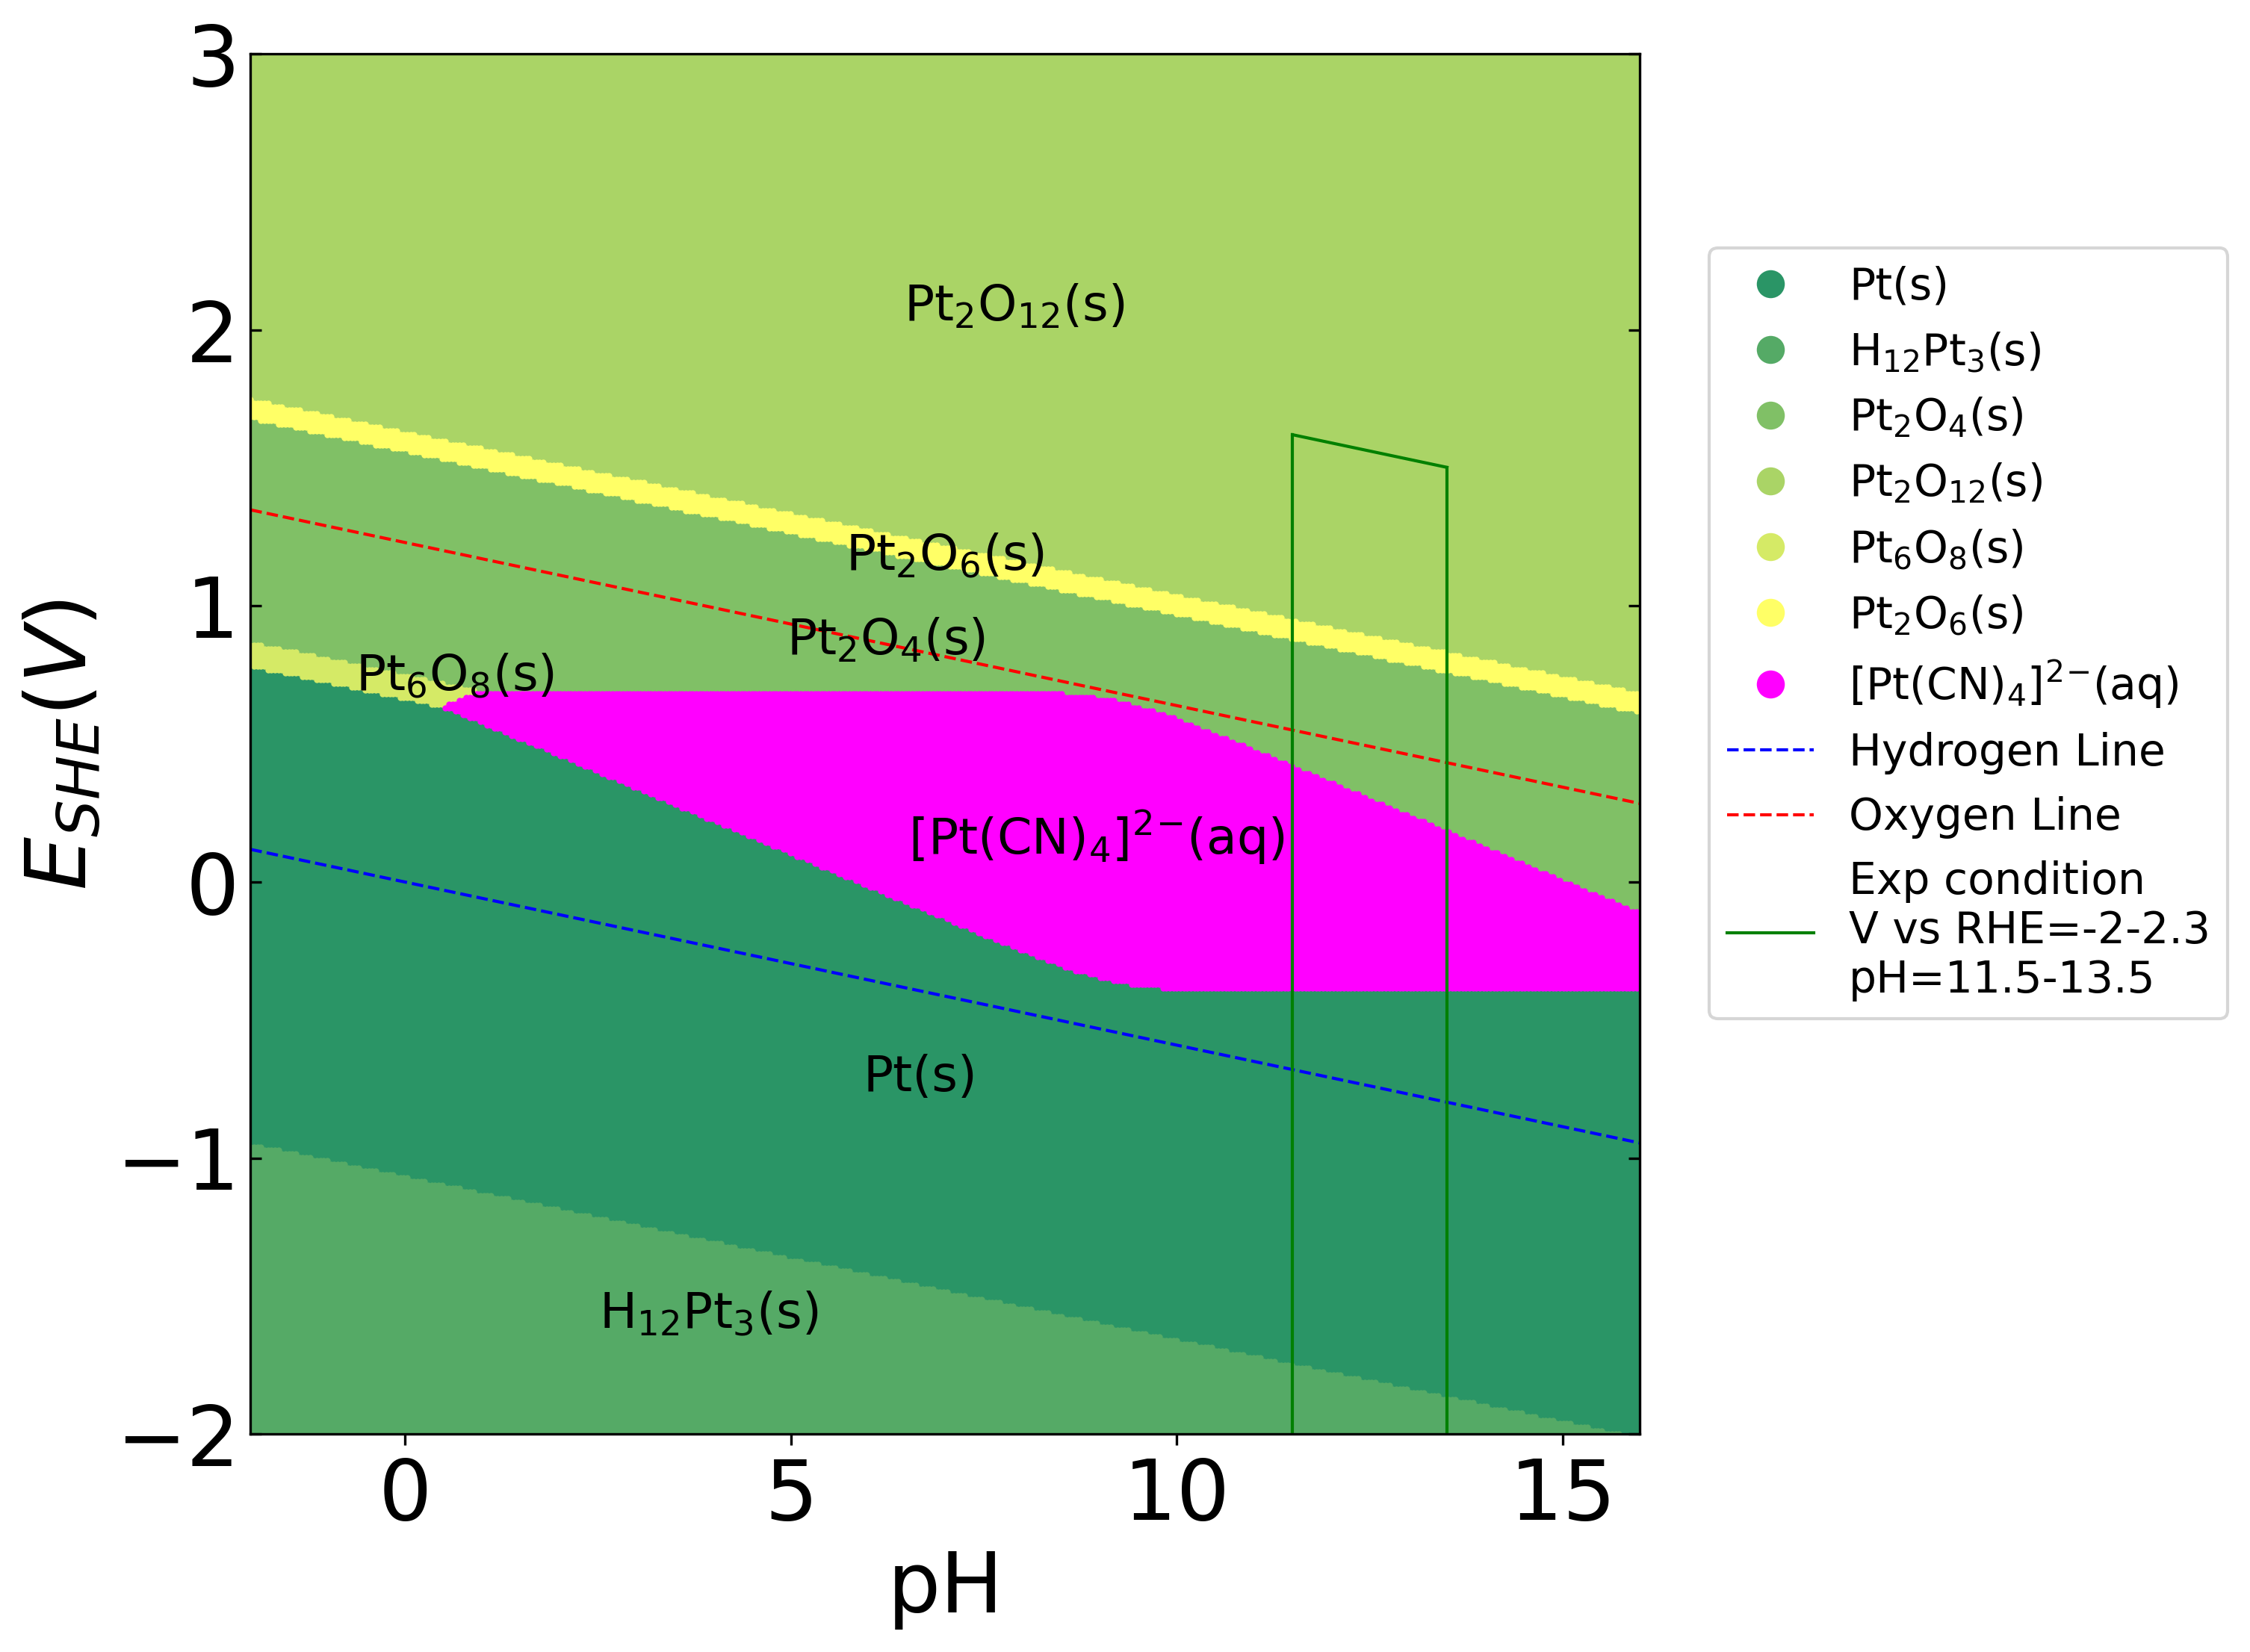
\includegraphics[width=\textwidth]{Figures/pourbaix_diagrams/Pt-NH3-H2O_activity=1e-04_[NH3]=0.02M_[Gly]=0.005M_[CN]=0.0001.png}
        \par\medskip   
    \end{subfigure}
    \caption{Pourbaix diagrams of (a) Ti, (b) Pt. $\text{Ion activity}=\num{1e-4}$, $[\ce{NH3}]_{initial}= 0.02$M, $[\text{Gly}]_{initial}=0.005$M,  $[\ce{CN-}]_{initial}=\num{1e-4}$M. Green box indicates experimental condition at applied potential vs RHE = -2 to 2V, pH = 11.5 to 13.5.}
    \label{fig:Ti_Pt_Pourbaix}
\end{figure}

% %%%%%%%%%%%%%%%%%%%%%%%%%%%%%%%%% Ti %%%%%%%%%%%%%%%%%%%%%%%%%%%%%%%%%
% \begin{figure}
%     \centering
%     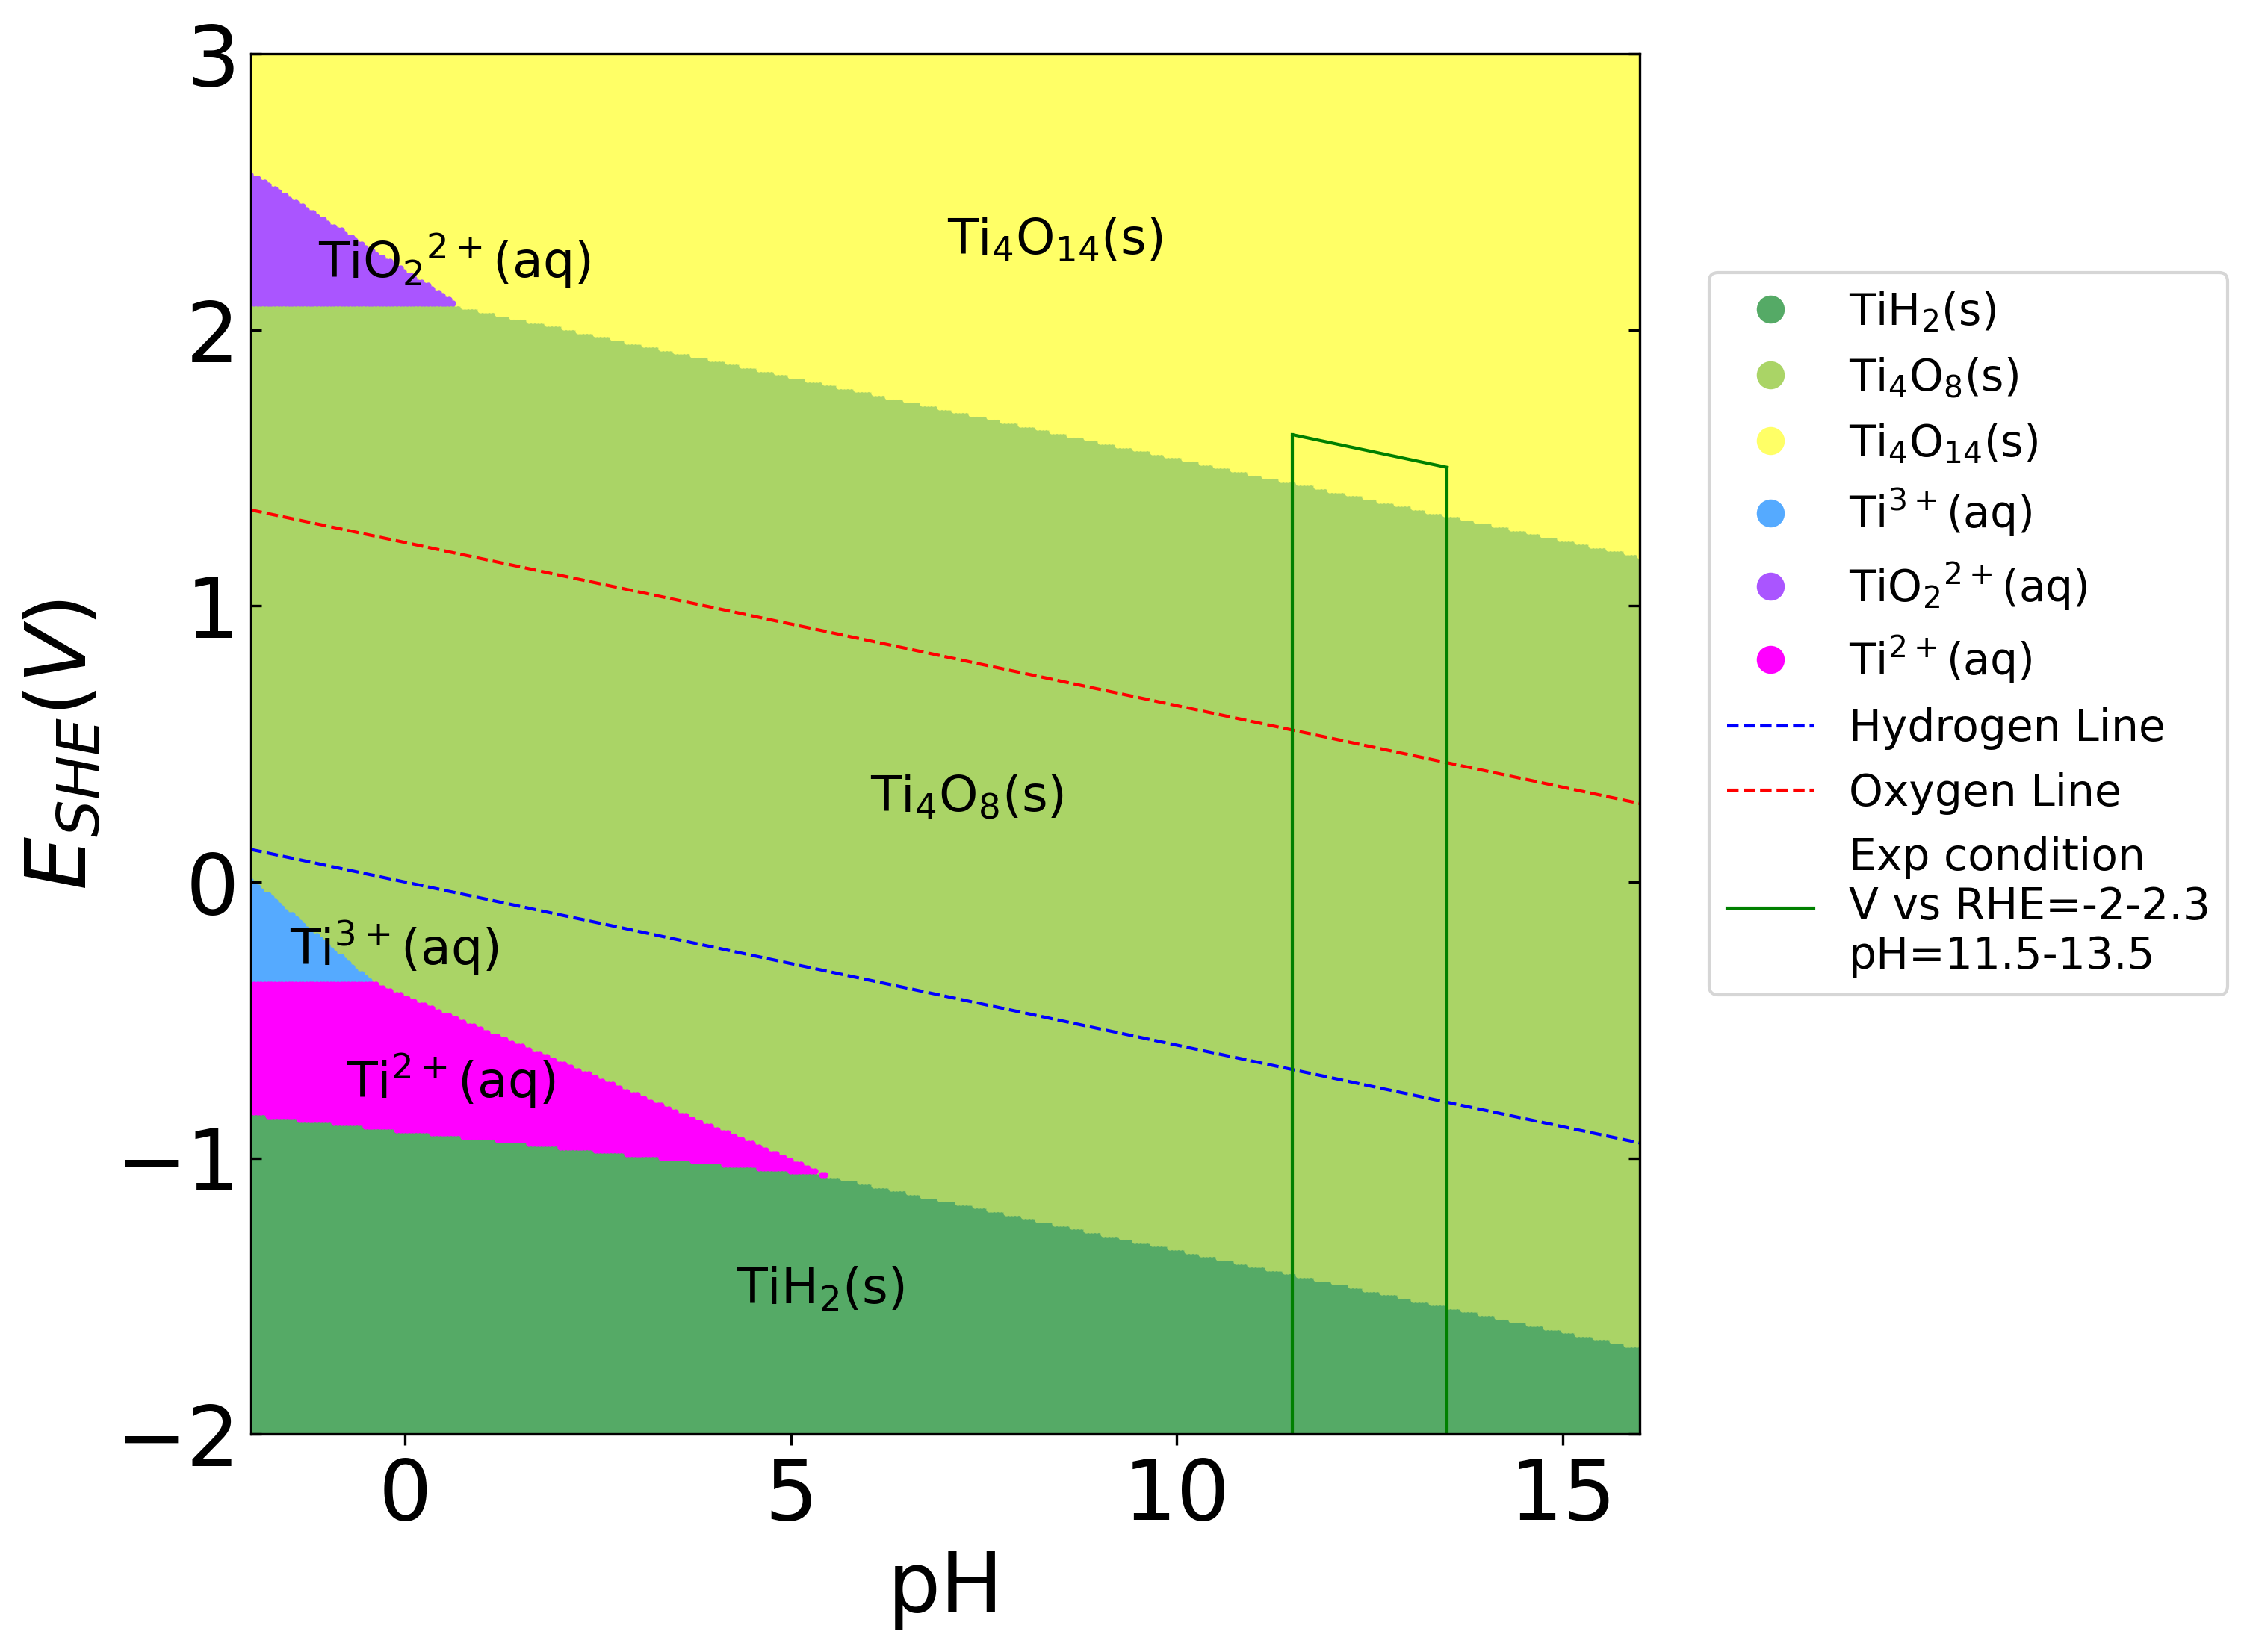
\includegraphics[width=0.6\linewidth]{Figures/pourbaix_diagrams/Ti-NH3-H2O_activity=1e-04_[NH3]=0.02M_[Gly]=0.005M_[CN]=0.0001.png}
%     \caption{Ti Pourbaix diagram, with with $\text{ion activity}=\num{1e-4}$,$[\ce{NH3}]_{initial}= 0.02$M, $[\text{Gly}]_{initial}=0.005$M,  $[\ce{CN-}]_{initial}=\num{1e-4}$M. Green box indicates experimental condition at applied potential vs RHE = -2 to 2V, pH = 11.5 to 13.5.}
%     \label{fig:Ti_Pourbaix}
% \end{figure}
%%%%%%%%%%%%%%%%%%%%%%%%%%%%%%%%% NH3 and Gly only %%%%%%%%%%%%%%%%%%%%%%%%%%%%%%%%%
% \begin{figure}[htbp]
%     \centering
%     % Subfigure (a)
%     \begin{subfigure}[b]{0.3\textwidth}
%         \subcaption{}\label{fig:Ni_Pourbaix_NH3_Gly}
%         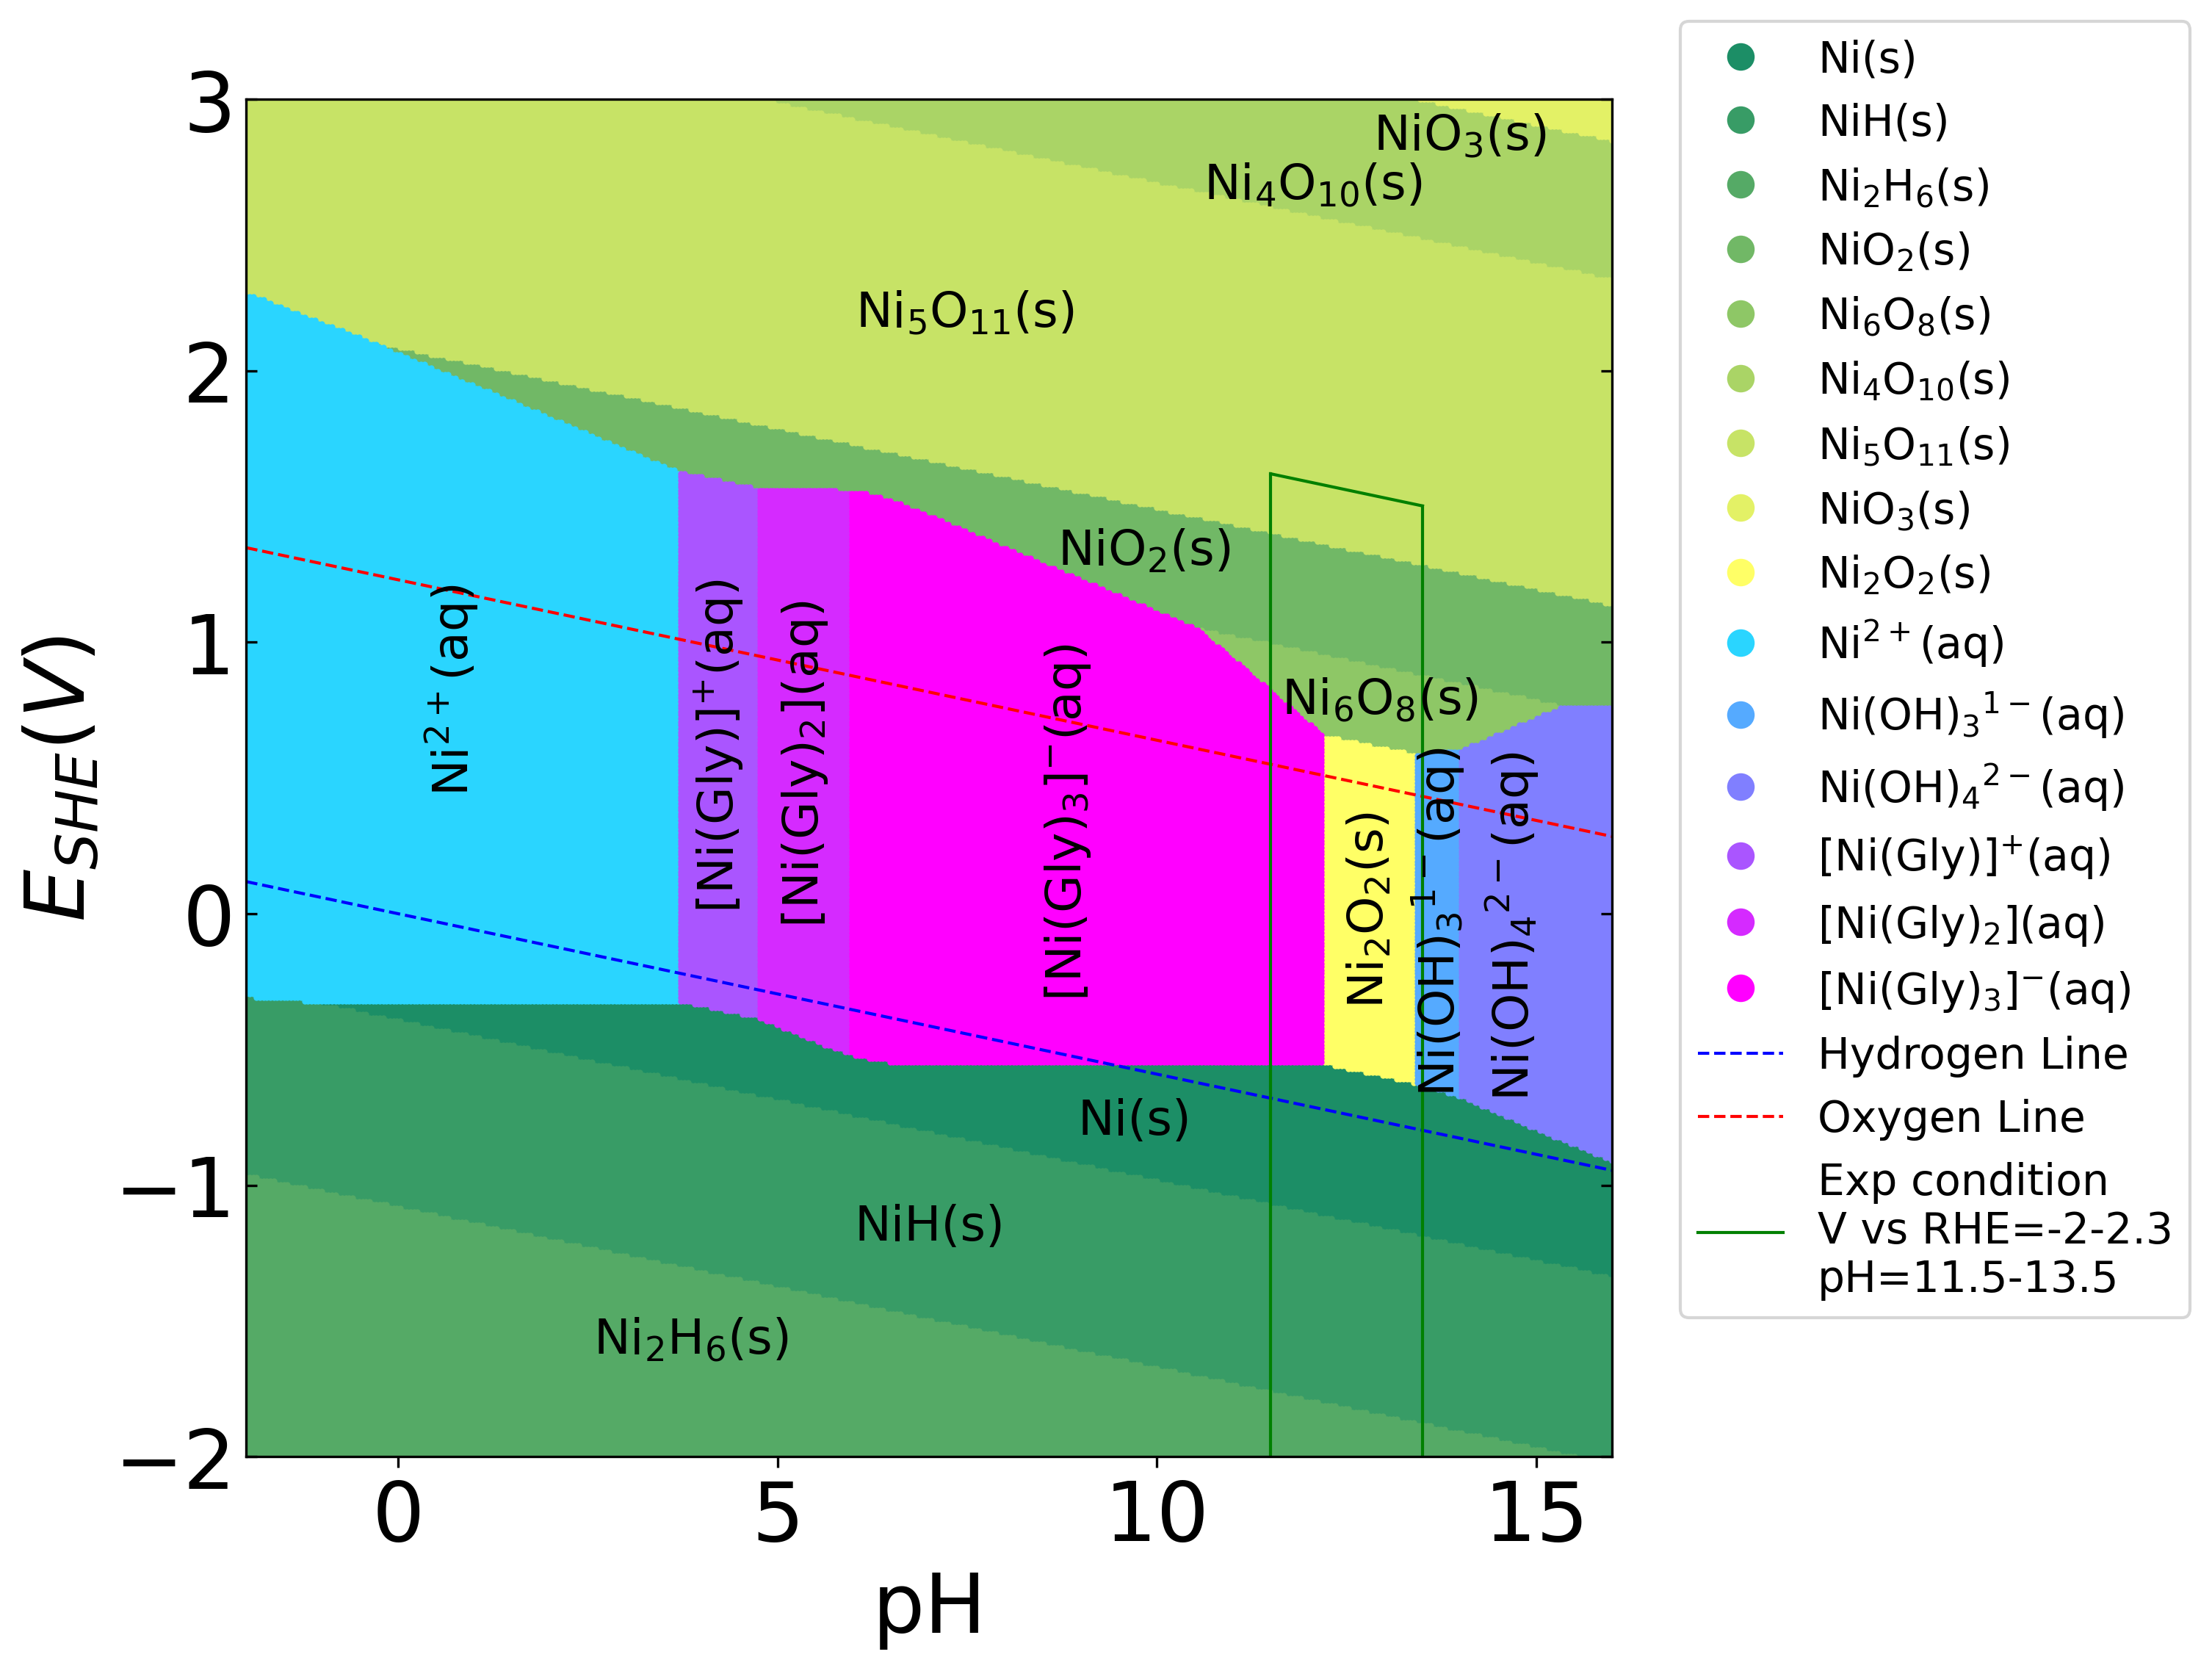
\includegraphics[width=\textwidth]{Figures/pourbaix_diagrams/Ni-NH3-H2O_activity=1e-04_[NH3]=0.02M_[Gly]=0.005M_[CN]=0.png}
%         \par\medskip
%     \end{subfigure}
%     % Subfigure (b)
%     \begin{subfigure}[b]{0.3\textwidth}
%         \subcaption{}\label{fig:Au_Pourbaix_NH3_Gly}
%         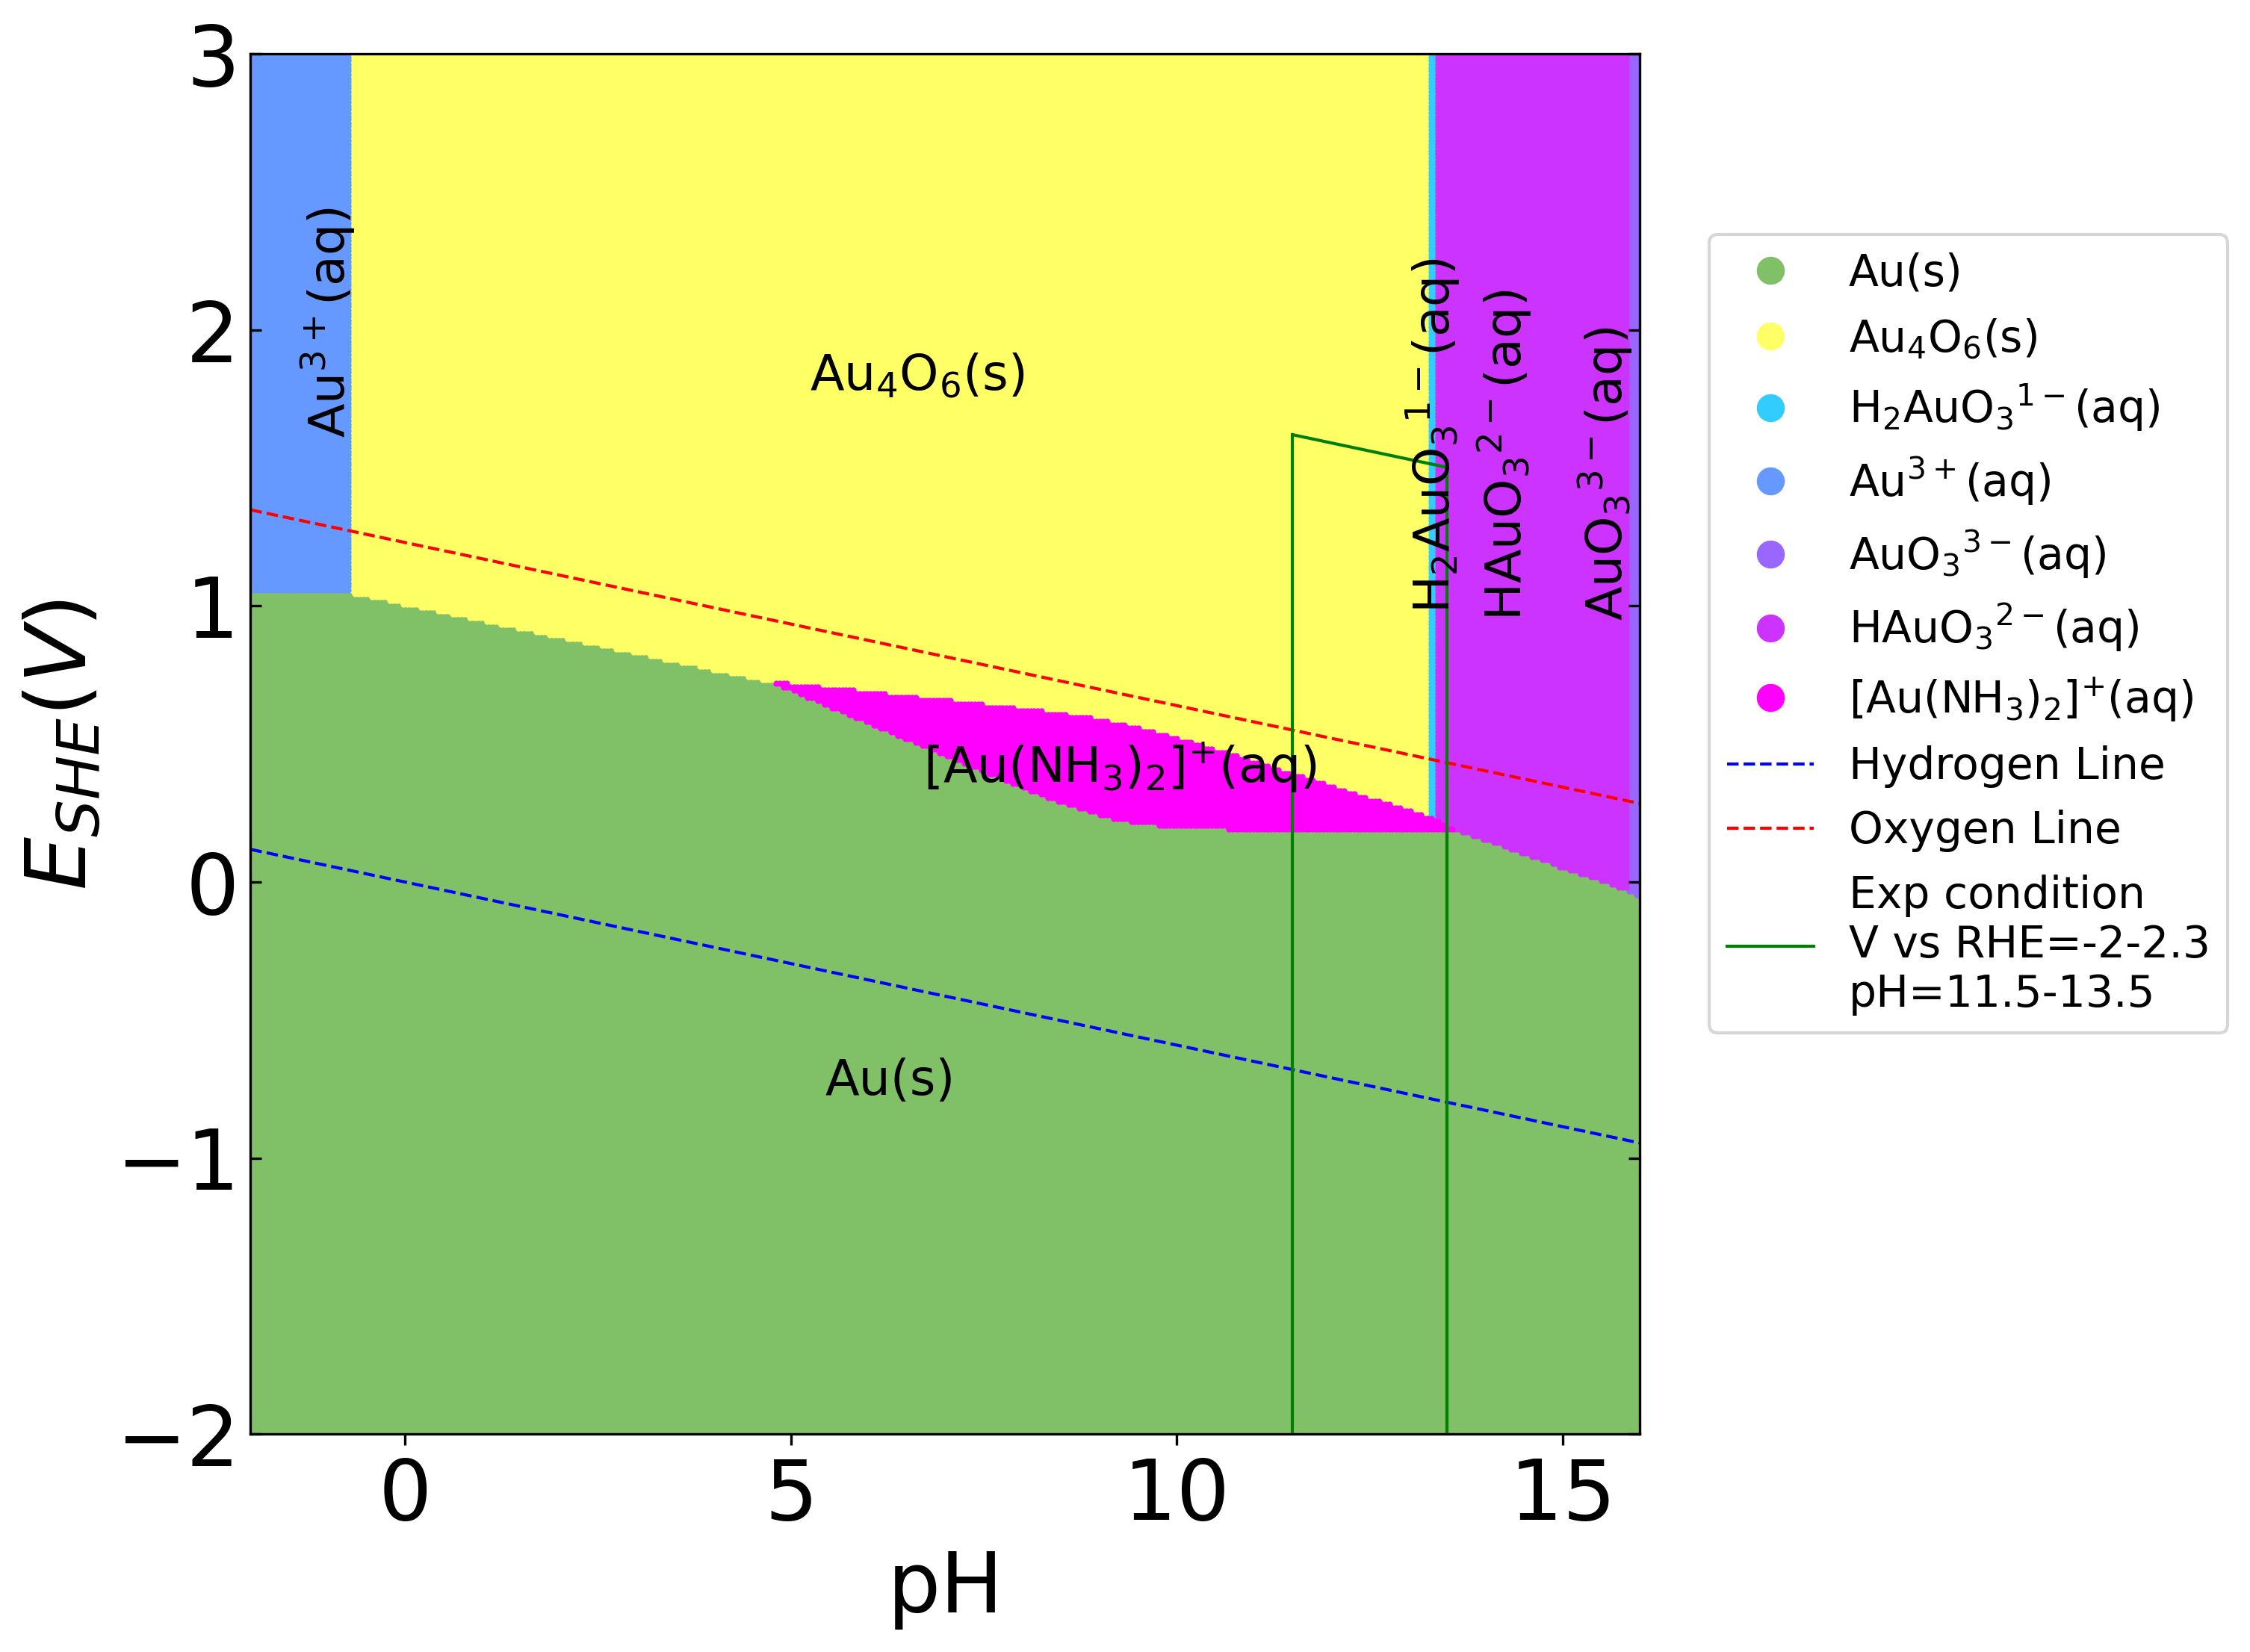
\includegraphics[width=\textwidth]{Figures/pourbaix_diagrams/Au-NH3-H2O_activity=1e-04_[NH3]=0.02M_[Gly]=0.005M_[CN]=0.png}
%         \par\medskip
%     \end{subfigure}
%     % Subfigure (c)
%     \begin{subfigure}[b]{0.3\textwidth}
%         \subcaption{}\label{fig:Cu_Pourbaix_NH3_Gly}
%         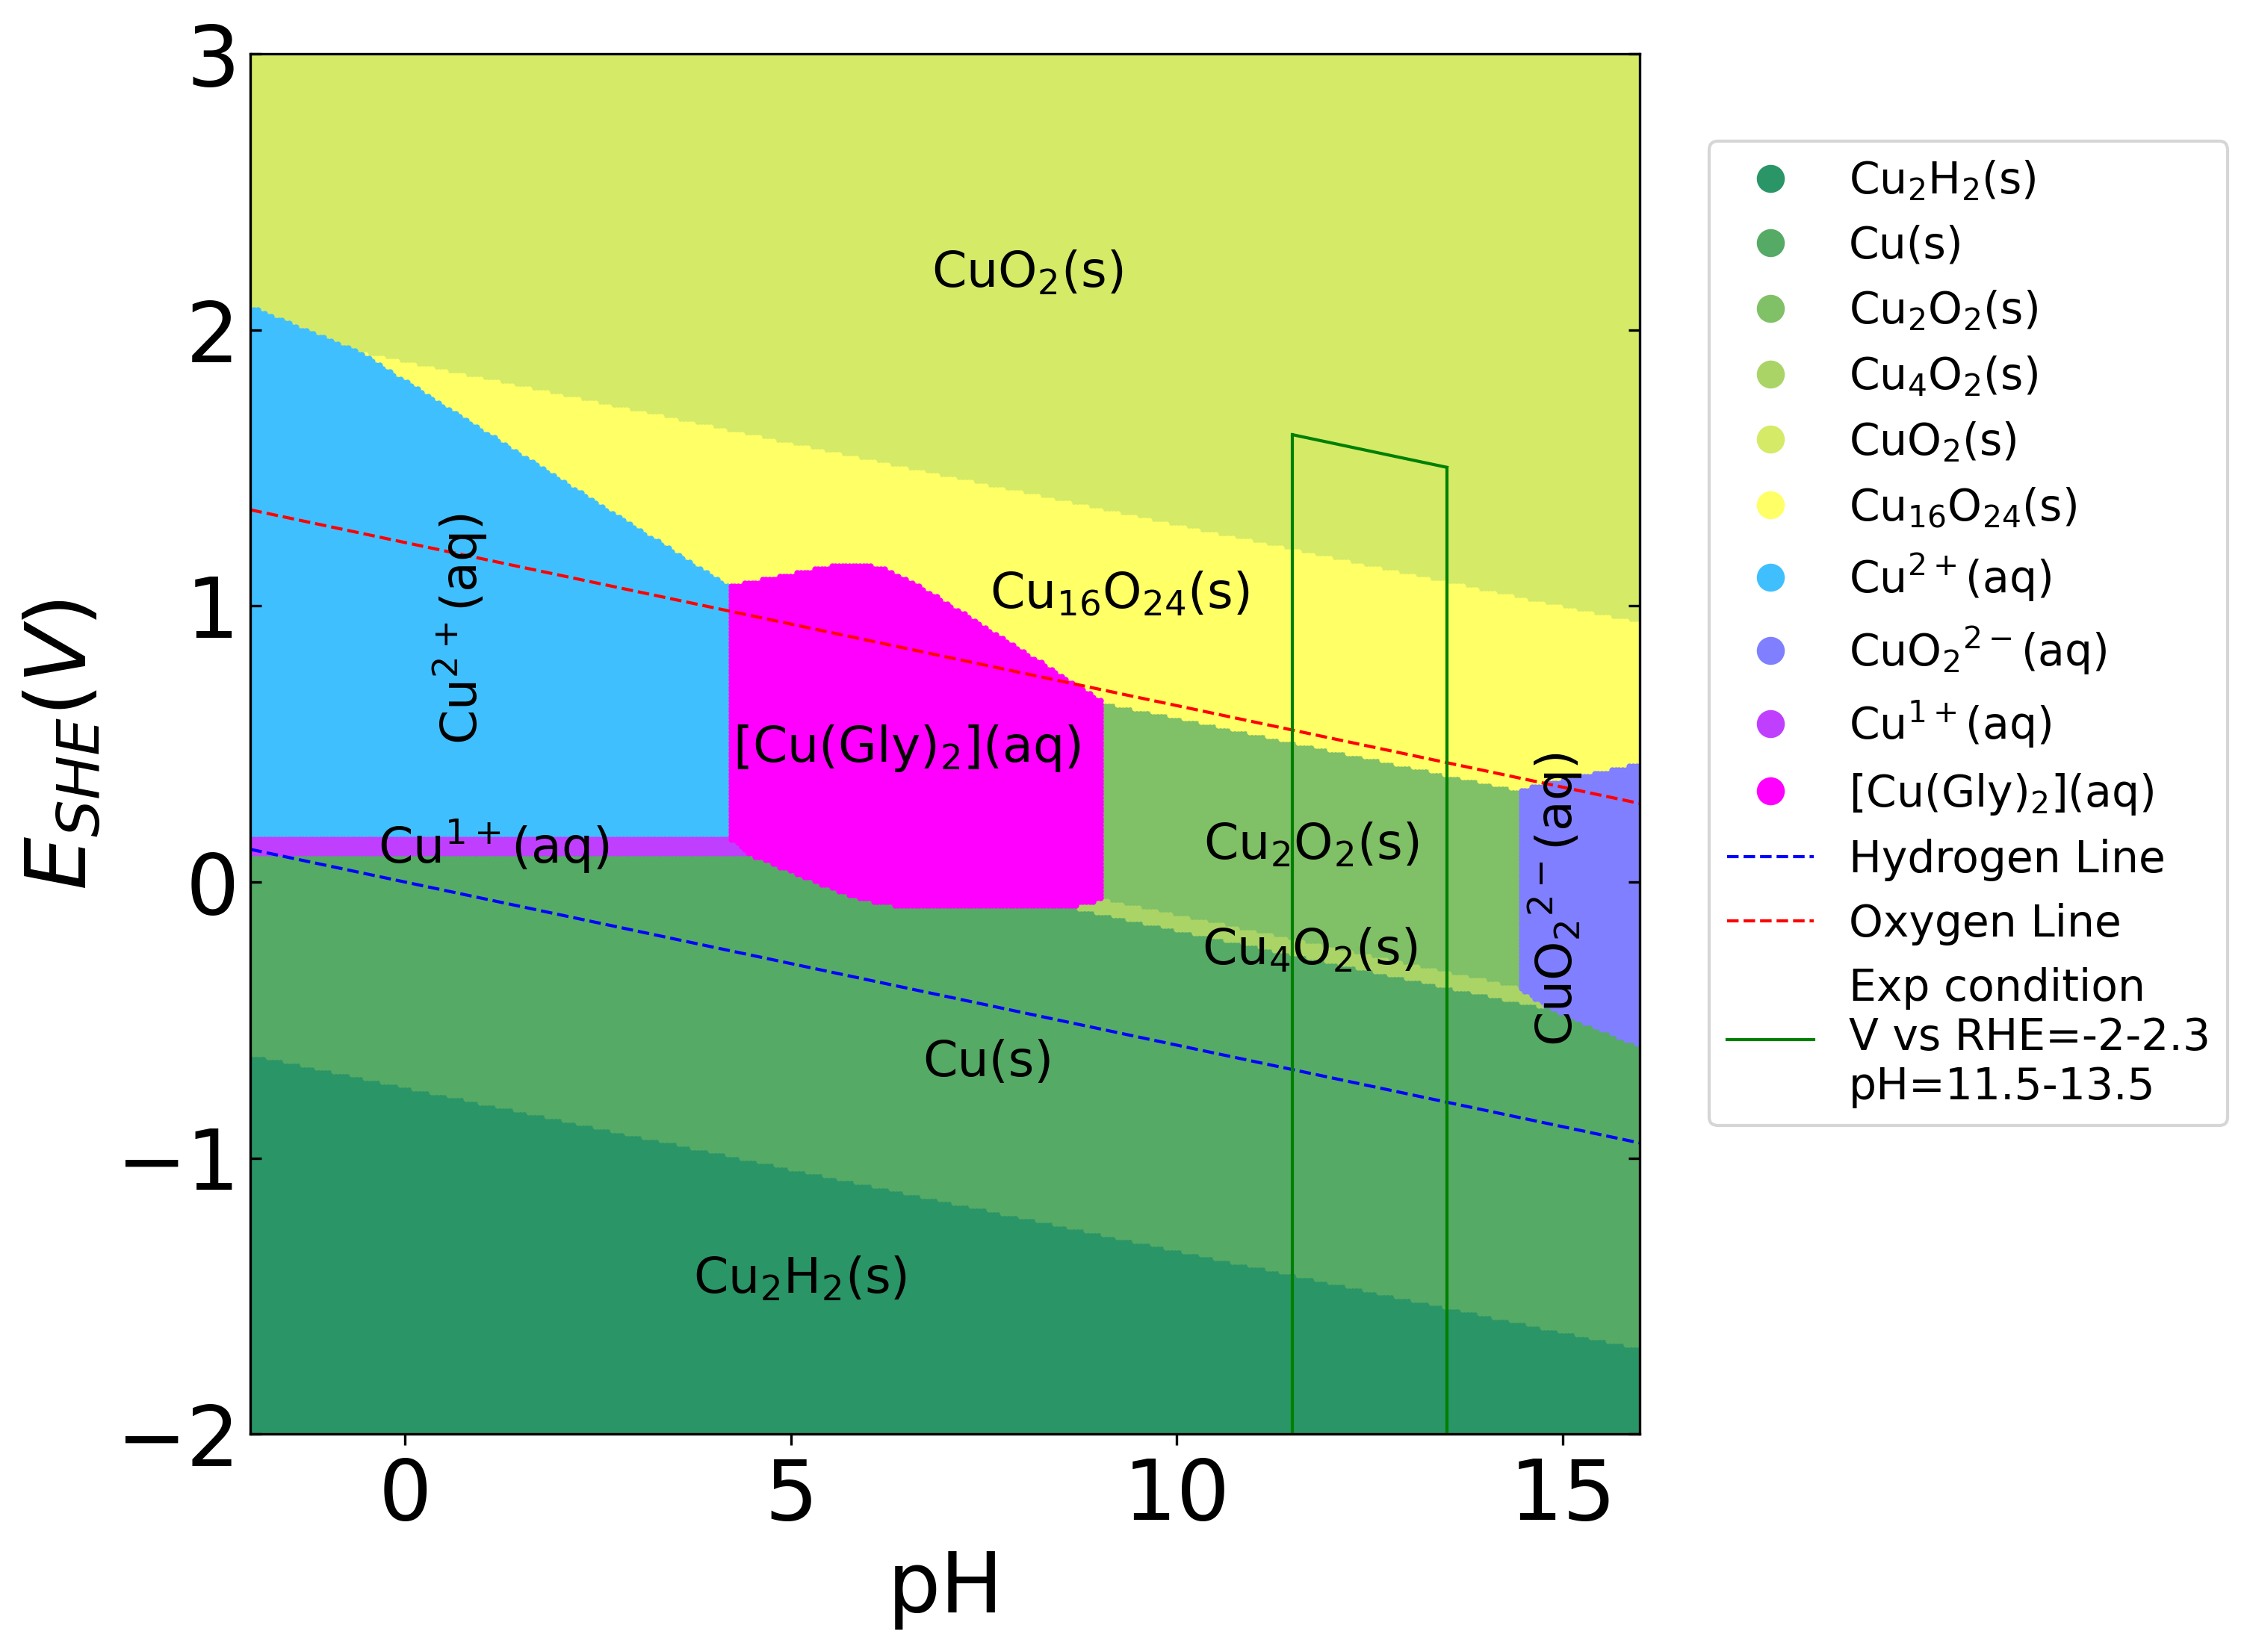
\includegraphics[width=\textwidth]{Figures/pourbaix_diagrams/Cu-NH3-H2O_activity=1e-04_[NH3]=0.02M_[Gly]=0.005M_[CN]=0.png}
%         \par\medskip   
%     \end{subfigure}
%     % Subfigure (d)
%     \begin{subfigure}[b]{0.3\textwidth}
%         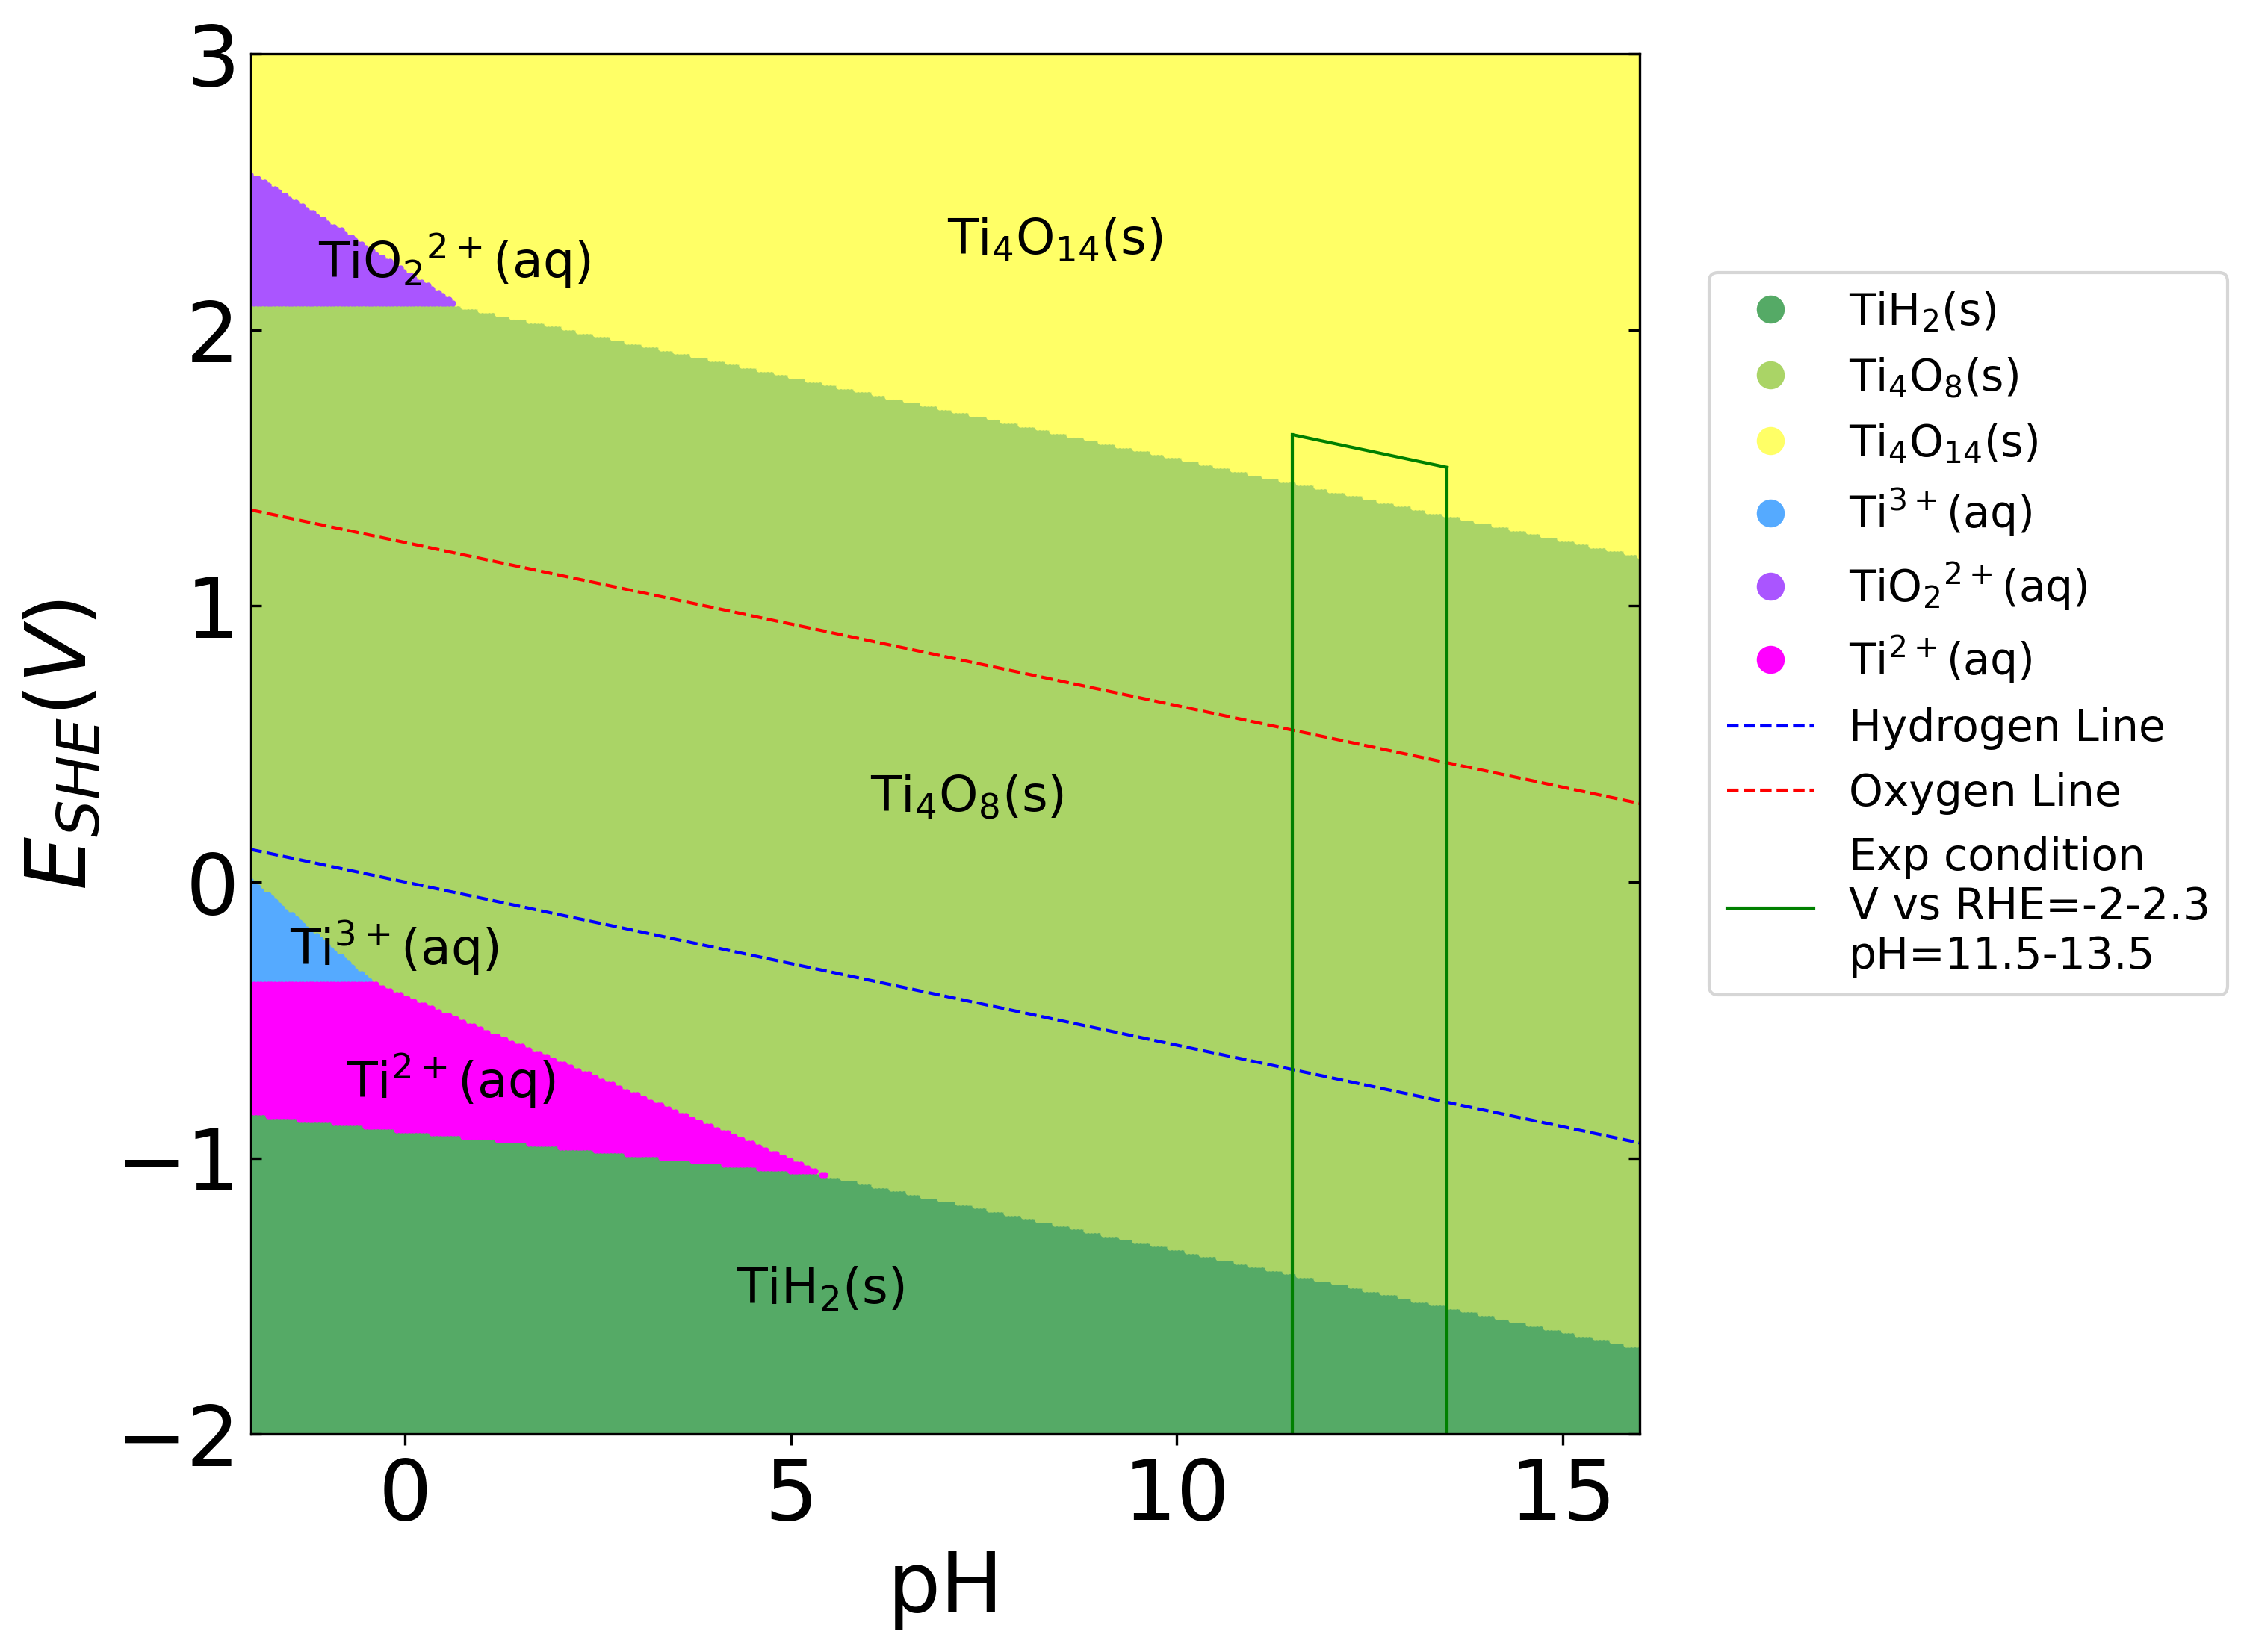
\includegraphics[width=\textwidth]{Figures/pourbaix_diagrams/Ti-NH3-H2O_activity=1e-04_[NH3]=0.02M_[Gly]=0.005M_[CN]=0.png}
%         \subcaption{}\label{fig:Ti_Pourbaix_NH3_Gly}
%     \end{subfigure}
%     % Subfigure (e)
%     \begin{subfigure}[b]{0.3\textwidth}
%         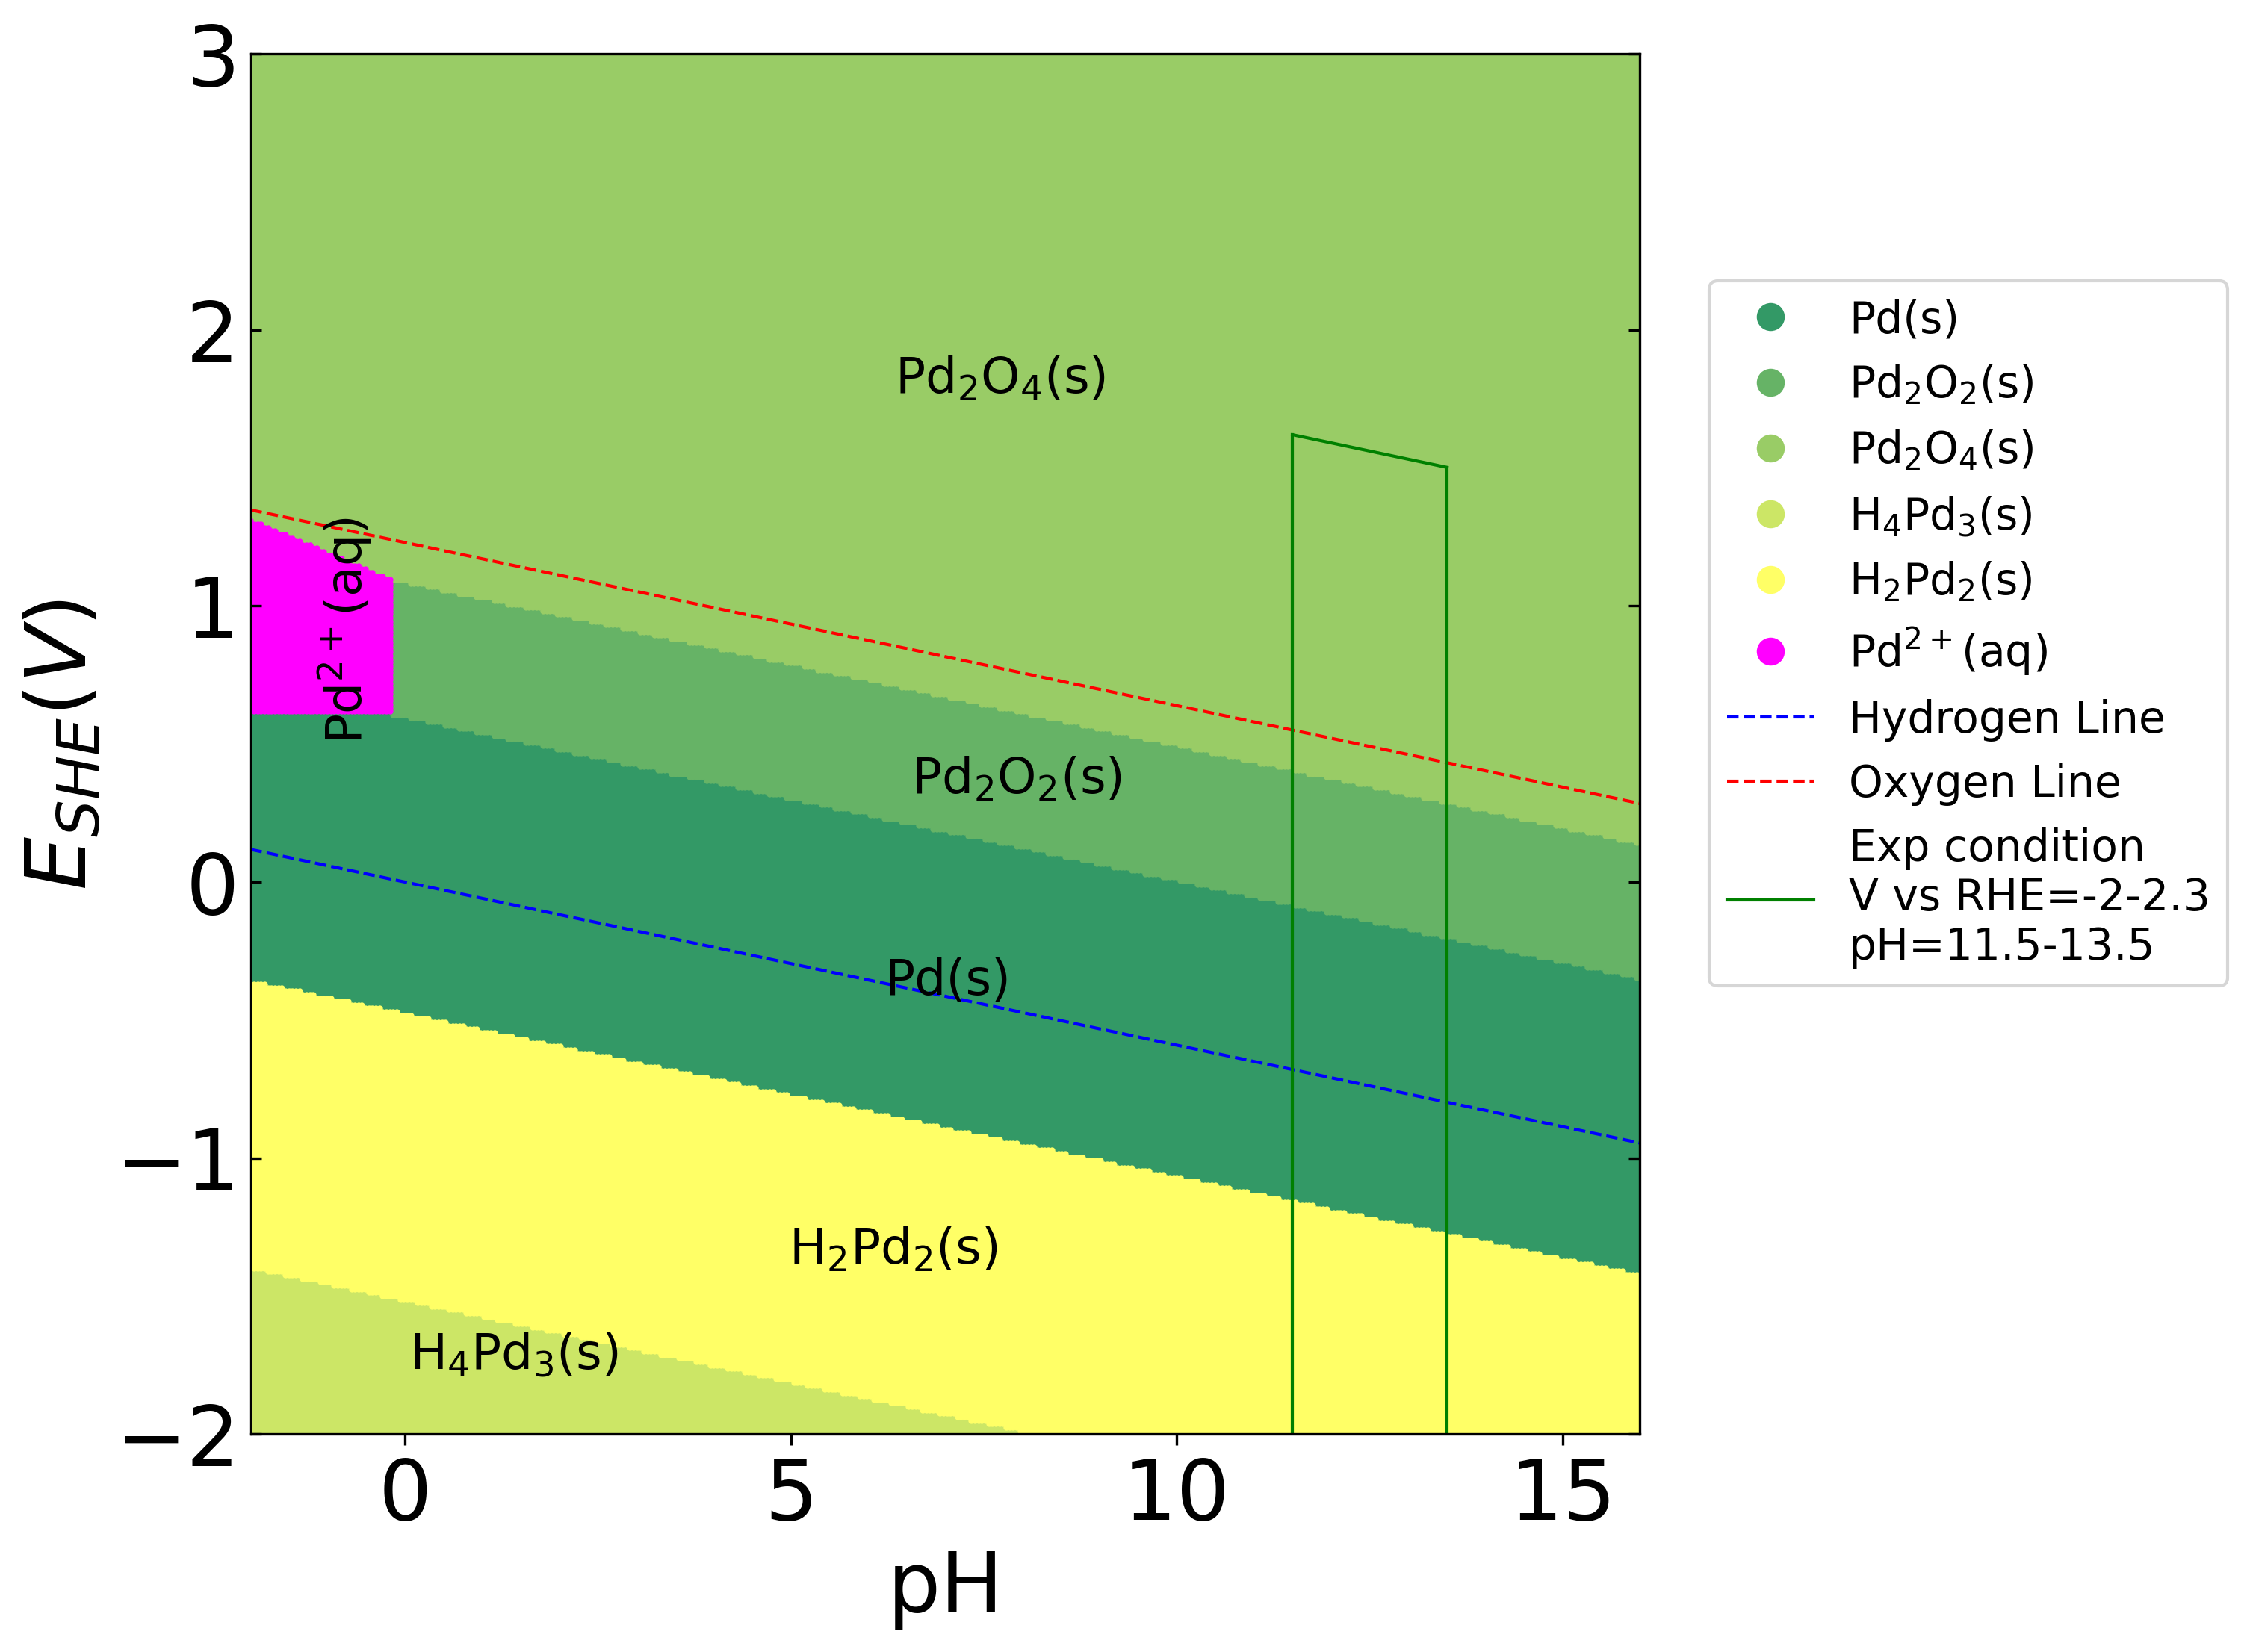
\includegraphics[width=\textwidth]{Figures/pourbaix_diagrams/Pd-NH3-H2O_activity=1e-04_[NH3]=0.02M_[Gly]=0.005M_[CN]=0.png}
%         \subcaption{}\label{fig:Pd_Pourbaix_NH3_Gly}
%     \end{subfigure}
%     % Subfigure (f)
%     \begin{subfigure}[b]{0.3\textwidth}
%         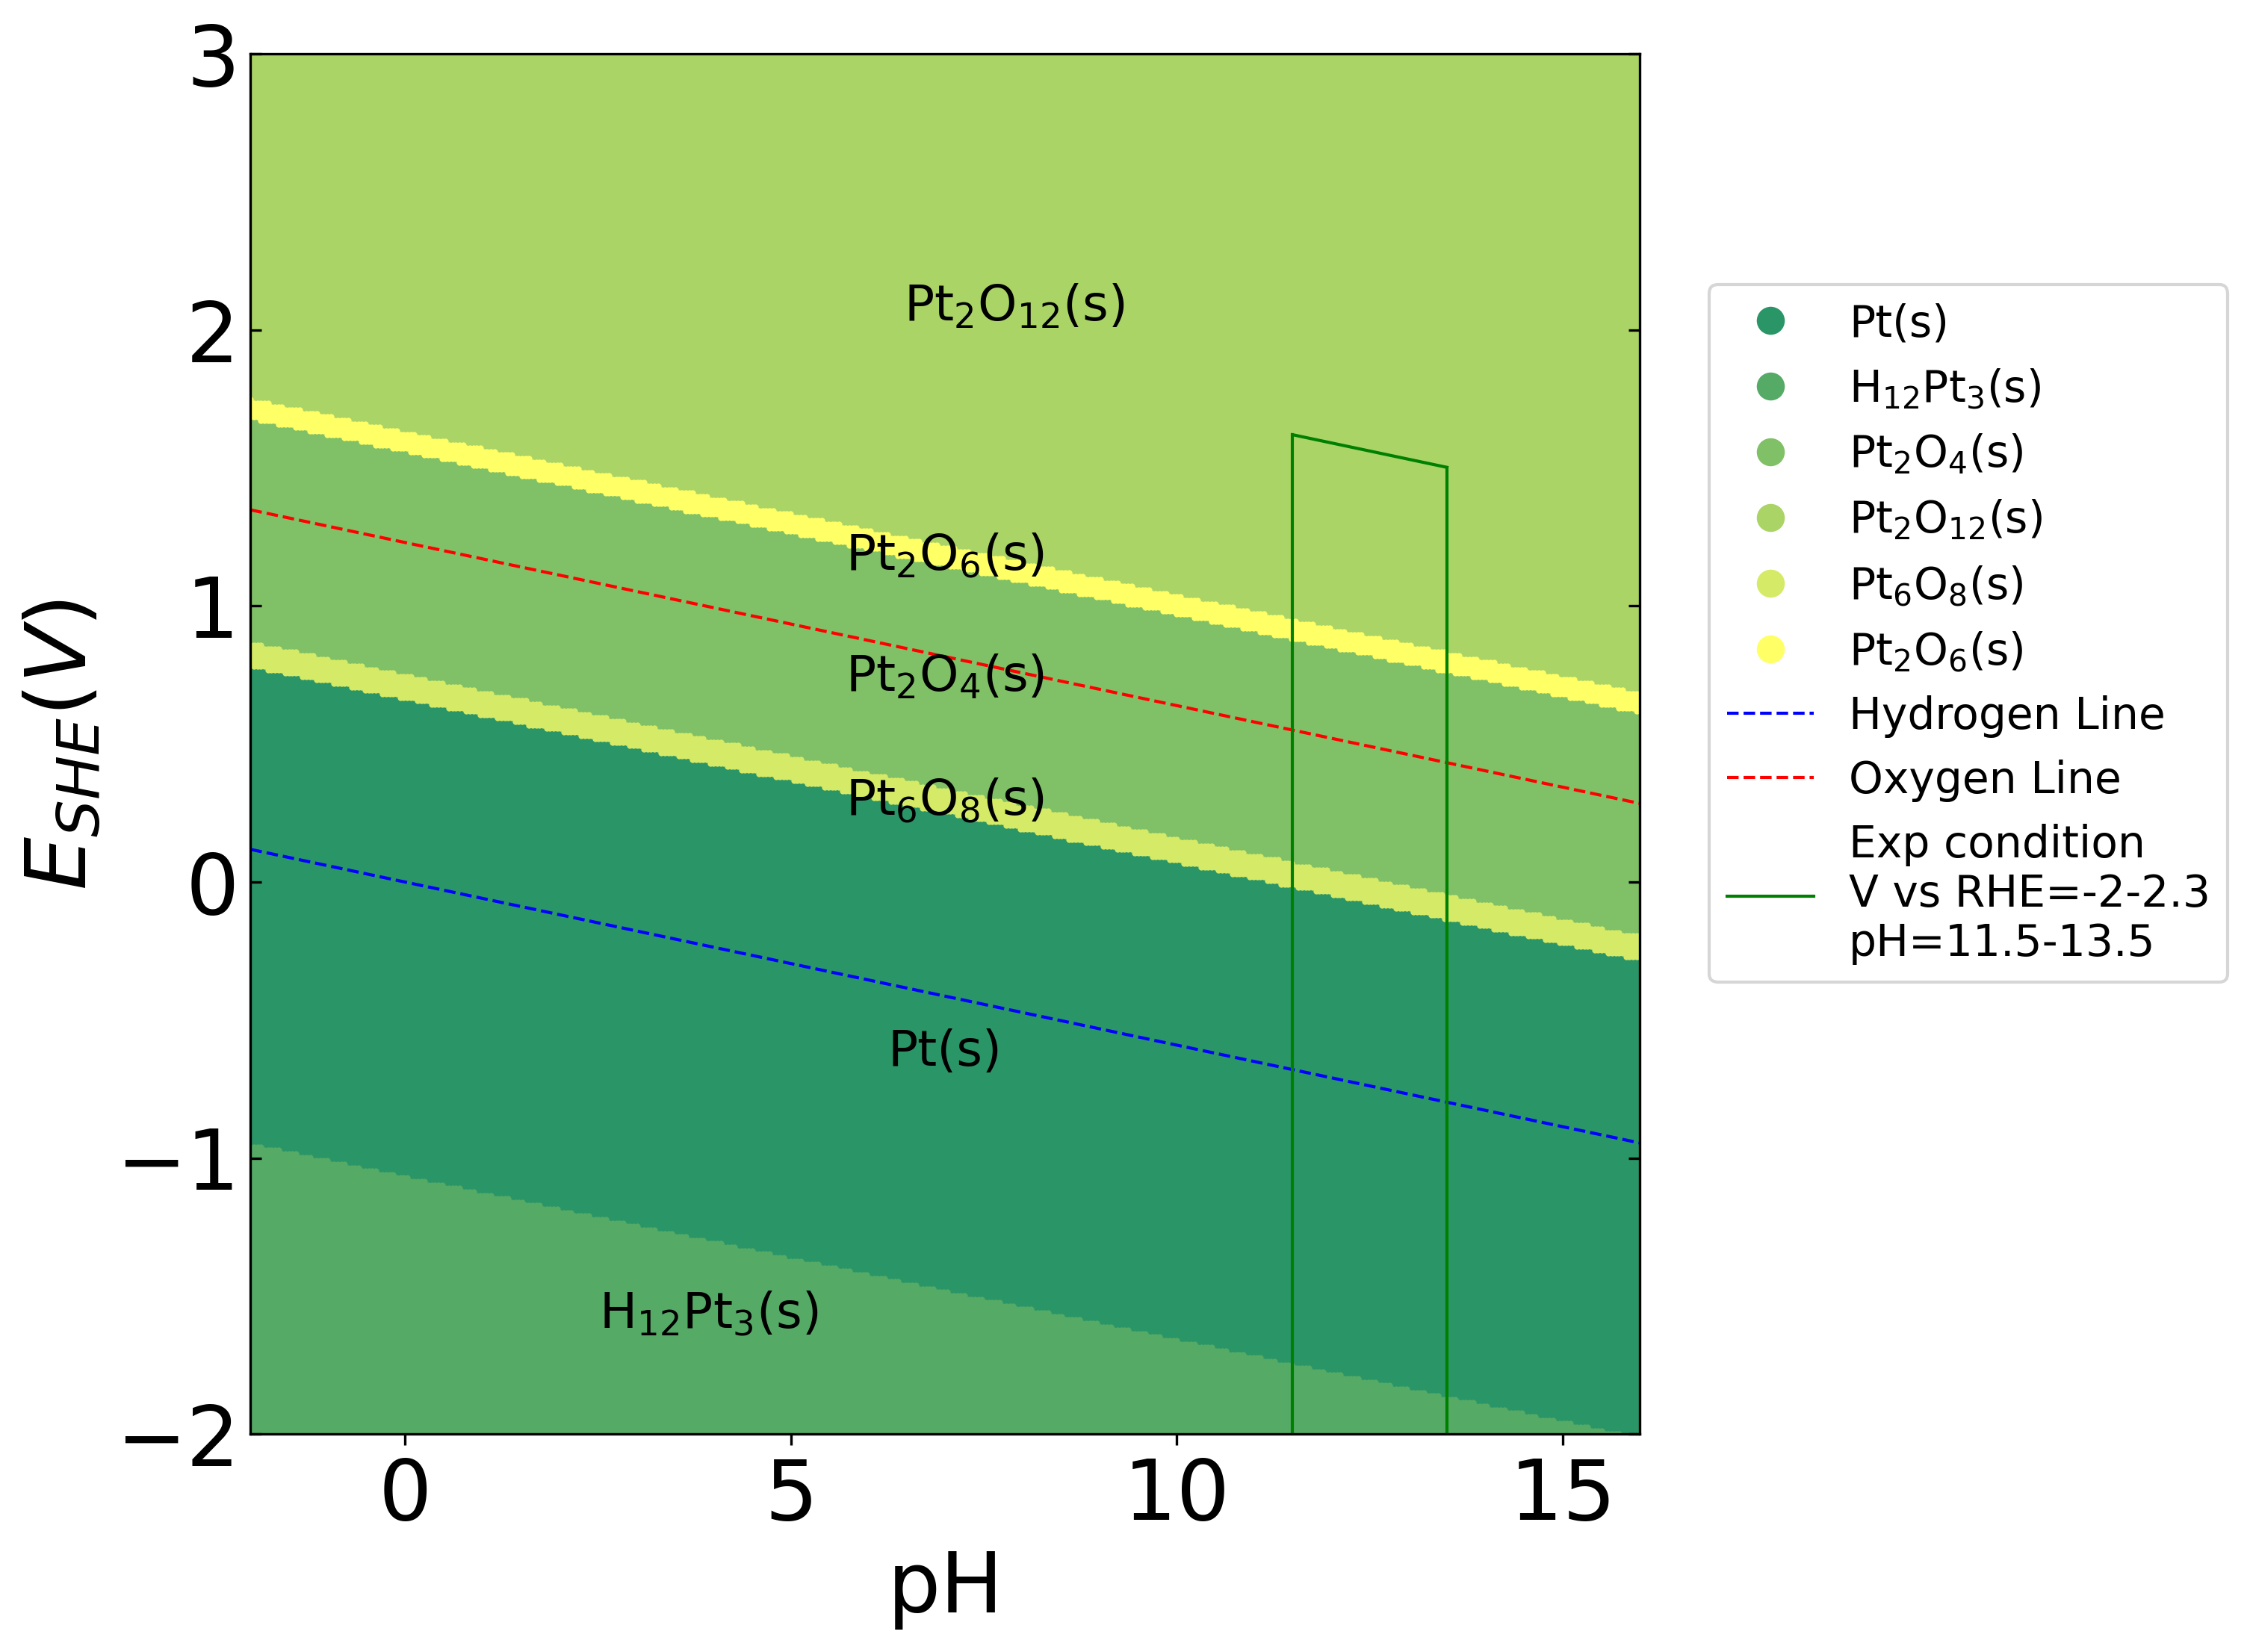
\includegraphics[width=\textwidth]{Figures/pourbaix_diagrams/Pt-NH3-H2O_activity=1e-04_[NH3]=0.02M_[Gly]=0.005M_[CN]=0.png}
%         \subcaption{}\label{fig:Pt_Pourbaix_NH3_Gly}
%     \end{subfigure}
%     \caption{Pourbaix diagrams for different metals at $[\ce{NH3}]_{initial}= 0.02$M, $[\text{Gly}]_{initial}=0.005$M. Green box indicates experimental condition at applied potential vs RHE = -2 to 2V, pH = 11.5 to 13.5.}
%     \label{fig:Pourbaix_NH3_Gly}
% \end{figure}
%%%%%%%%%%%%%%%%%%%%%%%%%%%%%%%%% H2O only %%%%%%%%%%%%%%%%%%%%%%%%%%%%%%%%%

% \begin{figure}[htbp]
%     \centering
%     % Subfigure (a)
%     \begin{subfigure}[b]{0.3\textwidth}
%         \subcaption{}\label{fig:Ni_Pourbaix_H2O}
%         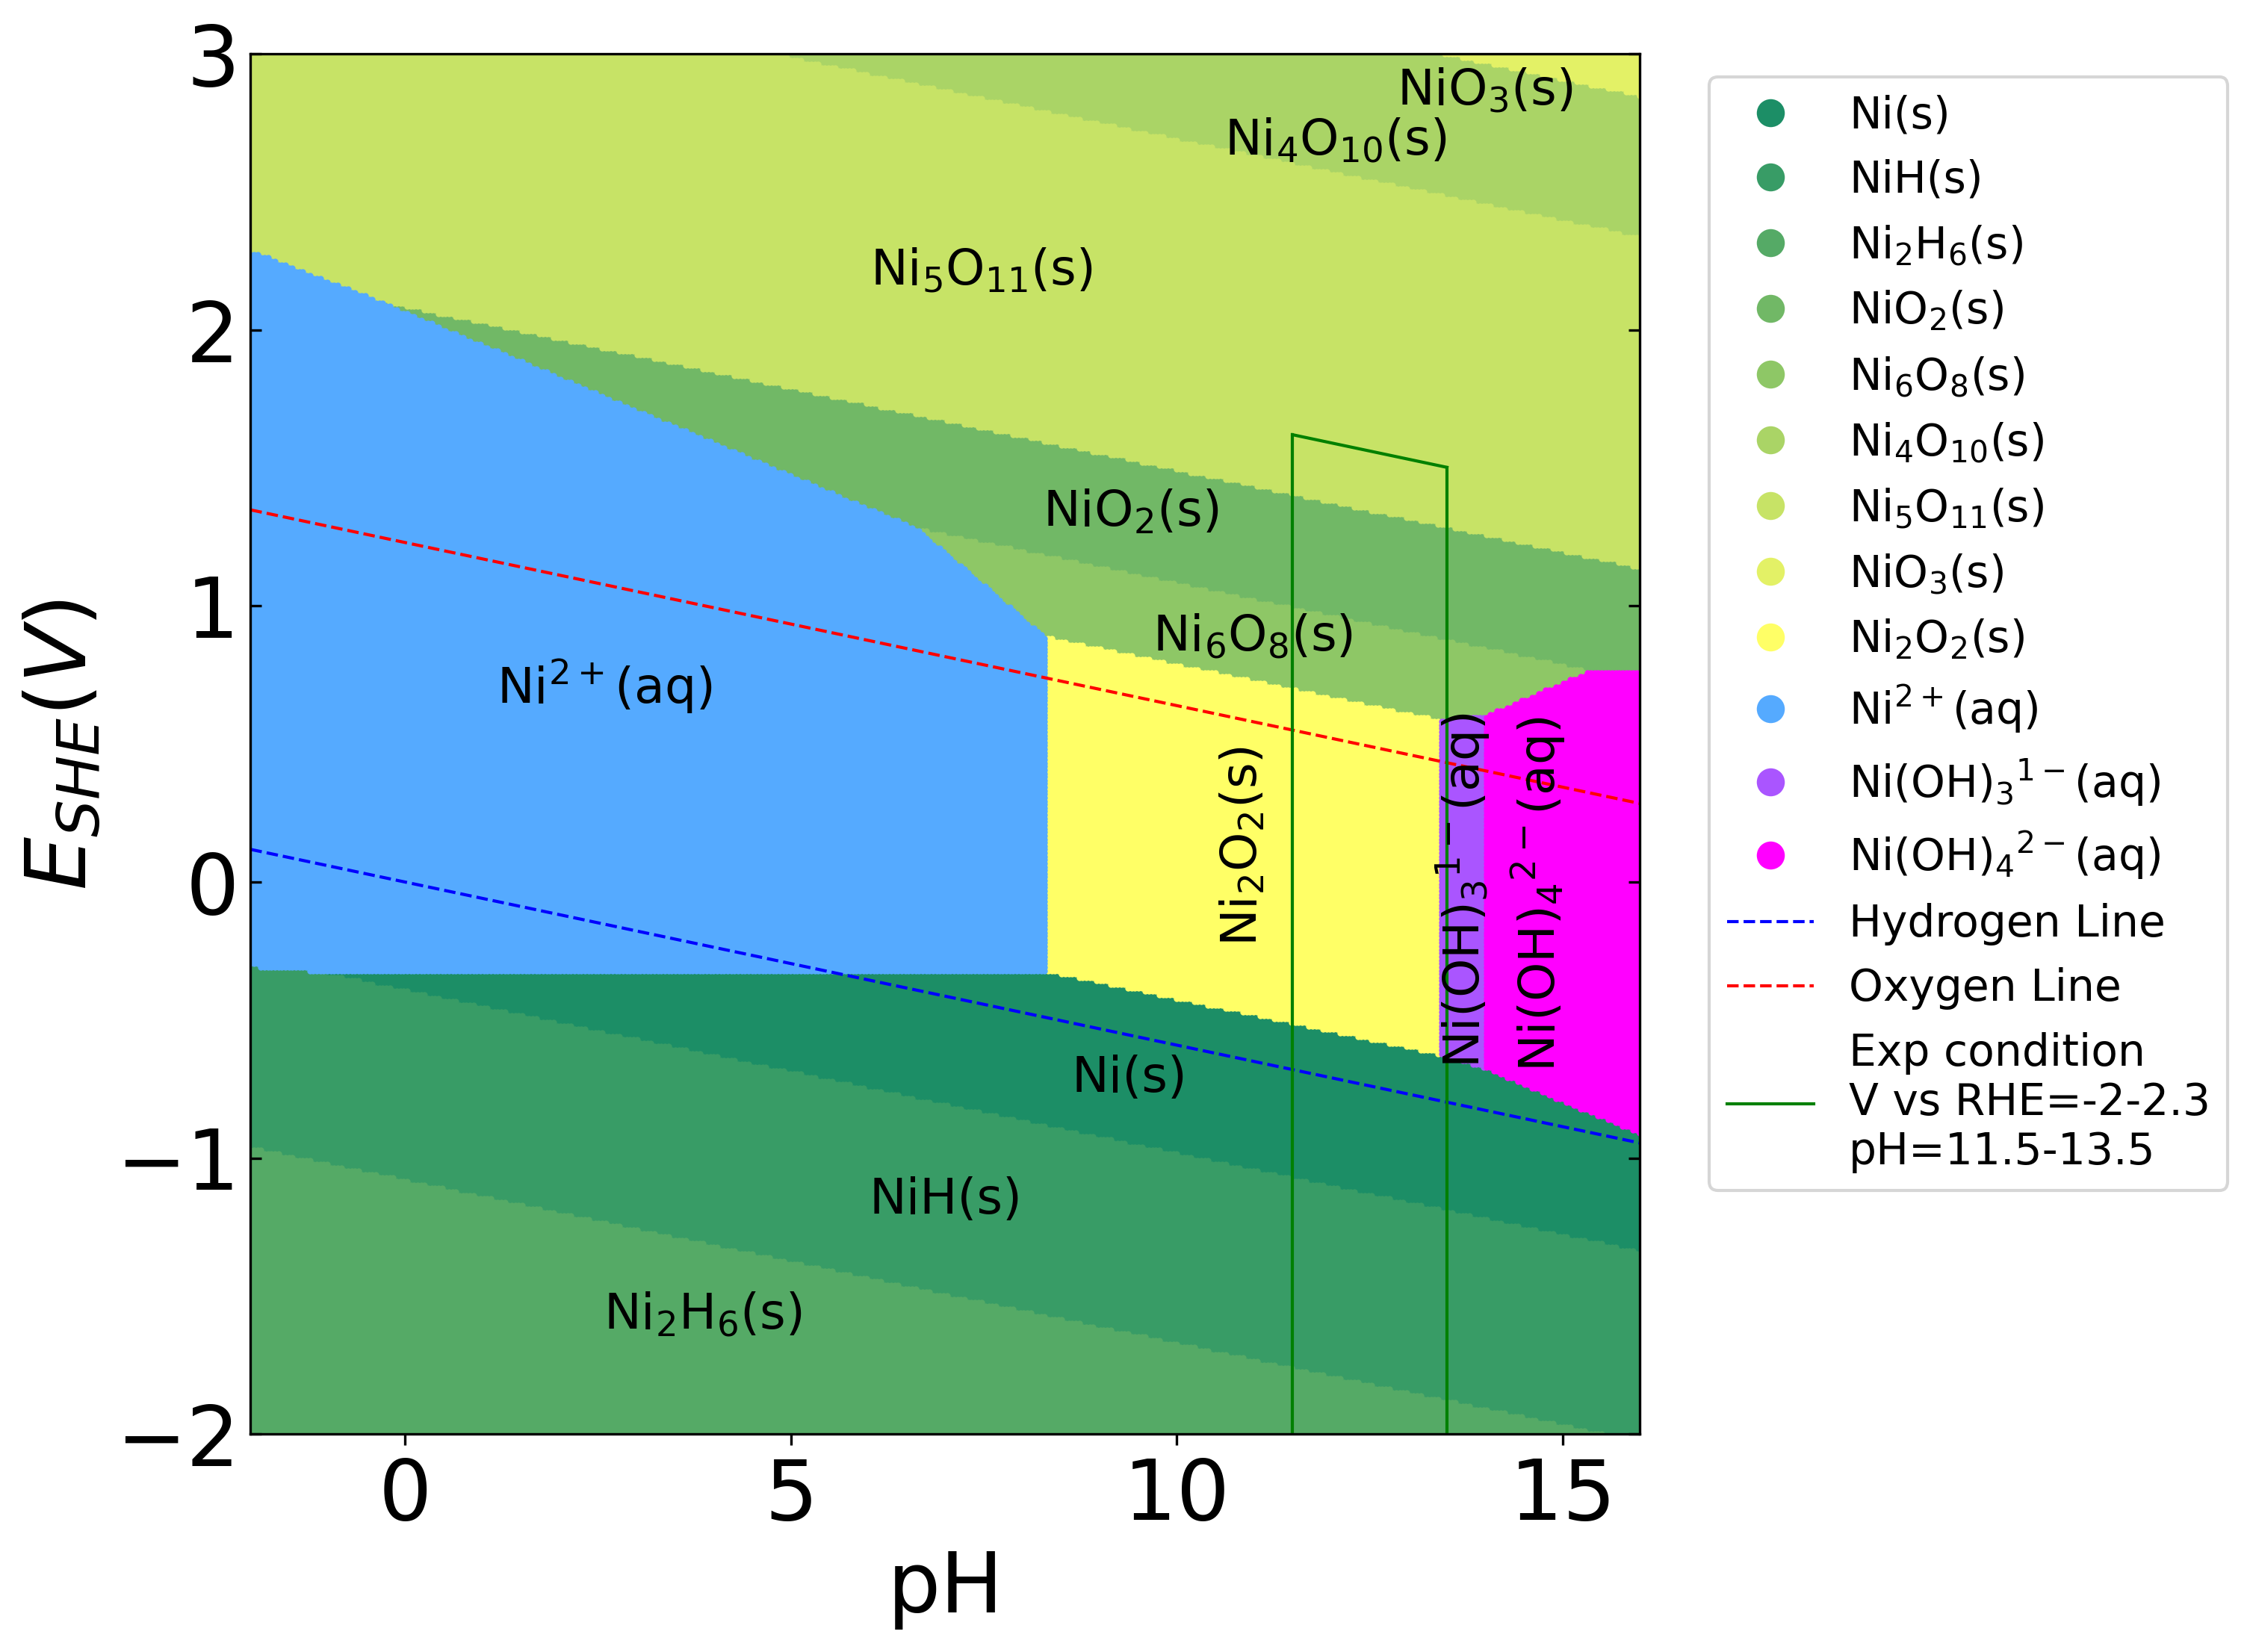
\includegraphics[width=\textwidth]{Figures/pourbaix_diagrams/Ni-NH3-H2O_activity=1e-04_[NH3]=0M_[Gly]=0M_[CN]=0.png}
%         \par\medskip
%     \end{subfigure}
%     % Subfigure (b)
%     \begin{subfigure}[b]{0.3\textwidth}
%         \subcaption{}\label{fig:Au_Pourbaix_H2O}
%         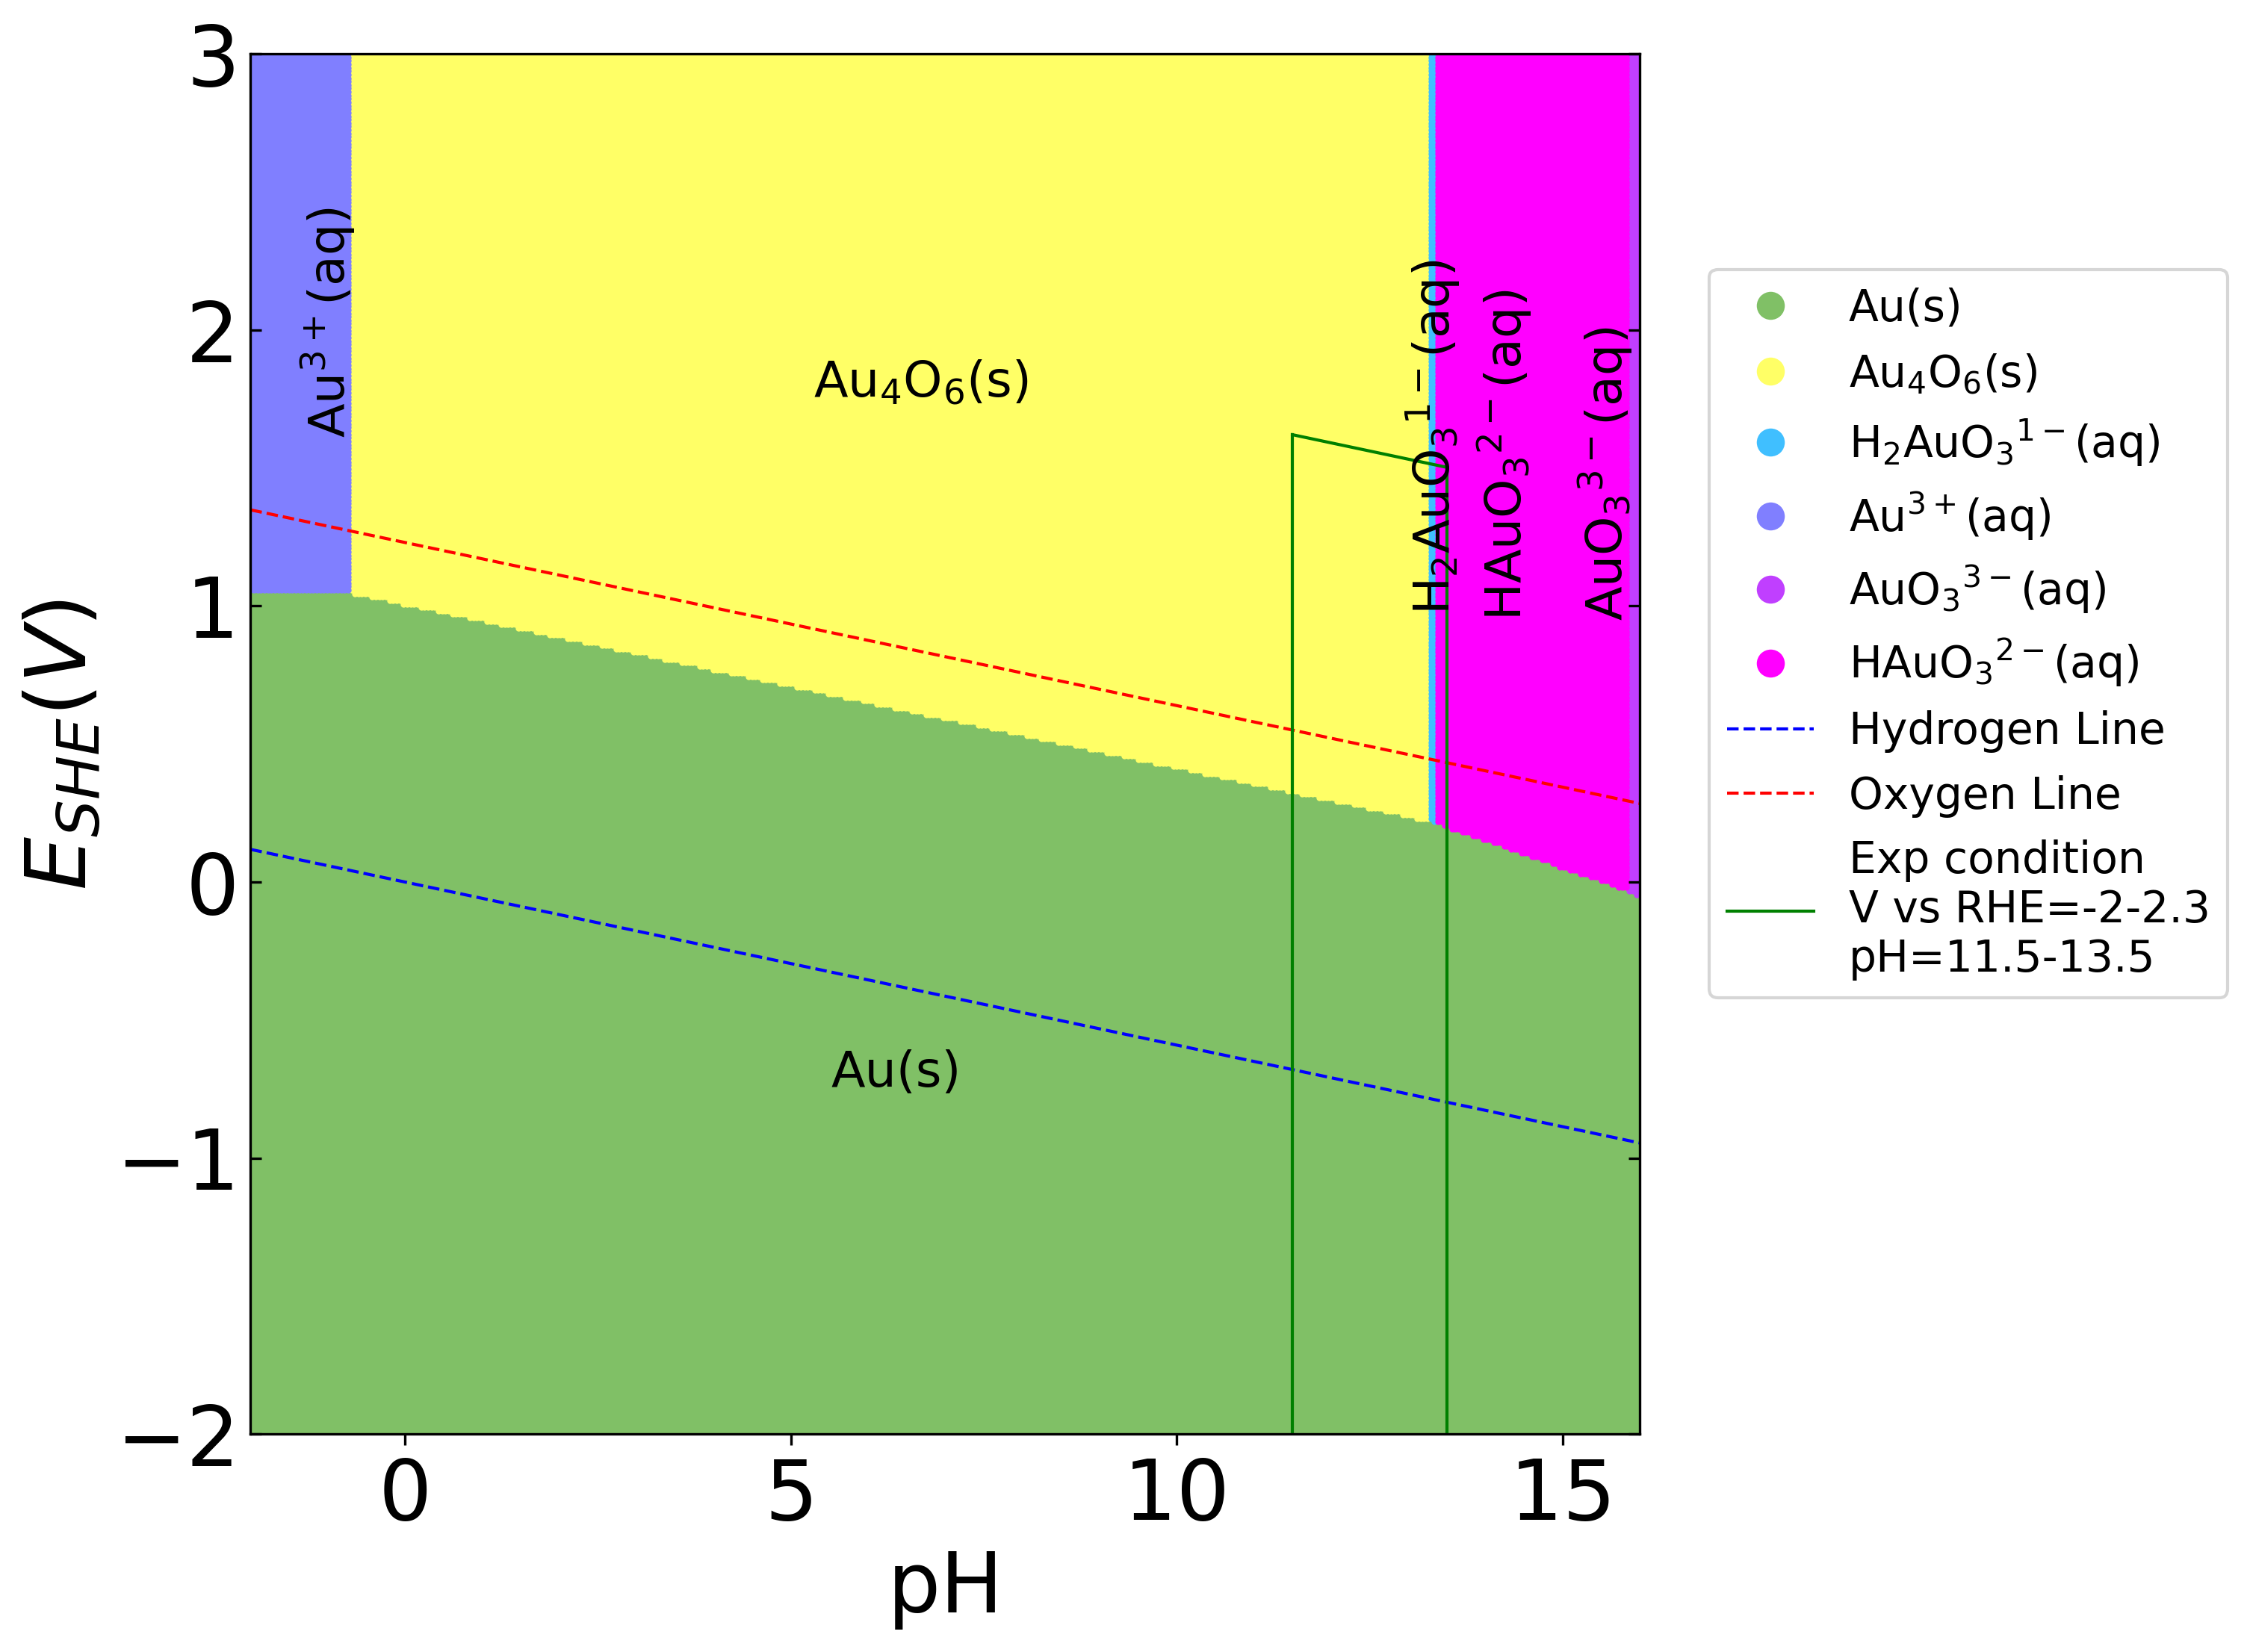
\includegraphics[width=\textwidth]{Figures/pourbaix_diagrams/Au-NH3-H2O_activity=1e-04_[NH3]=0M_[Gly]=0M_[CN]=0.png}
%         \par\medskip
%     \end{subfigure}
%     % Subfigure (c)
%     \begin{subfigure}[b]{0.3\textwidth}
%         \subcaption{}\label{fig:Cu_Pourbaix_H2O}
%         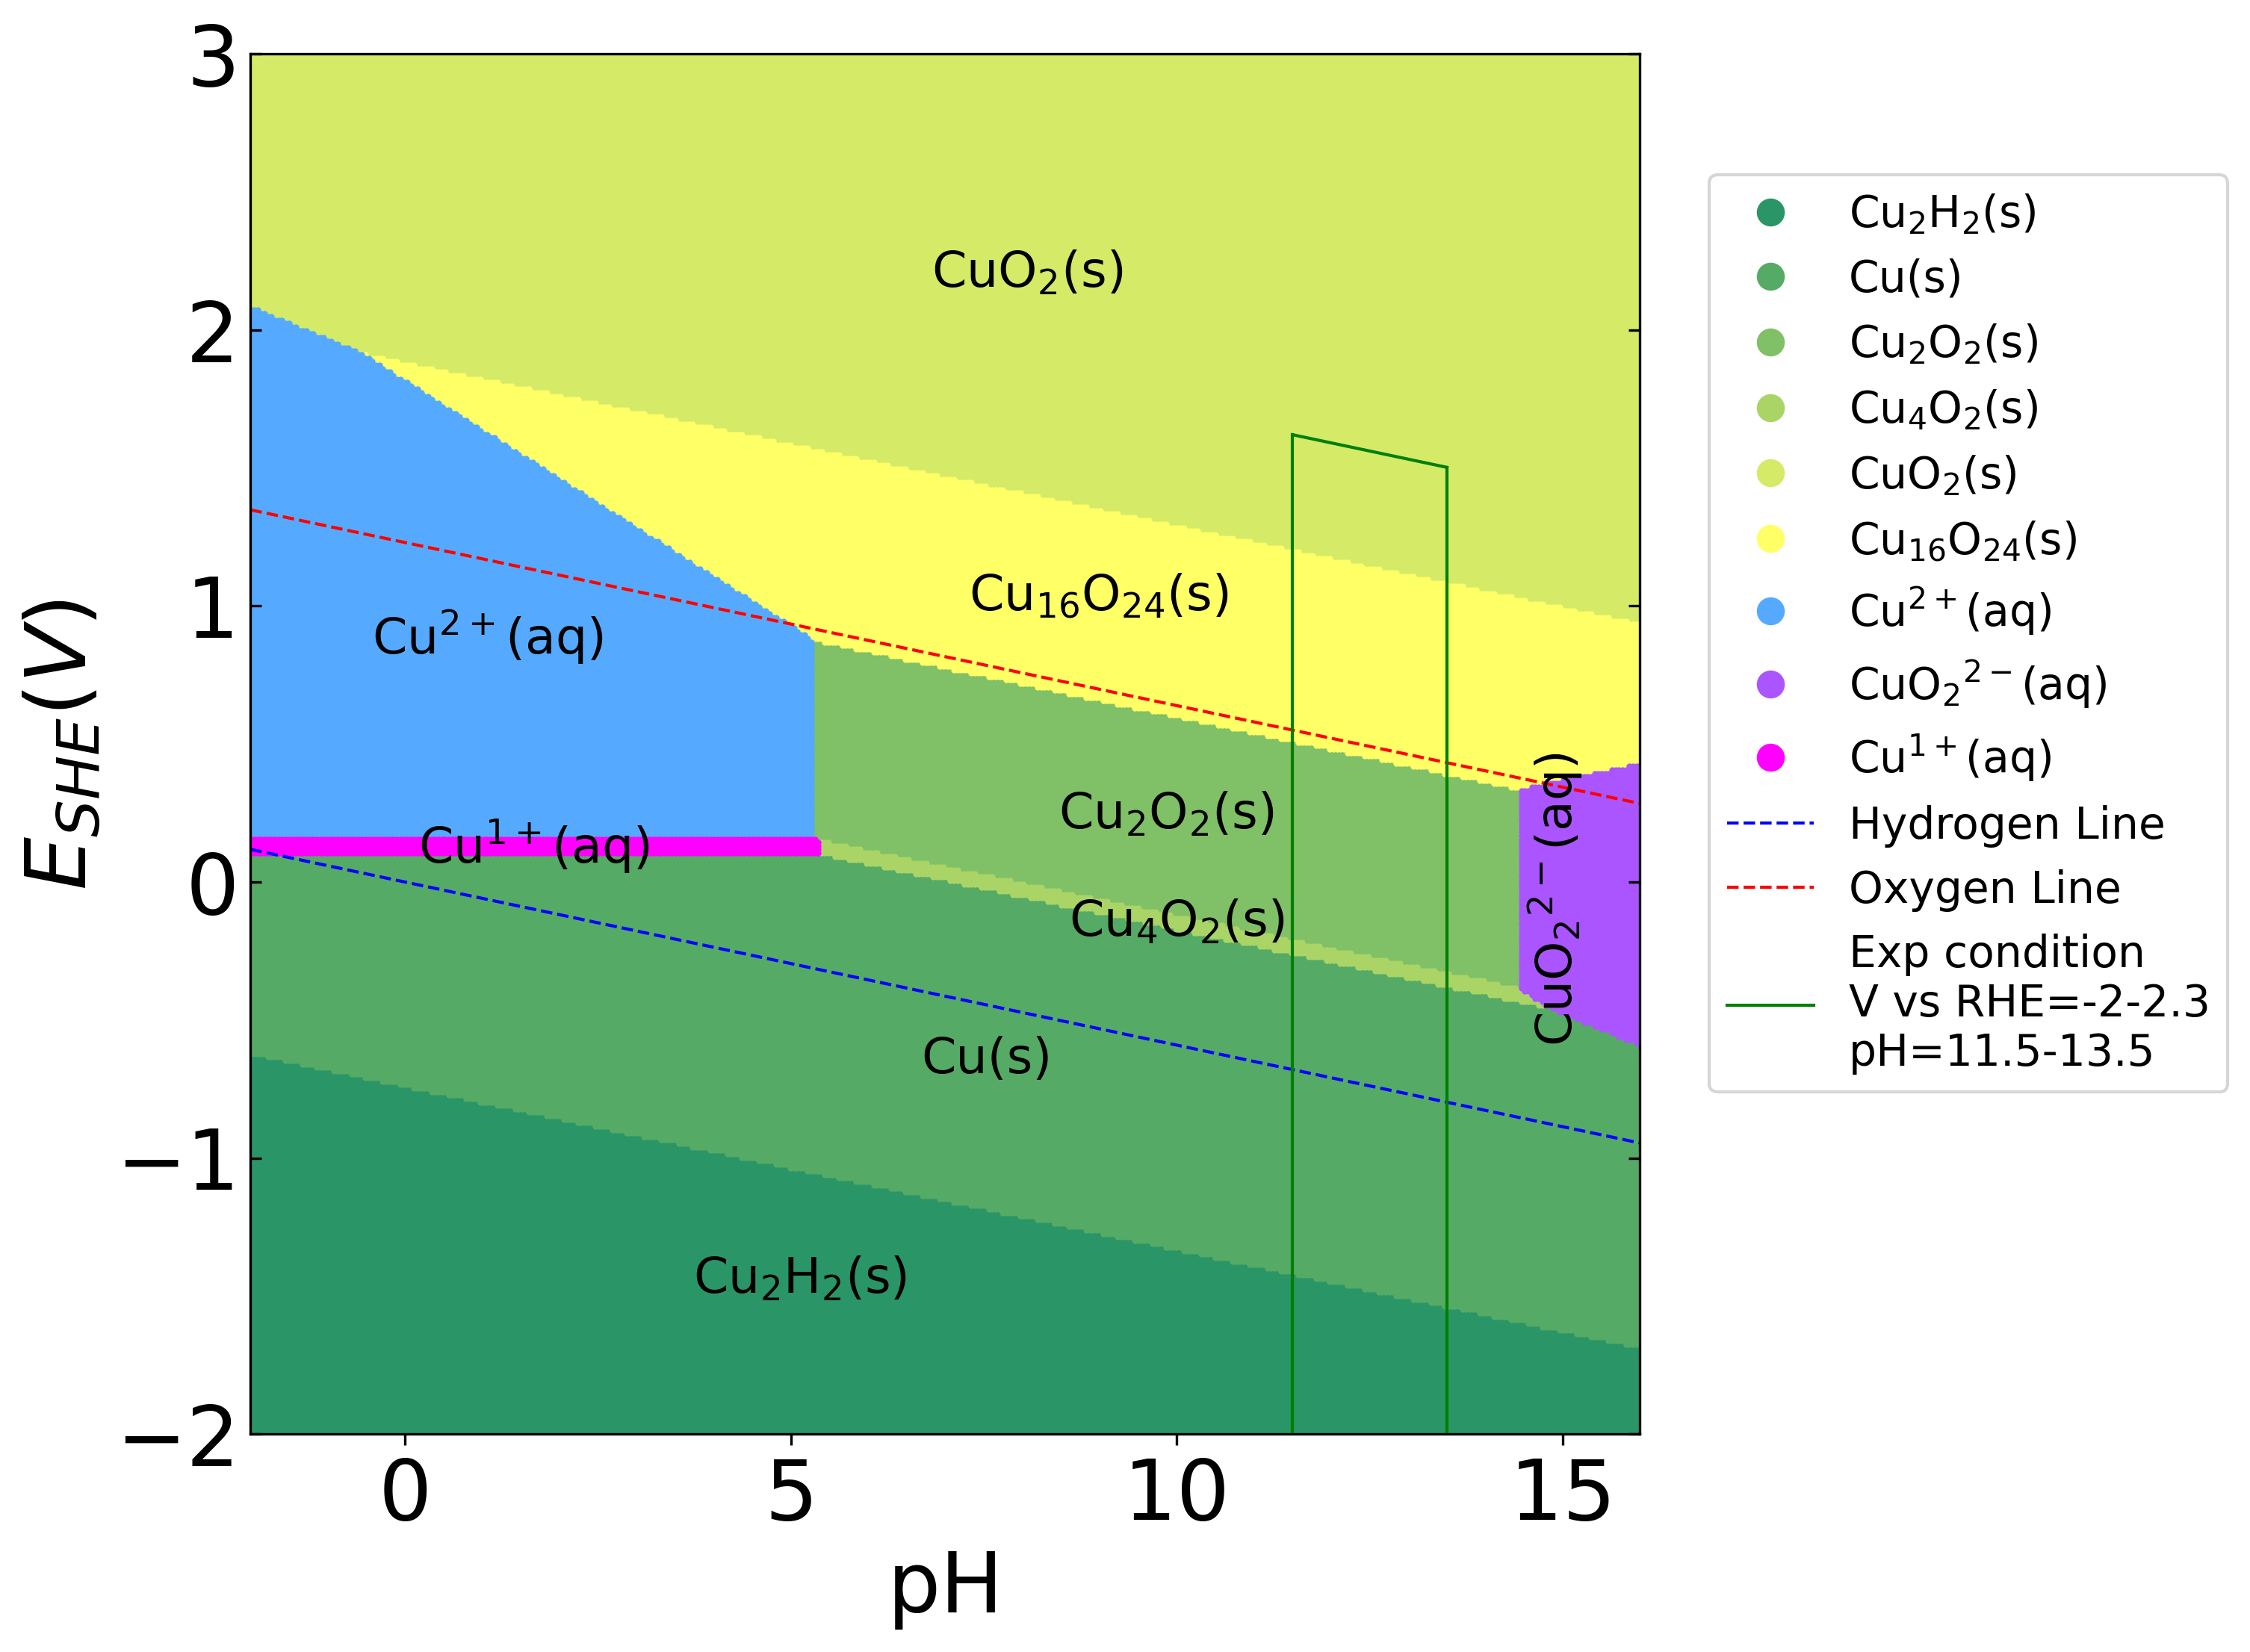
\includegraphics[width=\textwidth]{Figures/pourbaix_diagrams/Cu-NH3-H2O_activity=1e-04_[NH3]=0M_[Gly]=0M_[CN]=0.png}
%         \par\medskip   
%     \end{subfigure}
%     % Subfigure (d)
%     \begin{subfigure}[b]{0.3\textwidth}
%         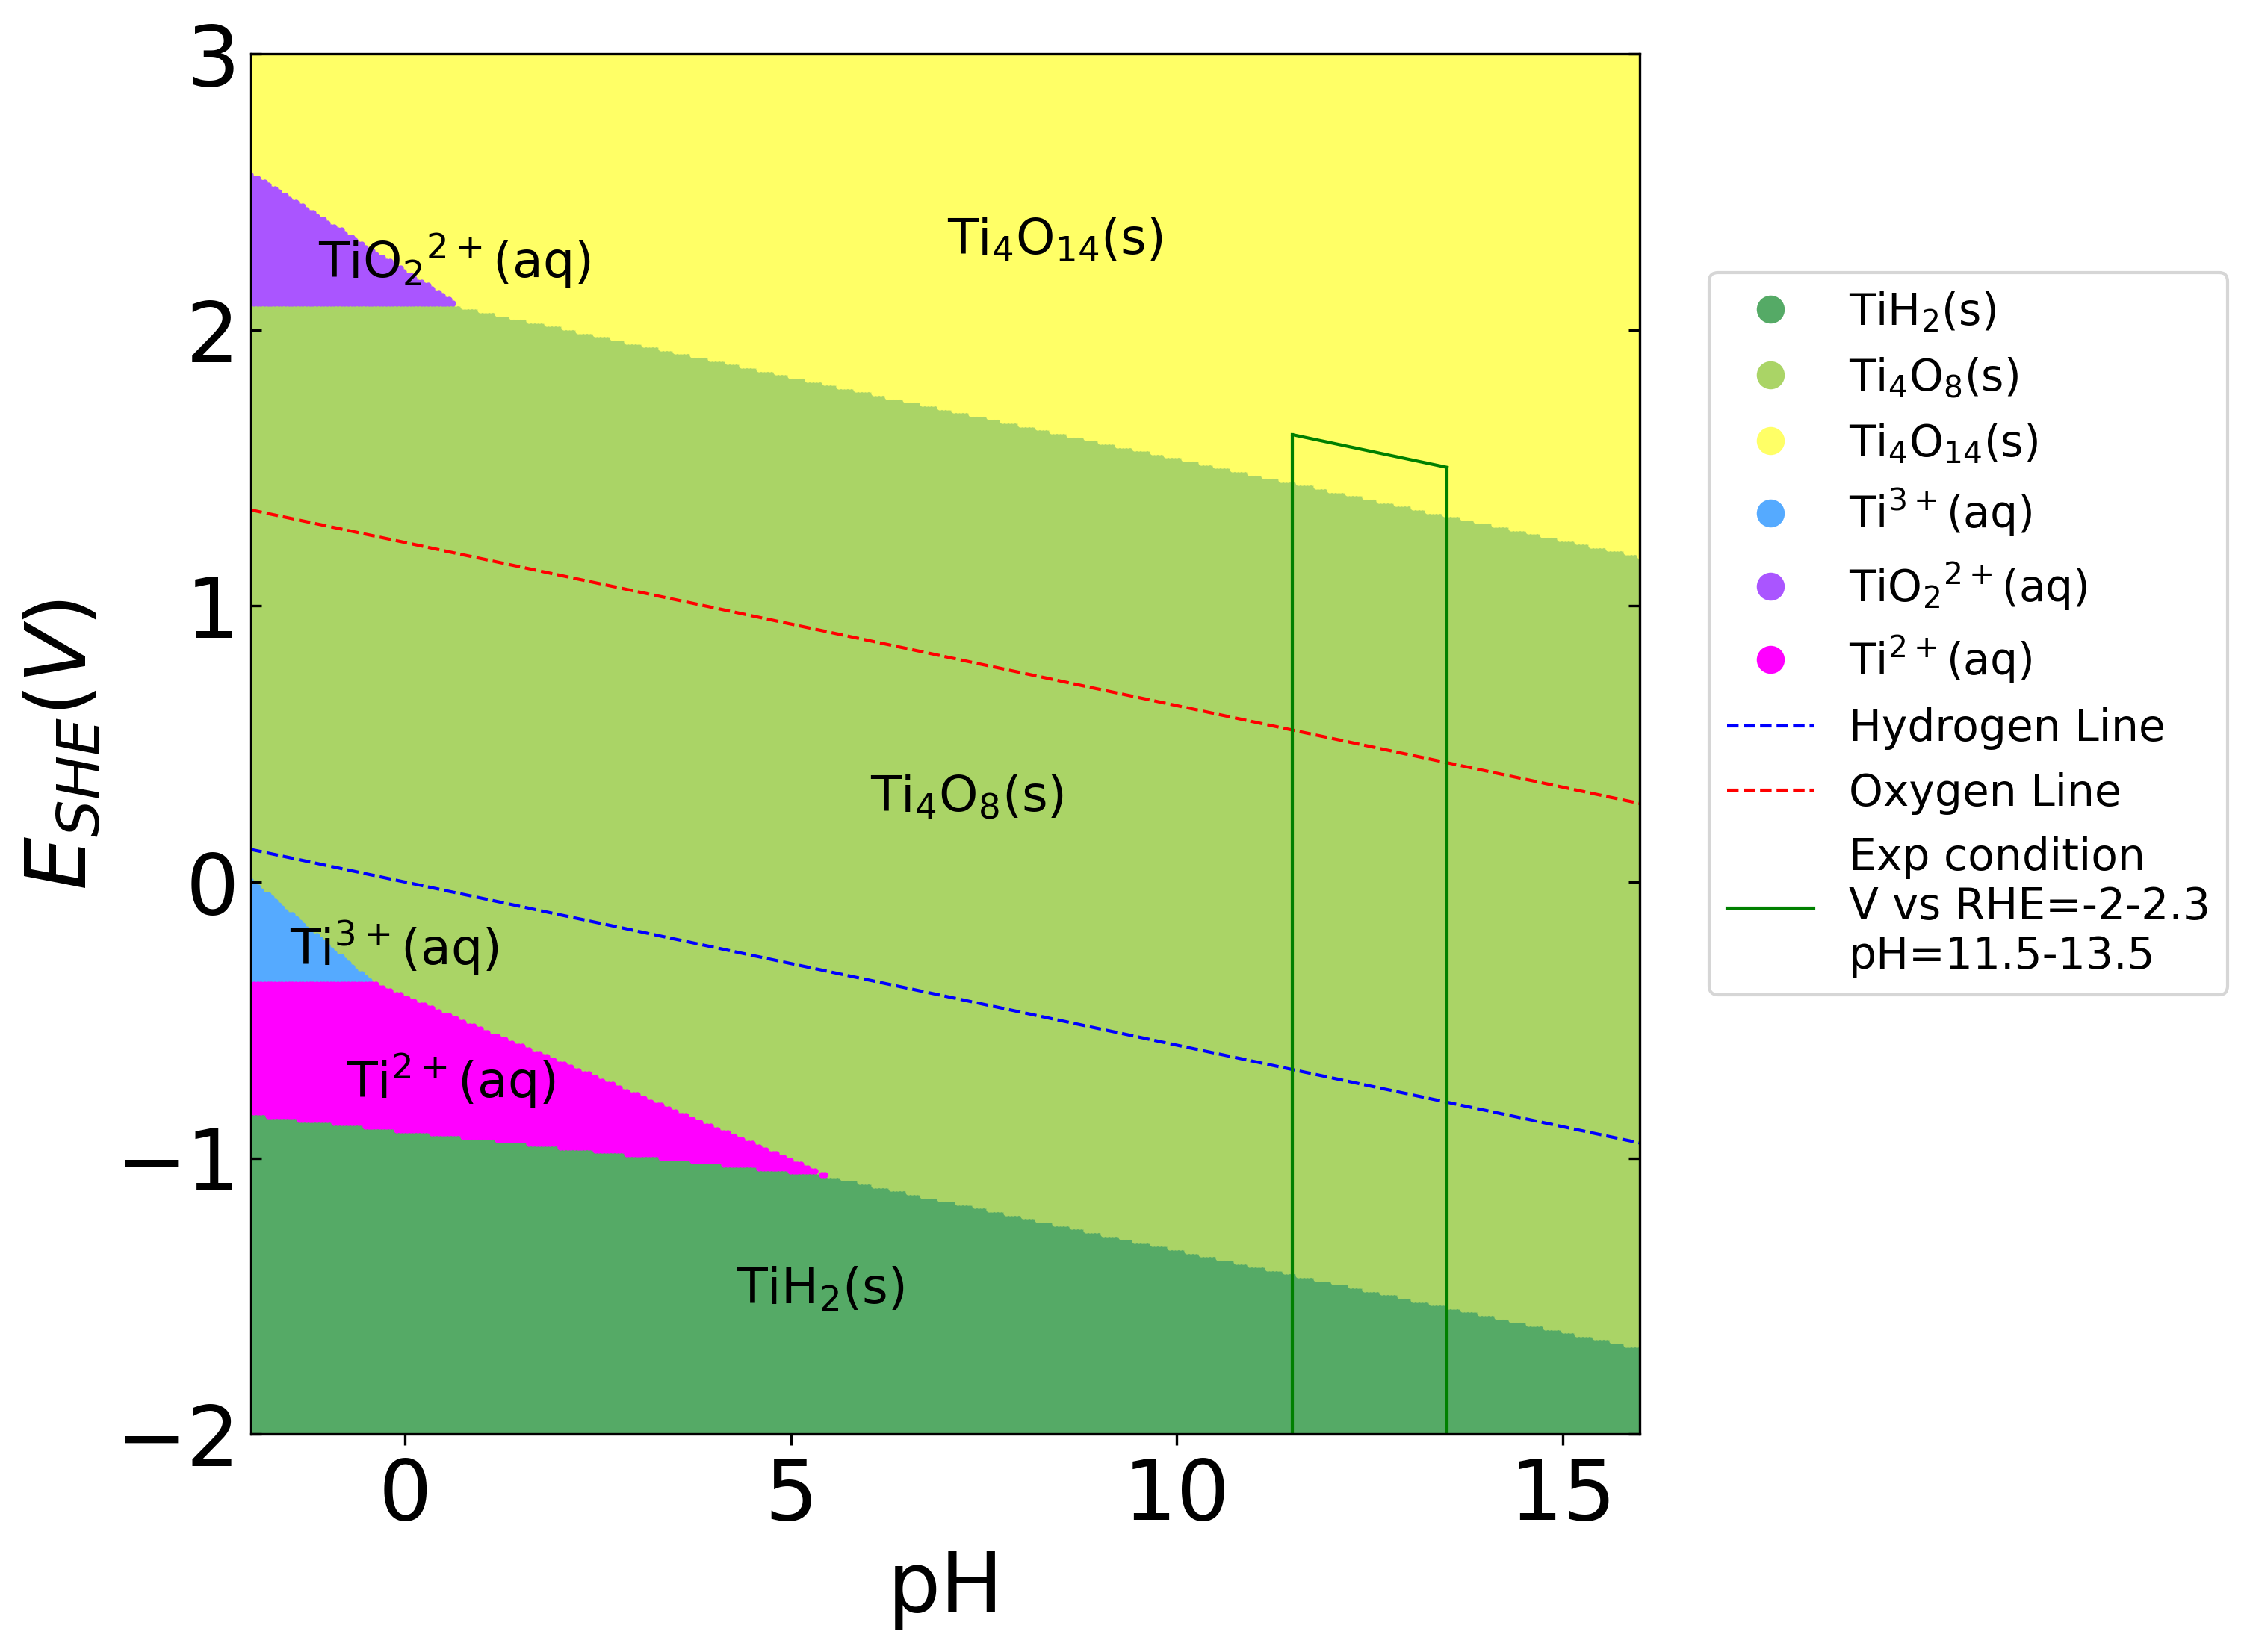
\includegraphics[width=\textwidth]{Figures/pourbaix_diagrams/Ti-NH3-H2O_activity=1e-04_[NH3]=0M_[Gly]=0M_[CN]=0.png}
%         \subcaption{}\label{fig:Ti_Pourbaix_H2O}
%     \end{subfigure}
%     % Subfigure (e)
%     \begin{subfigure}[b]{0.3\textwidth}
%         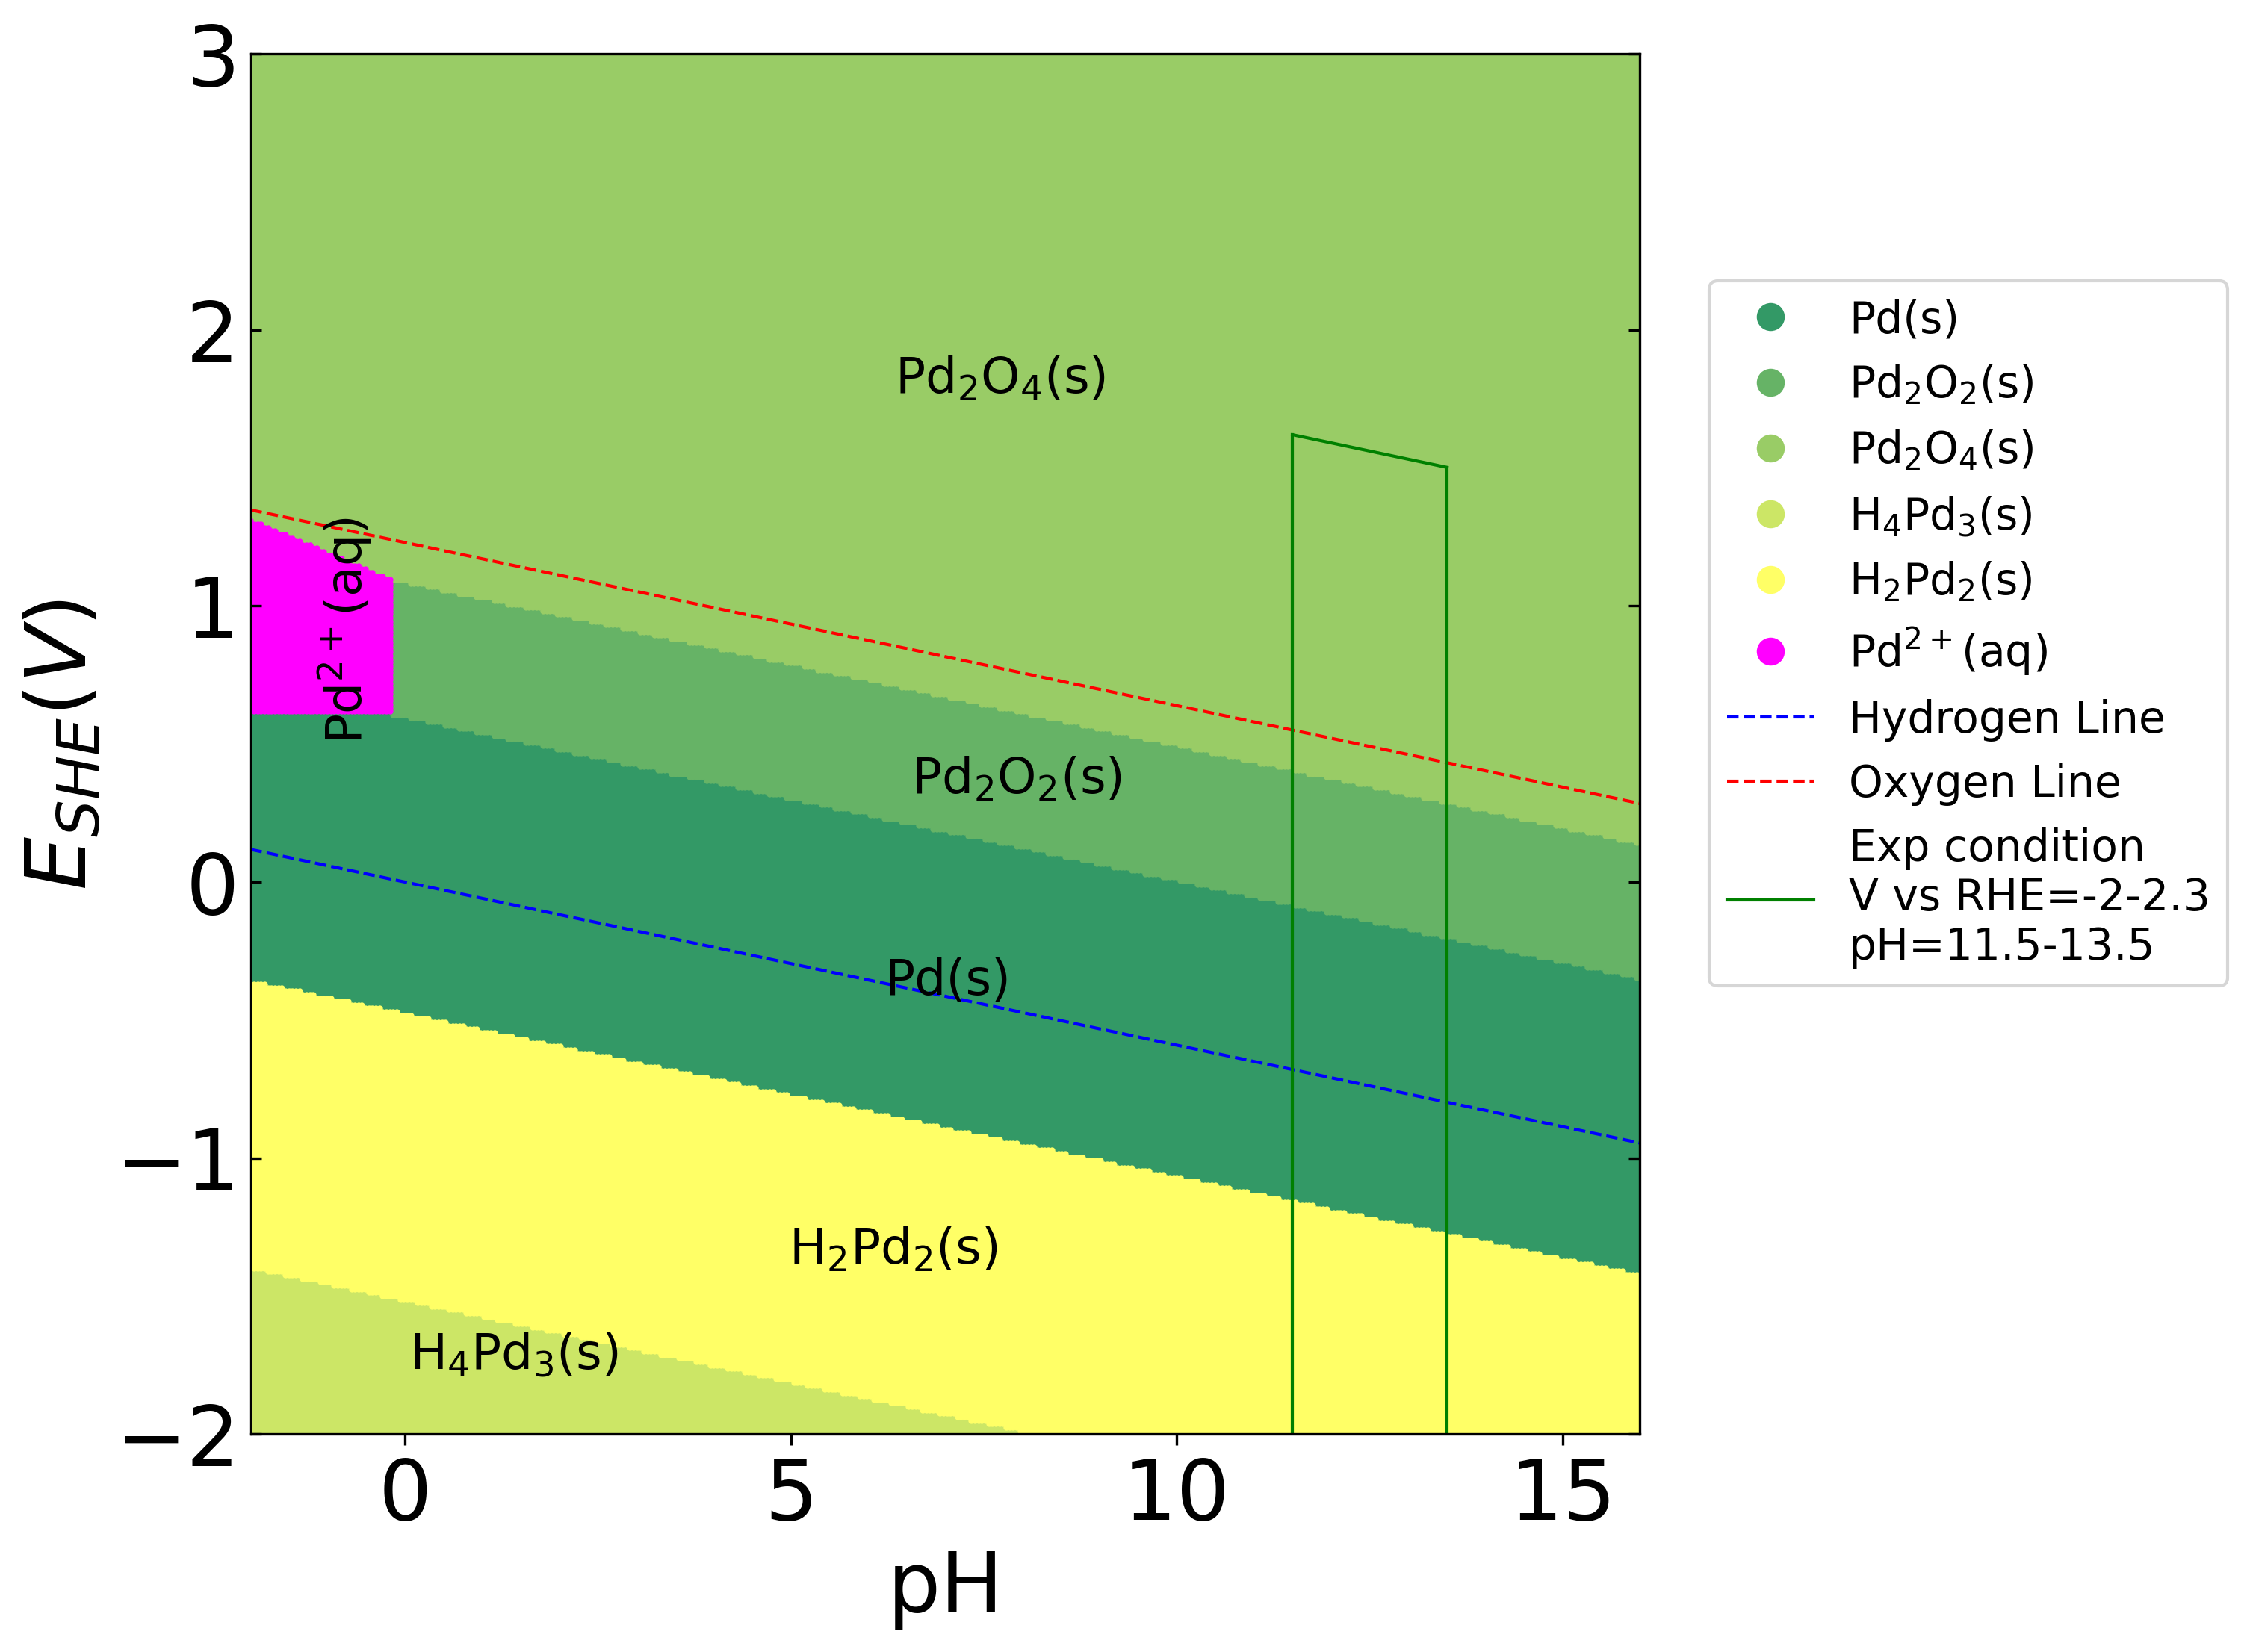
\includegraphics[width=\textwidth]{Figures/pourbaix_diagrams/Pd-NH3-H2O_activity=1e-04_[NH3]=0M_[Gly]=0M_[CN]=0.png}
%         \subcaption{}\label{fig:Pd_Pourbaix_H2O}
%     \end{subfigure}
%     % Subfigure (f)
%     \begin{subfigure}[b]{0.3\textwidth}
%         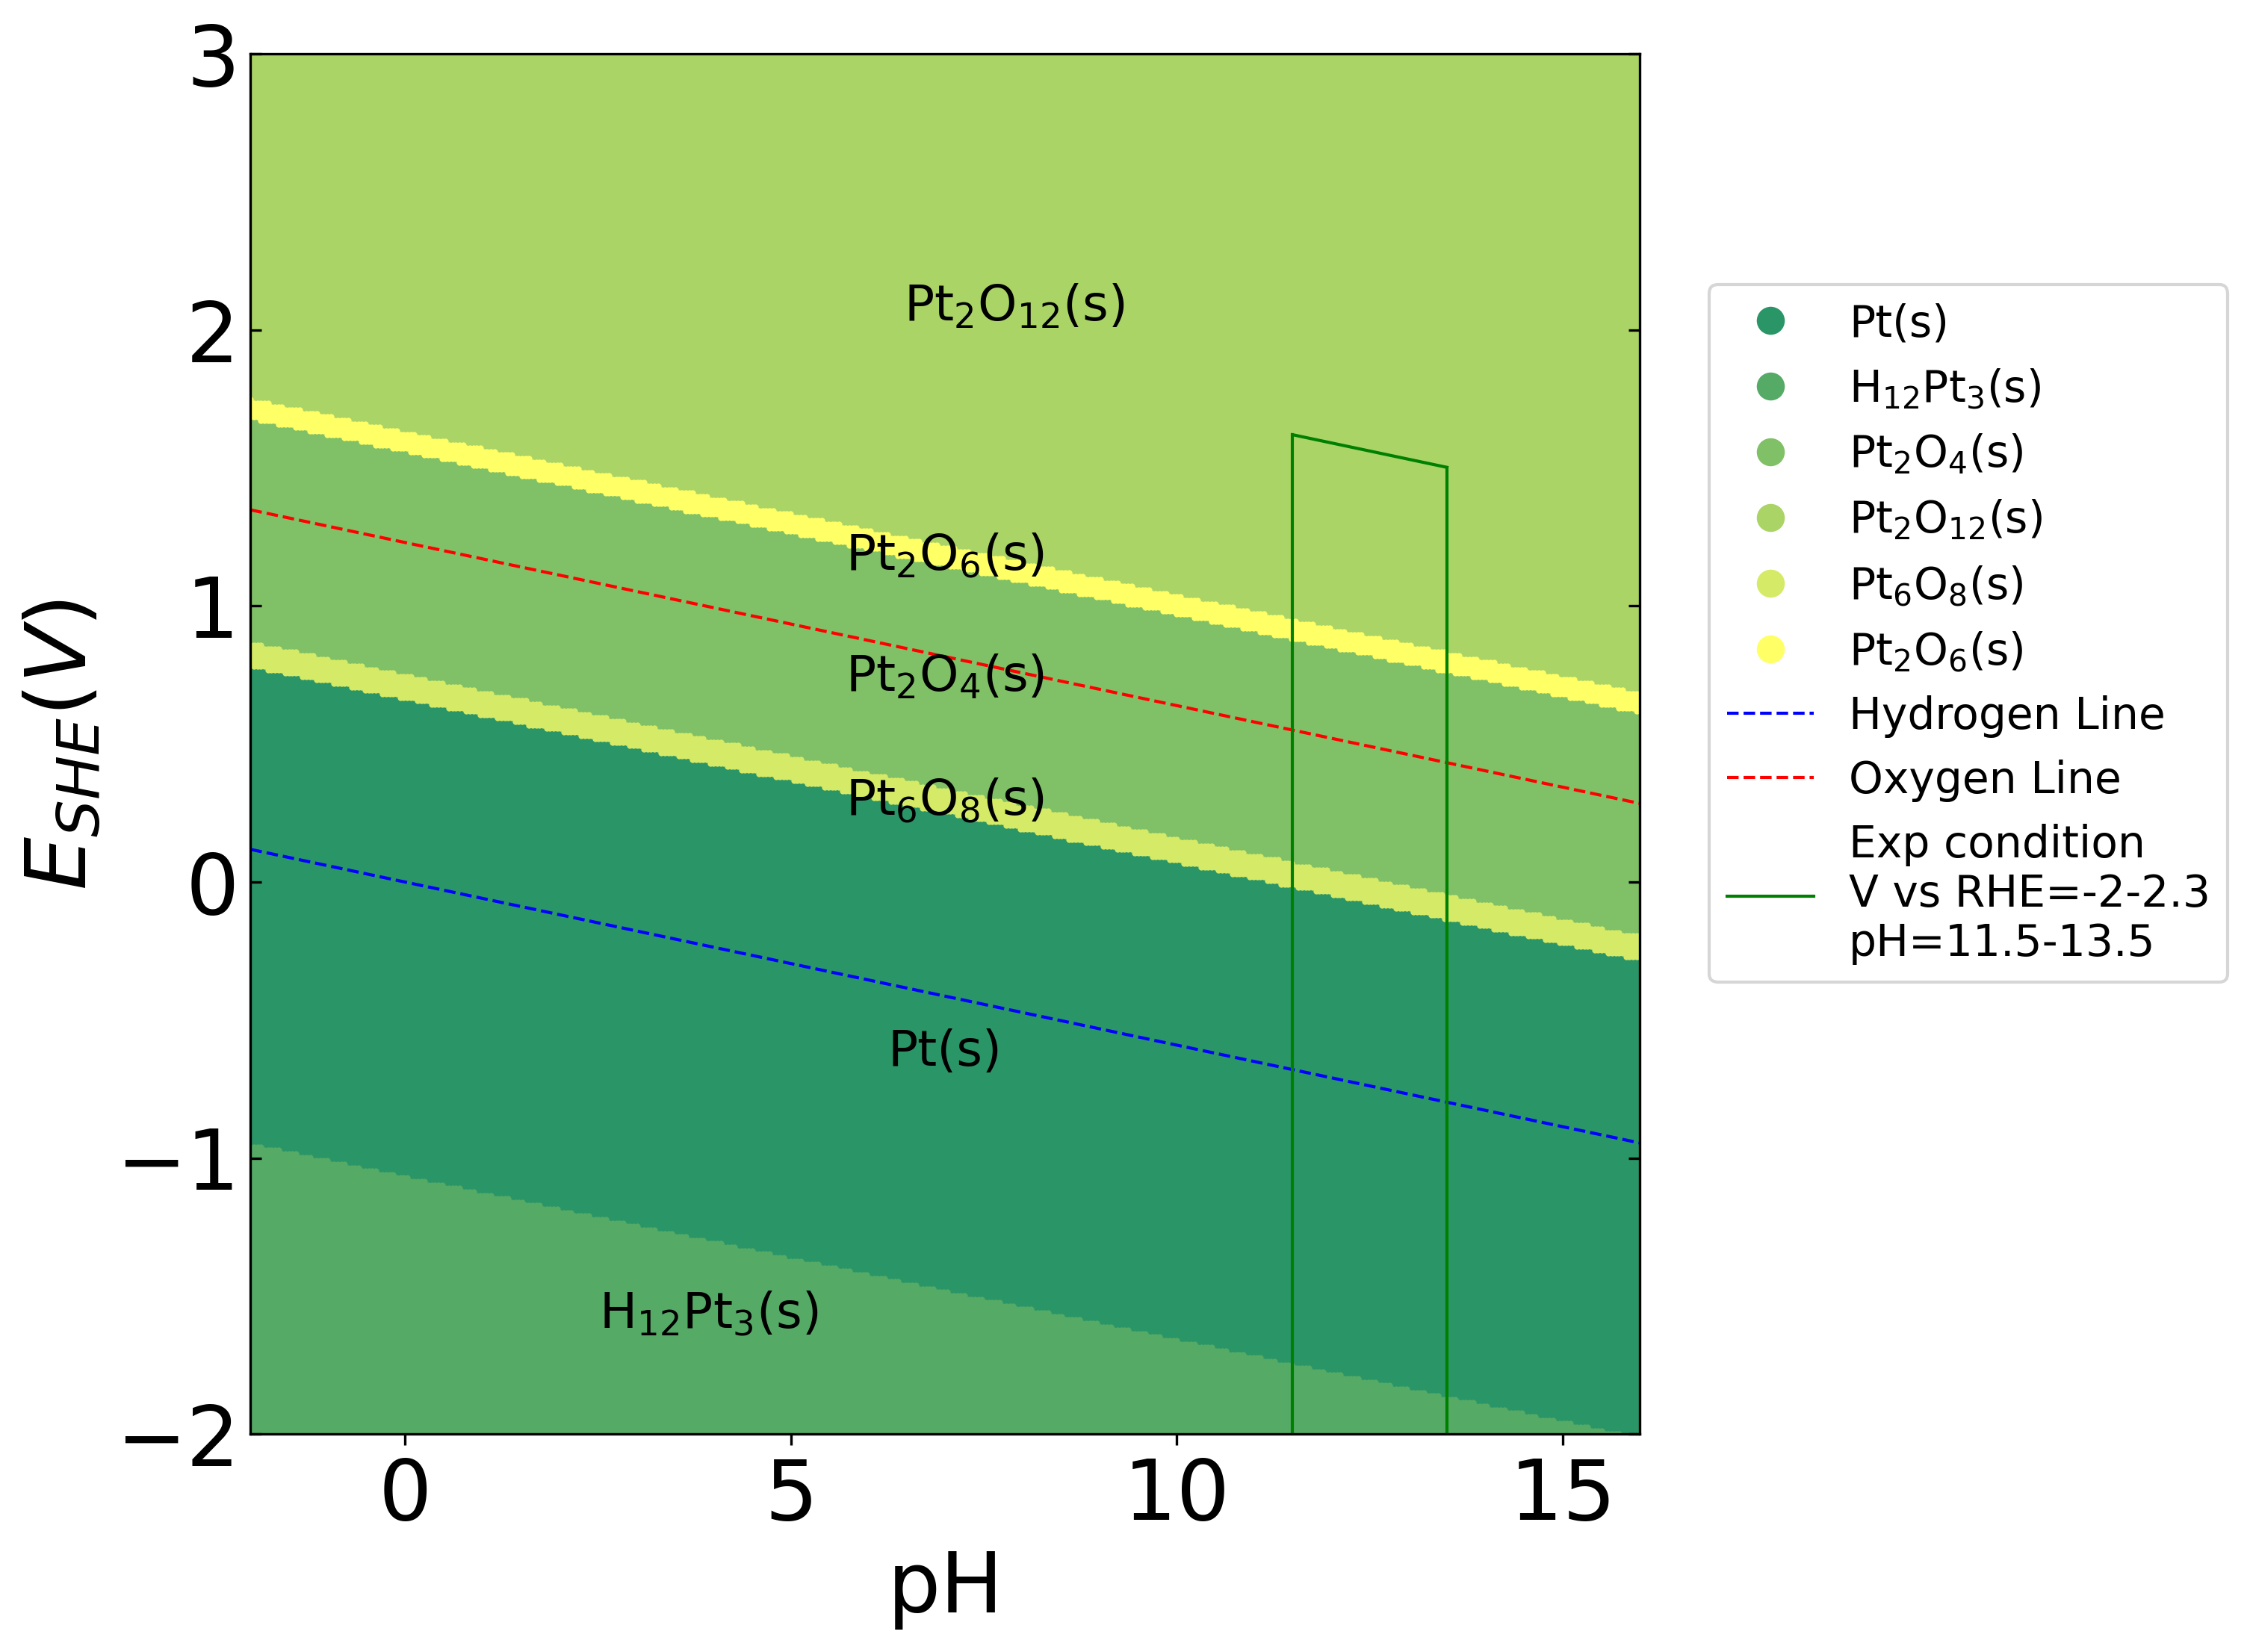
\includegraphics[width=\textwidth]{Figures/pourbaix_diagrams/Pt-NH3-H2O_activity=1e-04_[NH3]=0M_[Gly]=0M_[CN]=0.png}
%         \subcaption{}\label{fig:Pt_Pourbaix_H2O}
%     \end{subfigure}

%     \caption{Pourbaix diagrams for metal-\ce{H2O} systems. Green box indicates experimental condition at applied potential vs RHE = -2 to 2V, pH = 11.5 to 13.5.}
%     \label{fig:Pourbaix_NH3_Gly}
% \end{figure}

%%%%%%%%%%%%%%%%%%%%%%%%%%%%%%%%% NH3, Gly and CN- %%%%%%%%%%%%%%%%%%%%%%%%%%%%%%%%%
% \begin{figure}[htbp]
%     \centering
%     % Subfigure (a)
%     \begin{subfigure}[b]{0.3\textwidth}
%         \subcaption{}\label{fig:Ni_Pourbaix_CN_CH3_Gly}
%         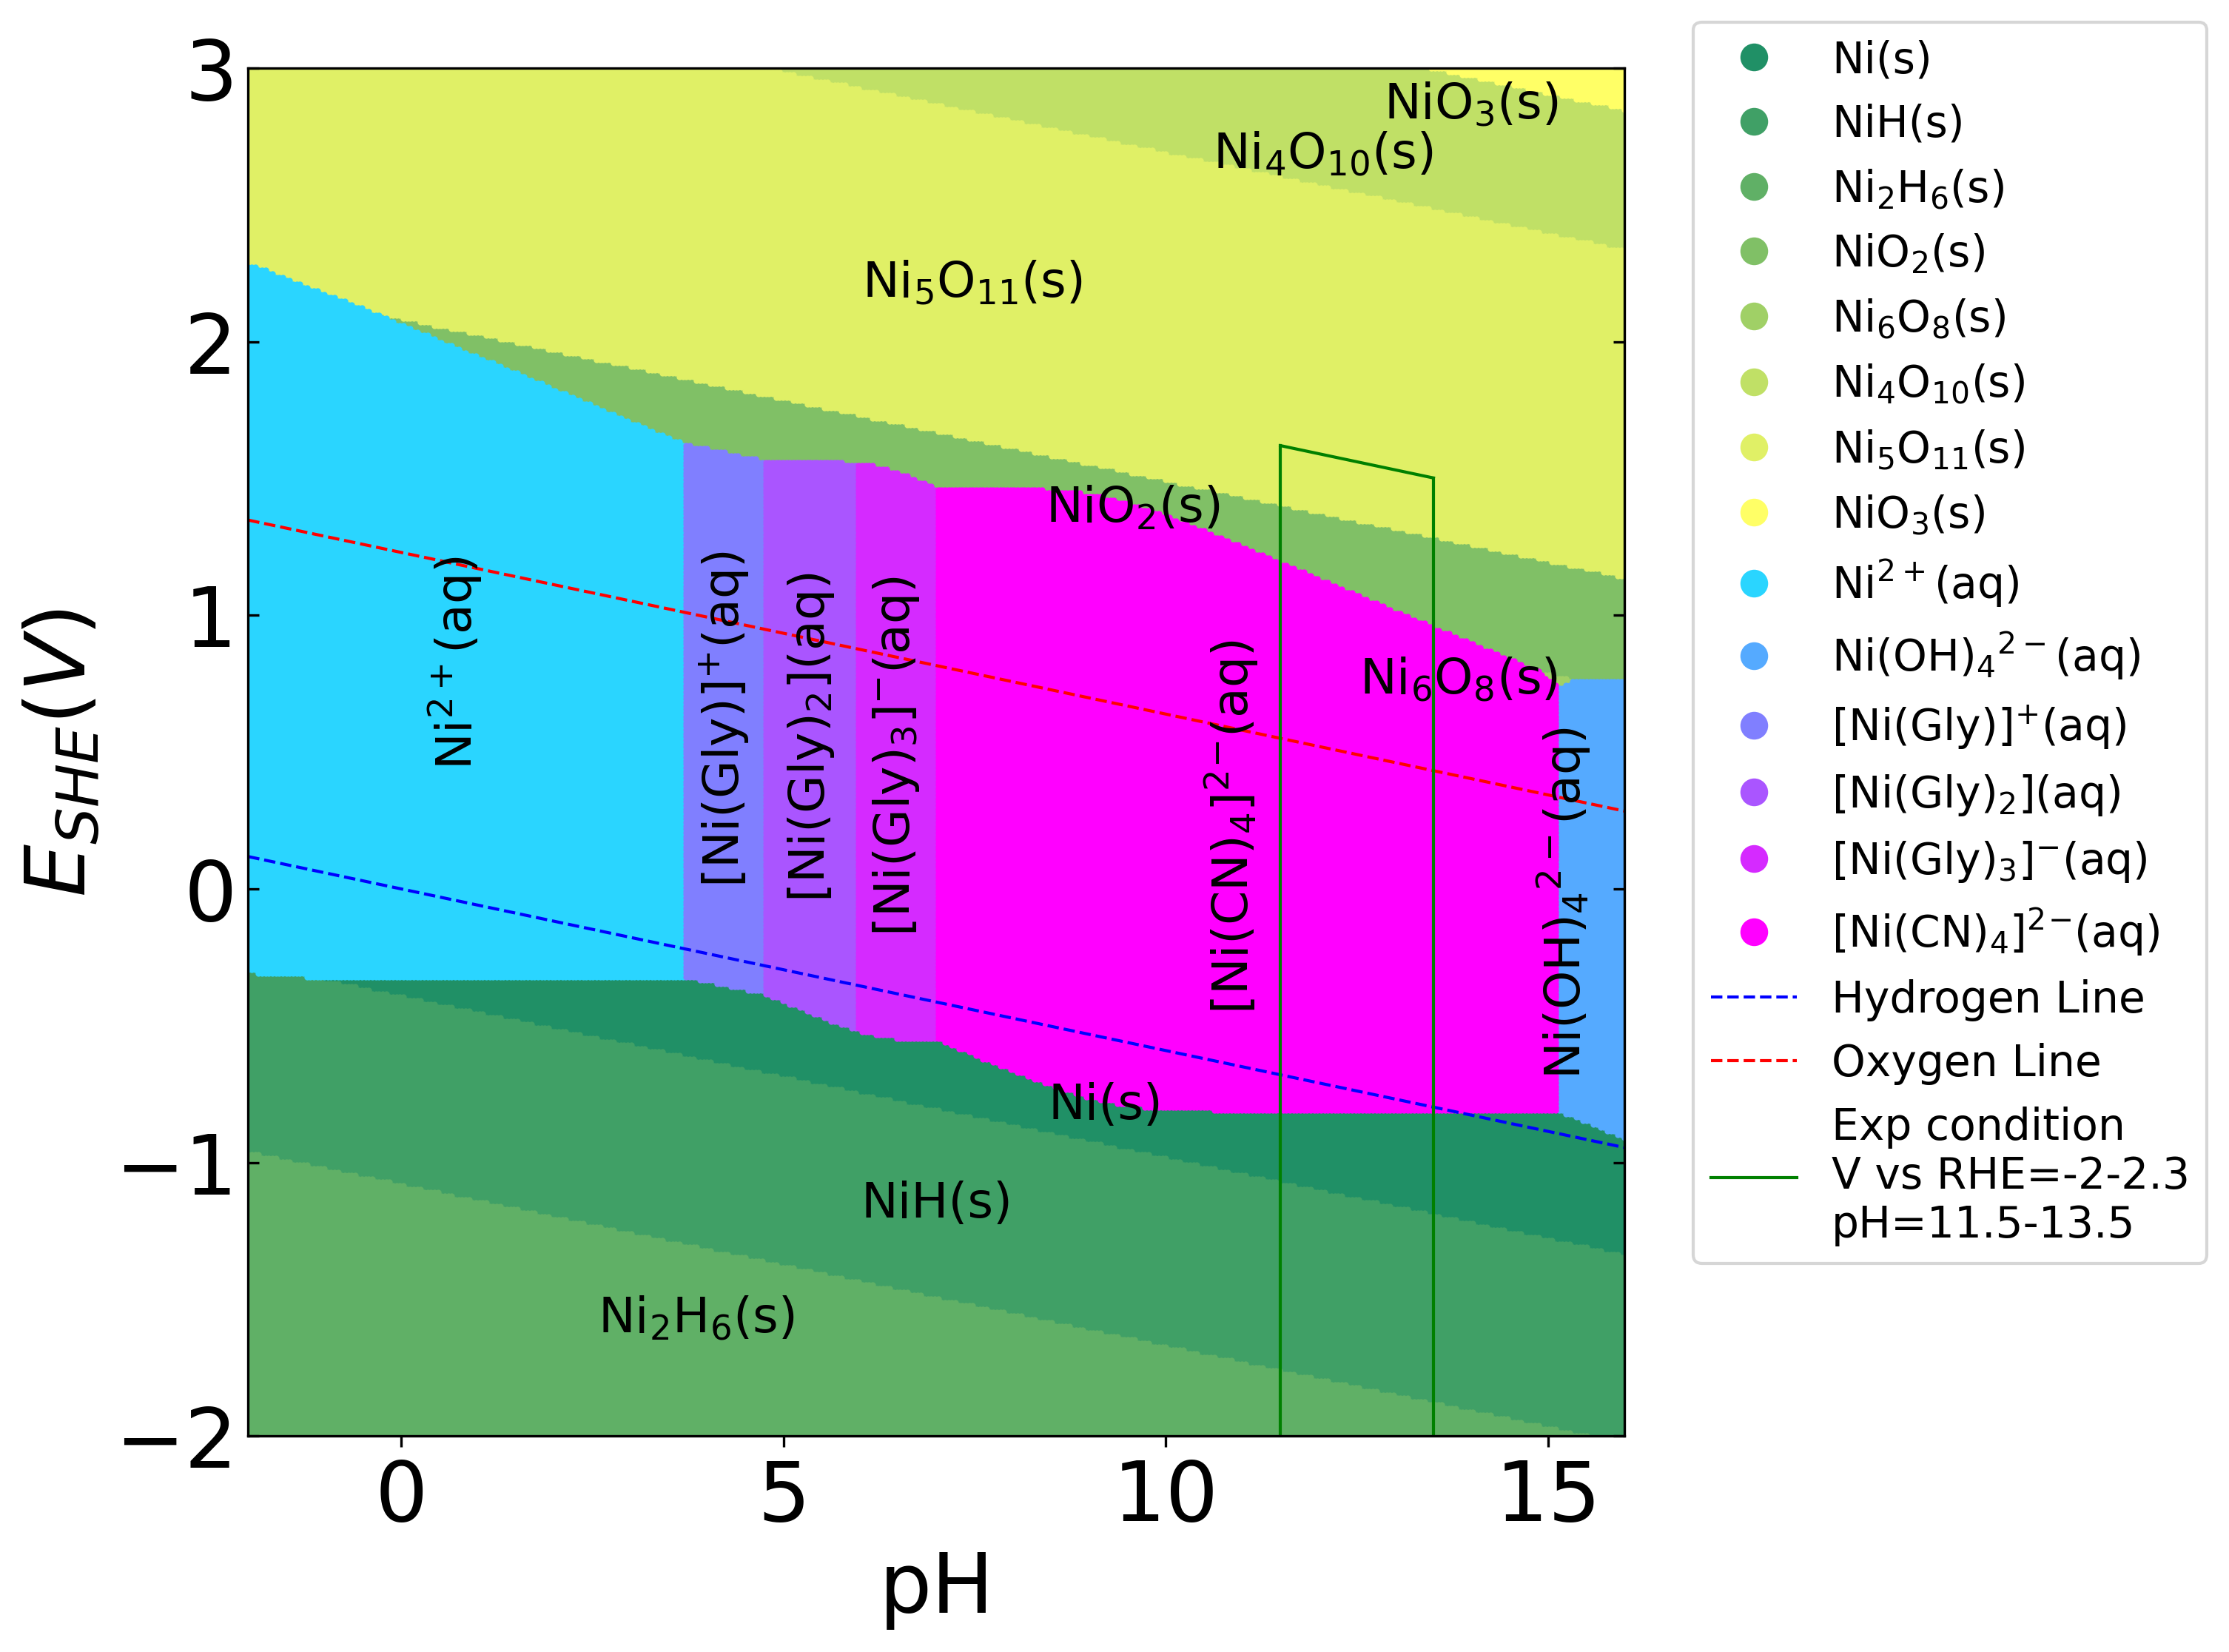
\includegraphics[width=\textwidth]{Figures/pourbaix_diagrams/Ni-NH3-H2O_activity=1e-04_[NH3]=0.02M_[Gly]=0.005M_[CN]=0.0001.png}
%         \par\medskip
%     \end{subfigure}
%     % Subfigure (b)
%     \begin{subfigure}[b]{0.3\textwidth}
%         \subcaption{}\label{fig:Au_Pourbaix_CN_CH3_Gly}
%         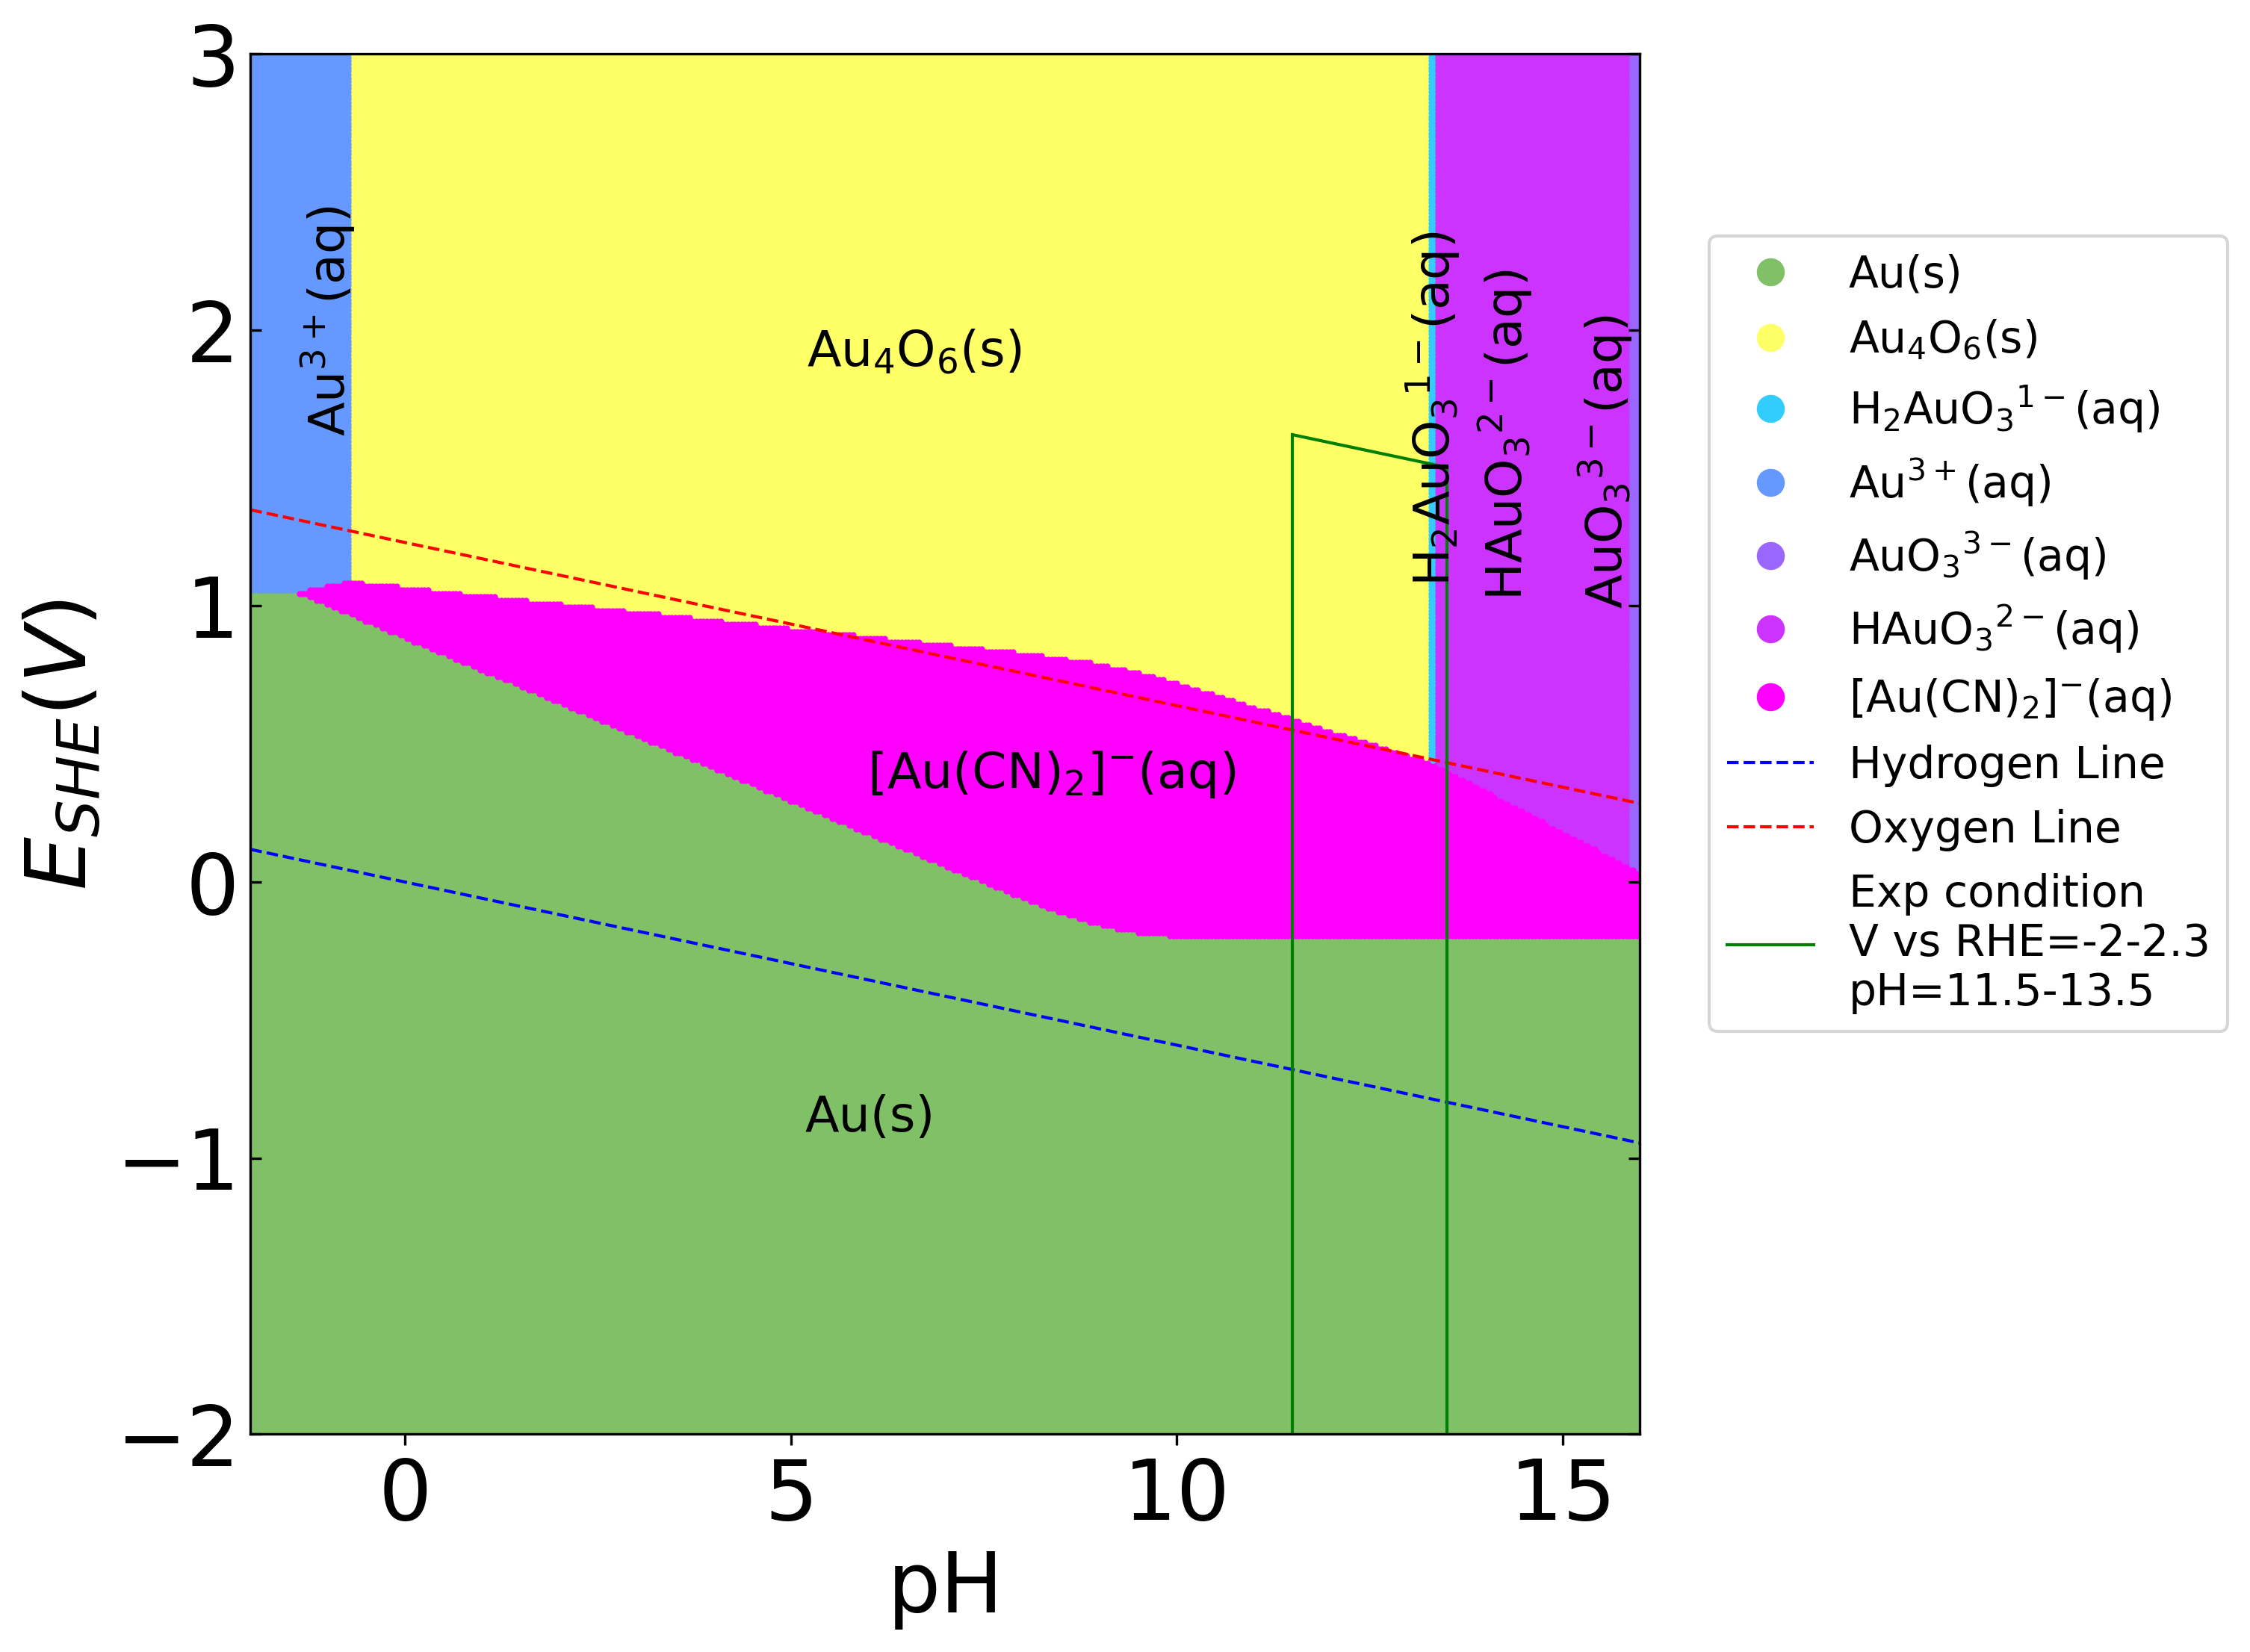
\includegraphics[width=\textwidth]{Figures/pourbaix_diagrams/Au-NH3-H2O_activity=1e-04_[NH3]=0.02M_[Gly]=0.005M_[CN]=0.0001.png}
%         \par\medskip
%     \end{subfigure}
%     % Subfigure (c)
%     \begin{subfigure}[b]{0.3\textwidth}
%         \subcaption{}\label{fig:Cu_Pourbaix_CN_CH3_Gly}
%         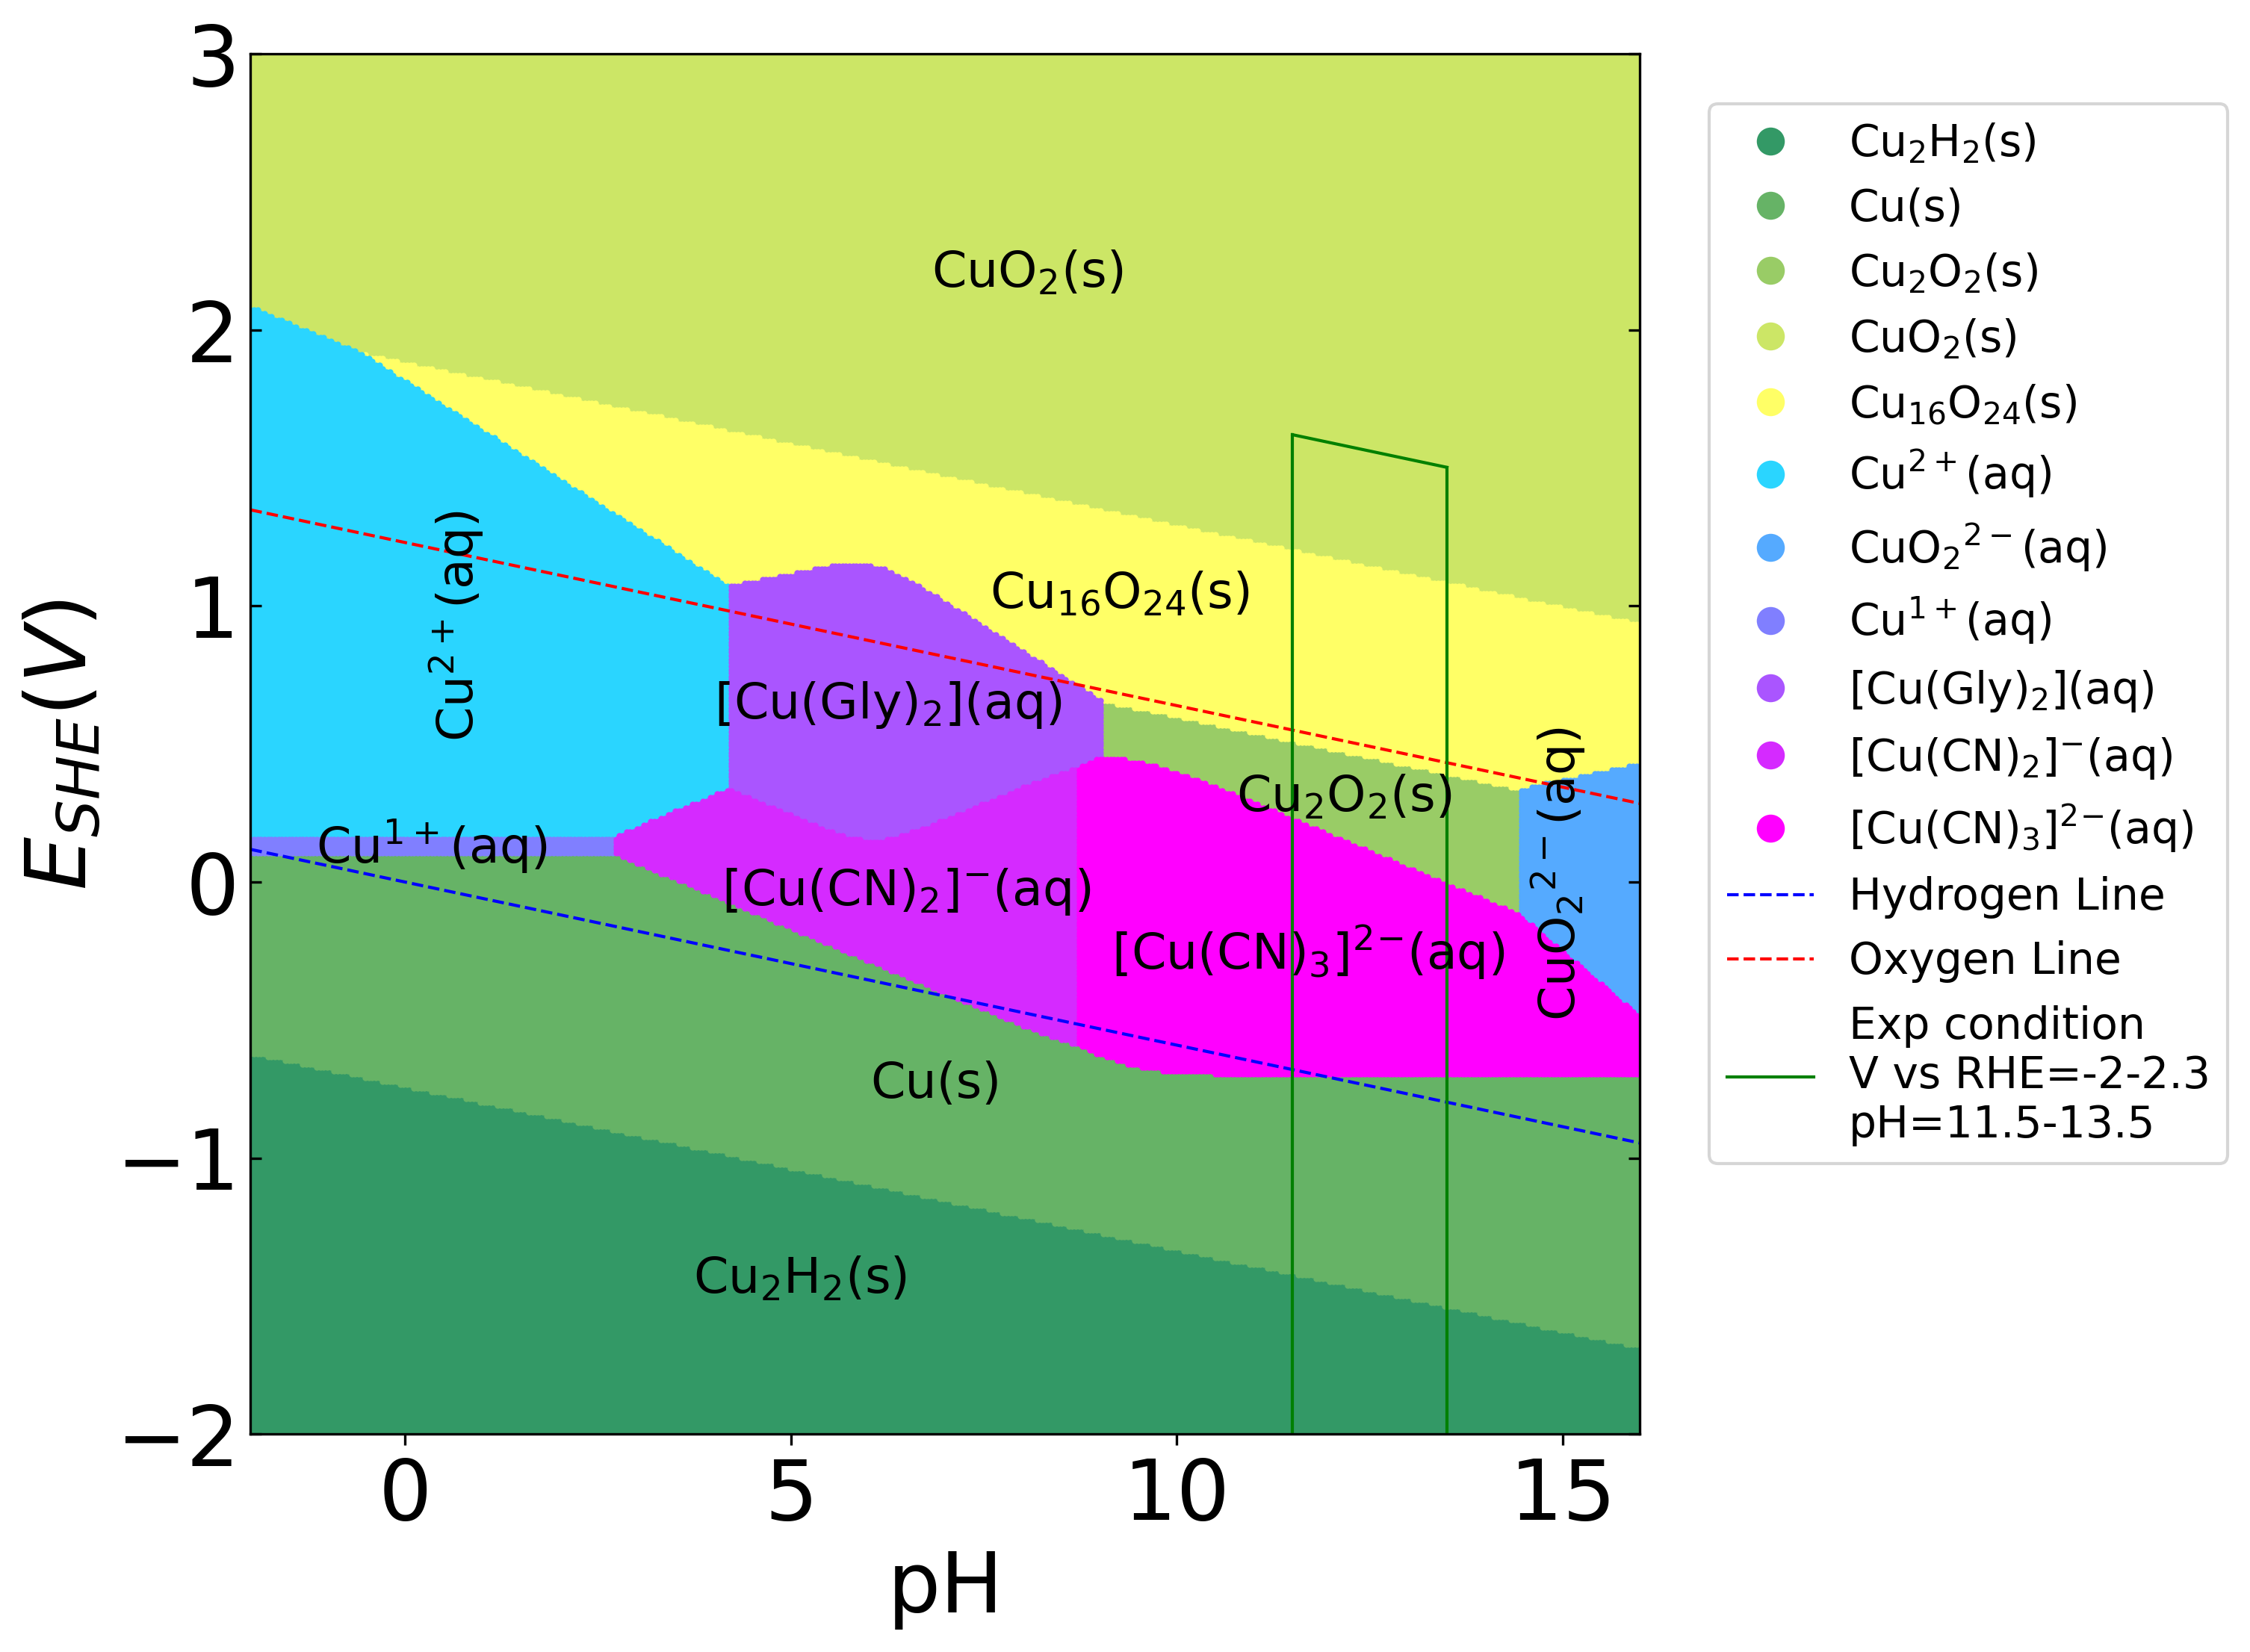
\includegraphics[width=\textwidth]{Figures/pourbaix_diagrams/Cu-NH3-H2O_activity=1e-04_[NH3]=0.02M_[Gly]=0.005M_[CN]=0.0001.png}
%         \par\medskip   
%     \end{subfigure}
%     % Subfigure (d)
%     \begin{subfigure}[b]{0.3\textwidth}
%         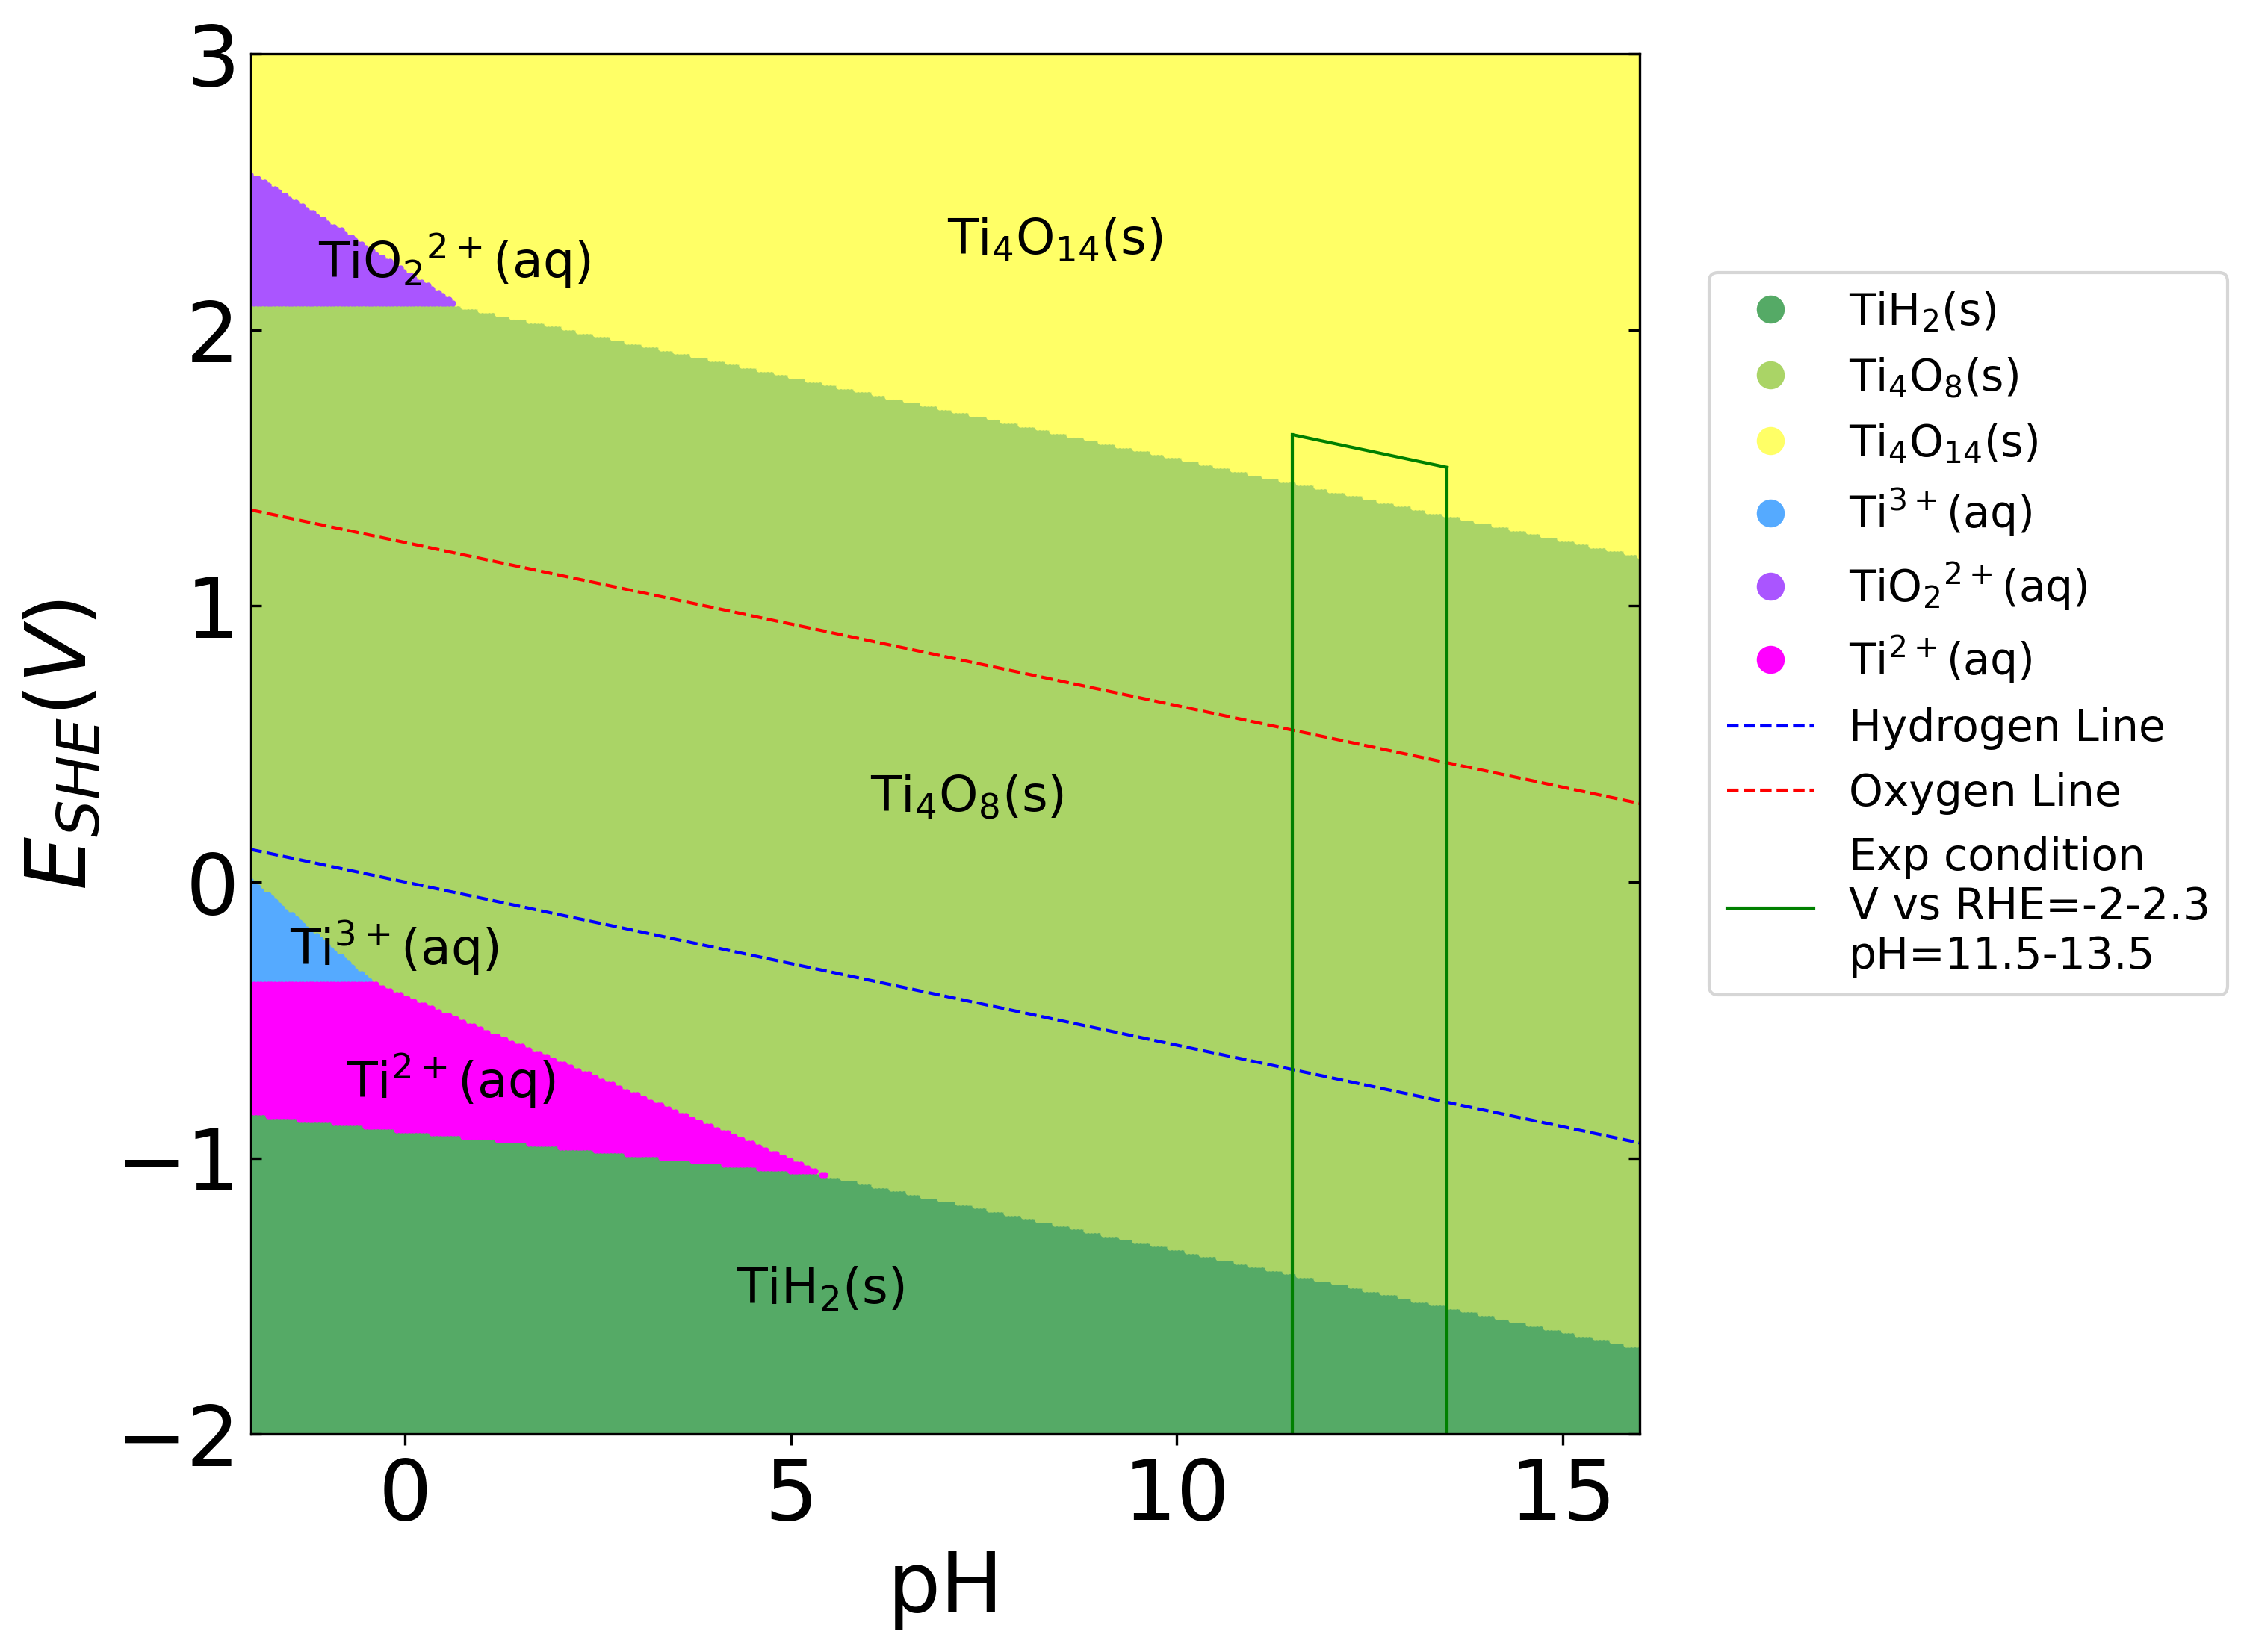
\includegraphics[width=\textwidth]{Figures/pourbaix_diagrams/Ti-NH3-H2O_activity=1e-04_[NH3]=0.02M_[Gly]=0.005M_[CN]=0.0001.png}
%         \subcaption{}\label{fig:Ti_Pourbaix_CN_CH3_Gly}
%     \end{subfigure}
%     % Subfigure (e)
%     \begin{subfigure}[b]{0.3\textwidth}
%         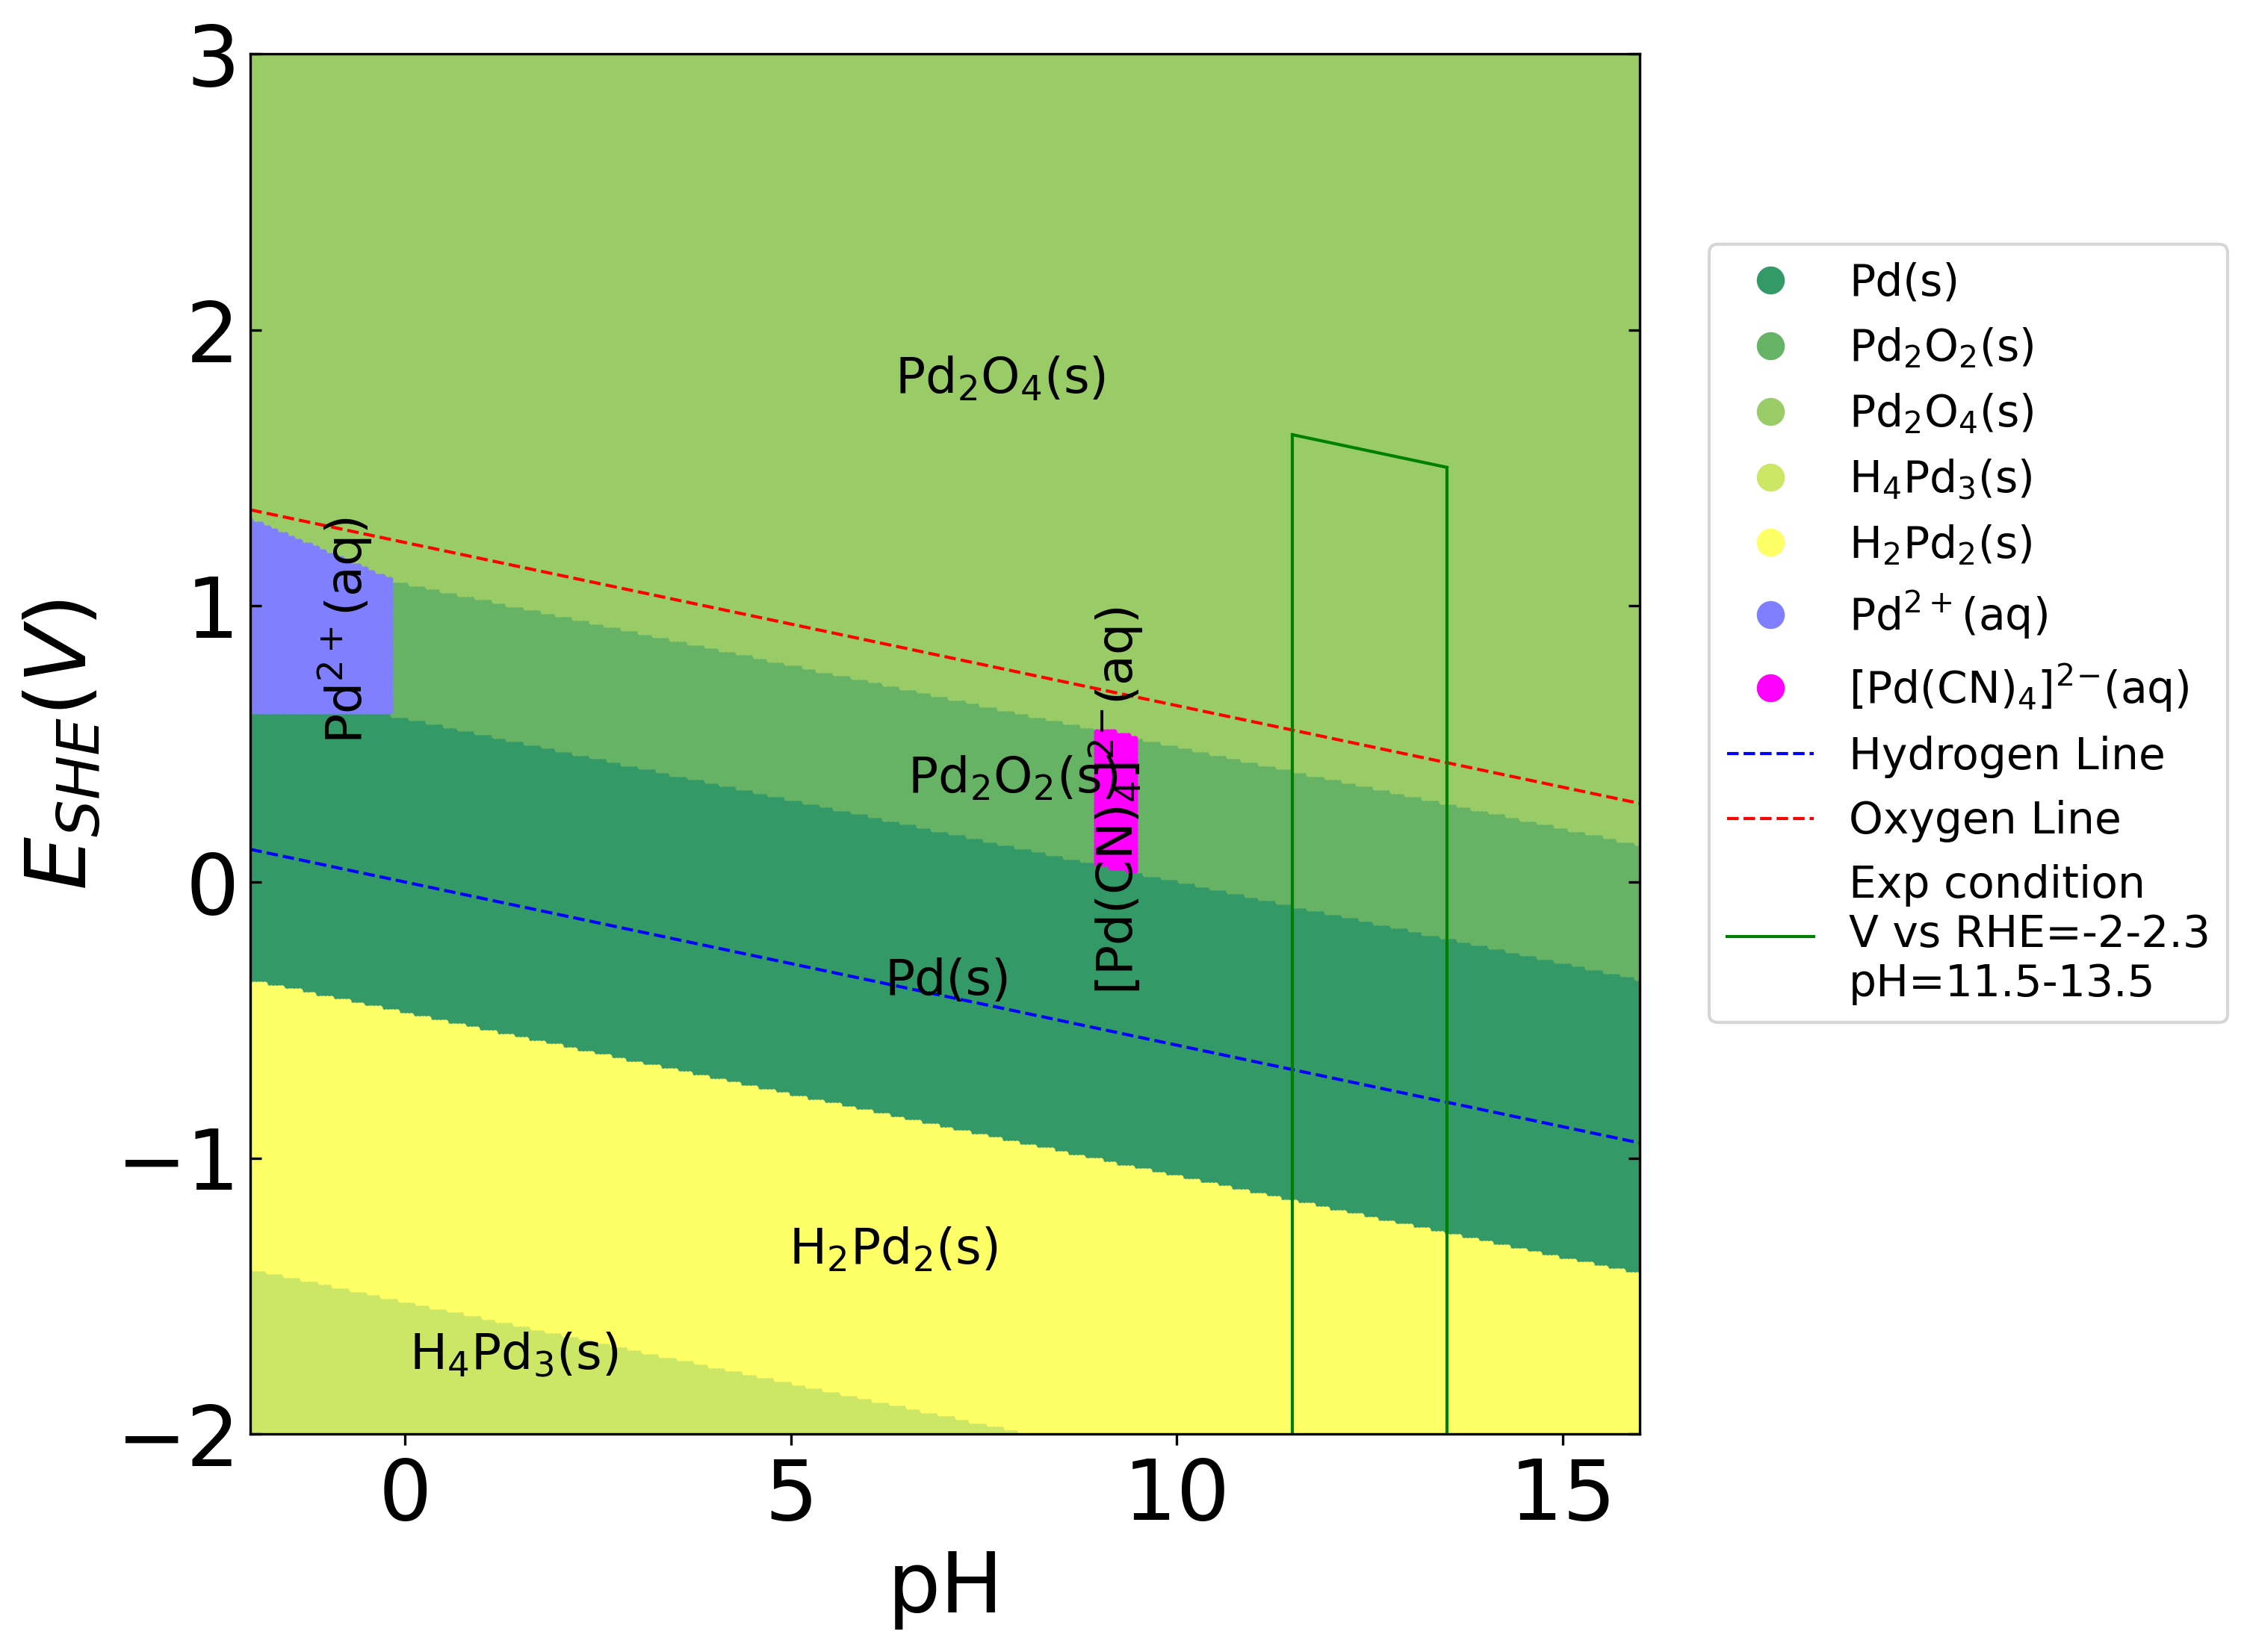
\includegraphics[width=\textwidth]{Figures/pourbaix_diagrams/Pd-NH3-H2O_activity=1e-04_[NH3]=0.02M_[Gly]=0.005M_[CN]=0.0001.png}
%         \subcaption{}\label{fig:Pd_Pourbaix_CN_CH3_Gly}
%     \end{subfigure}
%     % Subfigure (f)
%     \begin{subfigure}[b]{0.3\textwidth}
%         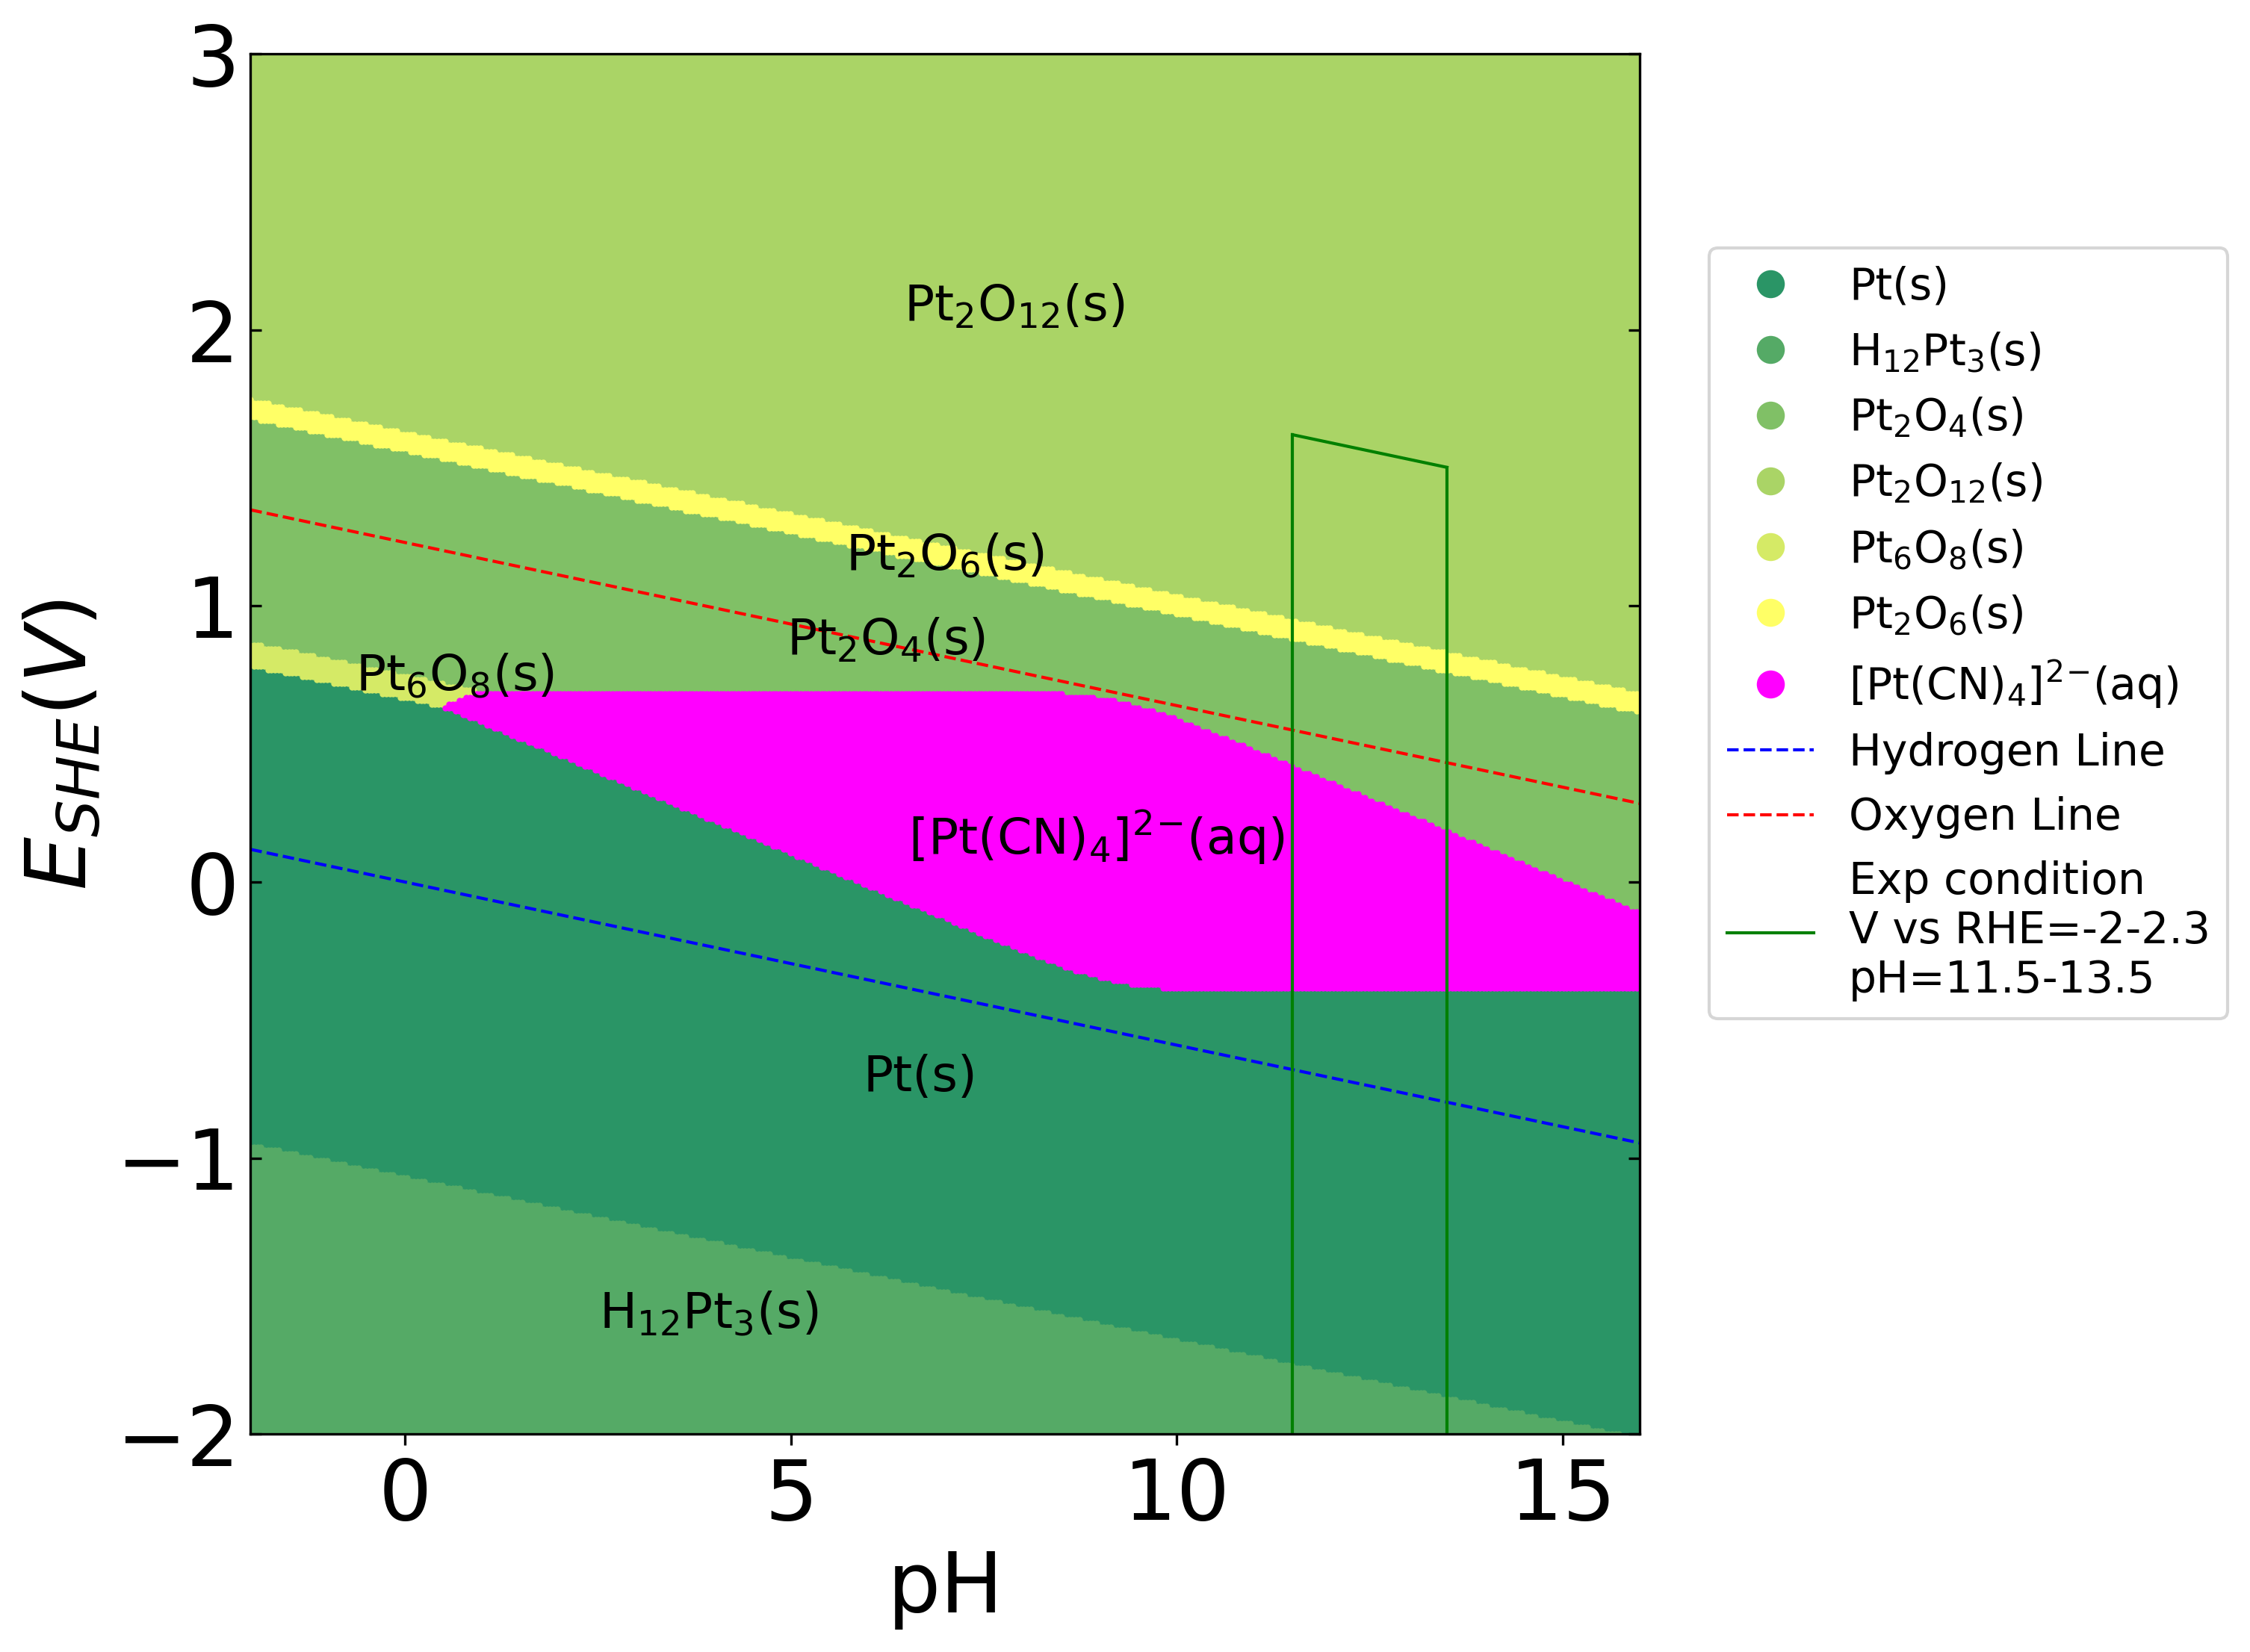
\includegraphics[width=\textwidth]{Figures/pourbaix_diagrams/Pt-NH3-H2O_activity=1e-04_[NH3]=0.02M_[Gly]=0.005M_[CN]=0.0001.png}
%         \subcaption{}\label{fig:Pt_Pourbaix_CN_CH3_Gly}
%     \end{subfigure}

%     \caption{Pourbaix diagrams for metal-\ce{NH3}-\ce{Gly}-\ce{CN-} systems. $[\ce{NH3}]_{initial}= \num{2e-2}M$, $[Gly]_{initial}=\num{5e-3}M$,  $[\ce{CN-}]_{initial}=\num{1e-4}$M. Green box indicates experimental condition at applied potential vs RHE = -2 to 2V, pH = 11.5 to 13.5.}
%     \label{fig:Pourbaix_NH3_Gly}
% \end{figure}



\section{Conclusion}
This study evaluates the stability of Ni, Cu, Pd, Pt, and Ti electrodes under EWAS conditions using Pourbaix diagrams, revealing the significant influence of nitrogen-containing ligands on metal corrosion behavior. While Ni and Cu exhibit strong resistance in aqueous environments, they become highly susceptible to dissolution in the presence of \ce{CN^-} ligands, necessitating careful solution composition control to prevent electrode degradation and contamination. Pd and Pt remain largely unaffected by glycine and ammonia but are vulnerable to cyanide complexation, with uncertainties in reported stability constants further complicating their viability. Given their high cost and instability in cyanide-rich environments, Pd and Pt are not ideal for EWAS applications. In contrast, Ti maintains excellent corrosion resistance due to its passivating oxide layer, making it the most promising candidate despite its low electronic conductivity, which can be addressed through conductive Ti-based materials. These findings highlight the importance of integrating stability considerations into electrode design, ensuring durability and minimizing contamination risks in electrochemical nutrient recovery systems.

